%%%%%%%%%%%%%%%%%%%%%%%%%%%%%%%%%%%%%%%%%%%%%%%%%%%
%% LaTeX book template                           %%
%% Author:  Amber Jain (http://amberj.devio.us/) %%
%% License: ISC license                          %%
%%%%%%%%%%%%%%%%%%%%%%%%%%%%%%%%%%%%%%%%%%%%%%%%%%%

\documentclass[a4paper,11pt, openright]{book}

\raggedbottom %prevents LaTeX from stretching text vertically to fill pages
\widowpenalty=10000
\clubpenalty=10000
\brokenpenalty=10000

\usepackage{csquotes}
\usepackage{amsmath}

\usepackage{tabularx}
\usepackage{array}


\usepackage{longtable}
\usepackage{array}

\usepackage{array}
\usepackage{ltablex}
\keepXColumns

\usepackage{float}   
\usepackage[english]{babel}
\MakeOuterQuote{"}
\usepackage[T1]{fontenc}
\usepackage[utf8]{inputenc}
\usepackage{sectsty}
\usepackage{helvet}
\usepackage{utopia}
\usepackage{setspace}
\usepackage{enumitem} % För att justera avstånd i listor
\usepackage{etoolbox} % För att patcha LaTeX-kommandon
\usepackage{setspace} % För att ställa in radavstånd

\usepackage{array}    % For more flexible column definitions
\usepackage{booktabs} % For better table rules

\allsectionsfont{\sffamily} 

\usepackage{url}
% \usepackage[style=numeric, backend=biber]{biblatex}

\usepackage[style=numeric, backend=biber, sorting=none]{biblatex}


\addbibresource{biblio.bib}
\setcounter{biburllcpenalty}{1}
\setcounter{biburlucpenalty}{0}

\usepackage[a4paper,margin=1.6in,centering]{geometry}
\usepackage{fancyhdr}
\pagestyle{fancy}
\fancyhf{}
\renewcommand{\headrulewidth}{0pt}
\fancyfoot[C]{\thepage} 

\usepackage{tocbibind}
\usepackage{longtable} % For multi-page tables
\usepackage{array}

\usepackage{titlesec}
\titleformat{\chapter}[display]
{\bfseries\fontsize{40}{50}\sffamily}
  {\thechapter} % Label format
  {20 pt} % Space between label and title
  {\Huge} % Before the title


  
% modern I original
%%%%%%%%%%%%%%%%%%%%%%%%%%%%%%%%%%%%%%%%%%%%%%%%%%%%%%%%%
% Source: http://en.wikibooks.org/wiki/LaTeX/Hyperlinks %
%%%%%%%%%%%%%%%%%%%%%%%%%%%%%%%%%%%%%%%%%%%%%%%%%%%%%%%%%
\usepackage{hyperref}
\usepackage{graphicx}
\usepackage{tikz}
\usepackage{tcolorbox}
\usepackage{xcolor}
\definecolor{mylightblue}{RGB}{200,255,255}
%\usepackage[english]{babel}

\newenvironment{myitemize}
  {\begin{itemize}\setstretch{1.15}}
  {\end{itemize}}

\newenvironment{compactitemize}{
  \begin{itemize}[itemsep=0.0em]
}{
  \end{itemize}
}

\linespread{1.15}



%%%%%%%%%%%%%%%%%%%%%%%%%%%%%%%%%%%%%%%%%%%%%%%%%%%%%%%%%%%%%%%%%%%%%%%%%%%%%%%%
% 'dedication' environment: To add a dedication paragraph at the start of book %
% Source: http://www.tug.org/pipermail/texhax/2010-June/015184.html            %
%%%%%%%%%%%%%%%%%%%%%%%%%%%%%%%%%%%%%%%%%%%%%%%%%%%%%%%%%%%%%%%%%%%%%%%%%%%%%%%%
\newenvironment{dedication}
{
   \cleardoublepage
   \thispagestyle{empty}
   \vspace*{\stretch{1}}
   \hfill\begin{minipage}[t]{0.66\textwidth}
   \raggedright
}
{
   \end{minipage}
   \vspace*{\stretch{3}}
   \clearpage
}

%%%%%%%%%%%%%%%%%%%%%%%%%%%%%%%%%%%%%%%%%%%%%%%%
% Chapter quote at the start of chapter        %
% Source: http://tex.stackexchange.com/a/53380 %
%%%%%%%%%%%%%%%%%%%%%%%%%%%%%%%%%%%%%%%%%%%%%%%%
\makeatletter
\renewcommand{\@chapapp}{}% Not necessary...
\newenvironment{chapquote}[2][2em]
  {\setlength{\@tempdima}{#1}%
   \def\chapquote@author{#2}%
   \parshape 1 \@tempdima \dimexpr\textwidth-2\@tempdima\relax%
   \itshape}
  {\par\normalfont\hfill--\ \chapquote@author\hspace*{\@tempdima}\par\bigskip}
\makeatother

%%%%%%%%%%%%%%%%%%%%%%%%%%%%%%%%%%%%%%%%%%%%%%%%%%%
% First page of book which contains 'stuff' like: %
%  - Book title, subtitle                         %
%  - Book author name                             %
%%%%%%%%%%%%%%%%%%%%%%%%%%%%%%%%%%%%%%%%%%%%%%%%%%%


\begin{document}

\frontmatter

% % !TEX root = Thesis.tex
% \pagestyle{empty}


% \begin{Huge}  \sffamily

% \textbf{Design and Implementation of a Web-Based Data Processing and Visualization Prototype for the Volvo CE TMC Workflow}
% \newline
% \end{Huge} 
% \begin{Large} \sffamily
% \bigskip\newline\indent
% % A Case Study of the Volvo CE Total Market Calculation Workflow
% \newline
% \bigskip\bigskip\newline\indent

% \textbf{Yanxiang Du} \newline\newline\indent
% % \textbf{Mary Doe}
% \end{Large}
% \newline\



% \vspace{270pt plus 1pt minus 1pt}
% %\begin{Large} \sffamily
% %\bigskip\newline\indent
% %\textbf{Department of Computer \newline\indent
% %and Systems Sciences}
% %\end{Large}

% %\begin{small} \sffamily
% %\newline\indent
% %\vspace{150pt} \\

% \begin{spacing} {1.55}
    

% \begin{small} \rmfamily
% %\newline\indent
% \begin{minipage}{0.65\textwidth}
% Master's Degree Project in\\\indent
% Master's Programme in Information Security\\\indent
% Spring term 2026\\\indent
% Supervisor: Yuhong Li\\\indent
% Department of Computer \\\indent
% and Systems Sciences
% %Swedish title: XXX
% \end{minipage}
% \end{small}
% \begin{minipage}{0.32\textwidth}
% \begin{center}
%     
\includegraphics[width=0.95
%     \textwidth]{SUloggaeng.png}
% \end{center}
% \end{minipage}
% \end{spacing}

% \newpage
% \thispagestyle{empty}
% \mbox{}


\pagestyle{empty}

\begin{Huge}\sffamily
\textbf{Design and Implementation of a Web-Based Workflow Inspection Prototype for ERP-Based Enterprise Data Processing}
\end{Huge}

\vspace{0.8cm}

\begin{Large}\sffamily
\textbf{A Case Study of Volvo CE's Total Market Calculation Workflow}
\end{Large}

\vspace{2cm}

\begin{Large}\sffamily
\textbf{Yanxiang Du}
\end{Large}

\vfill

\begin{spacing}{1.55}
\begin{minipage}{0.65\textwidth}
\small\rmfamily
Master's Degree Project in\\
Master's Programme in Information Security\\
Spring term 2026\\
Supervisor: Yuhong Li\\
Department of Computer\\
and Systems Sciences
\end{minipage}
\hfill
\begin{minipage}{0.32\textwidth}
\begin{center}

\includegraphics[width=0.95\textwidth]{SUloggaeng.png}
\end{center}
\end{minipage}
\end{spacing}

\newpage
\thispagestyle{empty}
\mbox{}

% !TEX root = Thesis.tex
% \chapter*{Abstract} 
% \addcontentsline{toc}{chapter}{Abstract}
% \pagestyle{plain}

% \paragraph{Introduction} This thesis addresses transparency and usability challenges in Volvo CE's Total Market Calculation (TMC) workflow, which is currently executed in an SAP-based environment. Although the existing process supports required calculations, business users have limited visibility into intermediate transformations, which makes validation and communication with IT more difficult.

% \paragraph{Research Question} The study investigates the following question: \textit{How can an interactive data processing and visualization prototype be designed to improve transparency, traceability, and usability in the Volvo CE TMC workflow?}

% \paragraph{Method} The thesis applies Design Science Research (DSR), following the activities of problem explication, requirement definition, artefact design and development, demonstration, and evaluation. The artefact was implemented as a web-based frontend-backend prototype with Python/FastAPI services, SQL-backed processing, and workflow-oriented visualization for source upload, preparation, adjustment, and split-related stages.

% \paragraph{Results} The prototype was demonstrated with real workflow data from the 2024 calculation cycle. Uploaded source and matrix files were processed successfully, and generated preparation-, adjustment-, and split-related outputs were compared with manually verified reference results. The comparison indicated that the implemented outputs were consistent within the prototype scope. The web interface enabled layer-based inspection, filtering, dynamic summaries, chart-based review, and CSV export.

% \paragraph{Discussion} The artefact shows that selected SAP-embedded workflow logic can be re-expressed in a more transparent and inspectable web-based environment. Main limitations include the prototype scope, controlled evaluation setting, dependency on input data quality, and the need for stronger infrastructure and broader organizational integration for large-scale use.


\chapter*{Abstract}
\addcontentsline{toc}{chapter}{Abstract}
\pagestyle{plain}

\paragraph{Introduction} This thesis addresses transparency, traceability, and usability challenges in ERP-based enterprise data processing implemented in systems such as SAP. Large industrial and manufacturing firms often use such systems for multi-step reporting, planning, and calculation processes, yet business users may have limited visibility into intermediate transformations, which makes validation, error investigation, and communication with IT more difficult. The general problem is investigated through the case of Volvo CE's Total Market Calculation (TMC) workflow.

\paragraph{Research Question} The study investigates the following question: \textit{How can an interactive data processing and visualization prototype be designed and evaluated to enhance transparency, traceability, and usability in ERP-based enterprise data processing?}

\paragraph{Method} The thesis combines Design Science Research (DSR) with a case study. DSR structures the artefact design, development, demonstration, and evaluation, while the Volvo CE case provides the empirical context in which the broader workflow problem is examined. The artefact was implemented as a web-based prototype with a frontend-backend architecture, using React, Python/FastAPI services, SQL-backed processing, and workflow-oriented views for file upload, matrix submission, layer-based inspection, and staged result review.

\paragraph{Results} The prototype was demonstrated using real workflow data from the 2024 TMC calculation cycle at Volvo CE. Uploaded source and matrix files were processed successfully, and the generated preparation, market view, adjustment, machine line split, and resplit outputs were compared with manually verified reference results and selected SAP reference outputs. The comparison indicated that the implemented outputs were largely consistent within the evaluated prototype scope, while observed differences were traced to reference-data version differences or rule-clarification issues.

\paragraph{Discussion} The artefact shows that selected SAP-embedded workflow logic can be re-expressed in a more transparent and inspectable web-based environment. By exposing staged outputs, rule-related fields, and intermediate calculations, the prototype supports business users in reviewing and validating selected workflow stages. The main limitations include the partial workflow scope, the controlled evaluation setting, dependency on input data quality, limited end-to-end row-level lineage, and the need for stronger infrastructure before broader internal use.


\paragraph{Keywords} Total Market Calculation, ERP, ERP-Based Enterprise Data Processing, SAP, Workflow Transparency, Traceability, Construction Equipment Market Analysis\href{}{}









% !TEX root = Thesis.tex
\chapter*{Acknowledgements}
\addcontentsline{toc}{chapter}{Acknowledgements}



I would like to express my sincere gratitude to Volvo Construction Equipment and the Strategy \& Business Development Department for giving me the opportunity to carry out this thesis project in collaboration with them. This experience allowed me to work on a meaningful business problem and to gain valuable insights into how data, market intelligence, and enterprise systems are used in practice.

I am especially grateful to Jacques Mathieu, Madeleine Broberg, and Lian Su for their continuous support throughout the project. I sincerely appreciate the time they spent introducing me to the business background, explaining the Total Market Calculation workflow, and helping me understand the practical challenges behind the existing process. Their patience, constructive discussions, and positive feedback greatly encouraged me during the development of the prototype and helped shape the direction of this thesis.

I would also like to thank my academic supervisor, Yuhong Li, for her guidance and support from an academic perspective. Her feedback helped me improve the structure, methodology, and academic quality of the thesis.

Finally, I would like to thank everyone who has supported and contributed to my thesis work. I am also deeply grateful to my friends in Sweden for their continuous support, companionship, and encouragement throughout this journey.






% !TEX root = Thesis.tex
\chapter*{Abbreviations} 
\addcontentsline{toc}{chapter}{Abbreviations}

\begin{spacing}{1.5}
\begin{longtable}{>{\raggedright\arraybackslash}p{0.25\linewidth}>{\raggedright\arraybackslash}p{0.75\linewidth}}
    \textbf{Abbreviation} & \textbf{Description} \\
    \hline
ABAP & Advanced Business Application Programming \\
API & Application Programming Interface \\
BI & Business Intelligence \\
BW & SAP Business Warehouse \\
CRP & A Volvo CE internal data source that provides industry exchange-related reference data used in the TMC workflow \\
CSV & Comma-Separated Values file format \\
DSR & Design Science Research \\
ERP & Enterprise Resource Planning \\
ETL & Extract, Transform, Load \\
FastAPI & Python web framework used to implement the backend API services \\
FR & Functional Requirement \\
IT & Information Technology \\
OTH & Supplementary external market data \\
PostgreSQL & Relational database management system used for persistent data storage \\
PR & Performance Requirement \\
SAL & Volvo CE internal sales data \\
SAP & Enterprise software platform and environment developed by SAP SE \\
SQL & Structured Query Language \\
TMA & Total Market reference data used in the TMC workflow \\
TMC & Total Market Calculation \\
UI & User Interface \\
Volvo CE & Volvo Construction Equipment \\
VCE & Volvo Construction Equipment \\
\end{longtable}
\end{spacing}


\listoffigures
\listoftables
\tableofcontents

\mainmatter

% !TEX root = ../Thesis.tex
\chapter{Introduction} \label{cha:introduction}
\pagestyle{plain}






% Transparency and traceability have become critical concerns in data-driven decision-making environments as the complexity of enterprise data ecosystems continues to increase.\cite{kernstock2025dataecosystems} In industries such as construction equipment, organizations rely on integrating heterogeneous data sources, including internal sales data and external market intelligence, to support market analysis and strategic decision-making.\cite{moller2024industrial} Due to differences in data formats, classification standards, and regional business rules, companies must design complex data processing approaches to harmonize and reconcile these datasets in order to approximate real market conditions.\cite{cheng2024harmonization} 

% To support business operations such as market share analysis, these data are typically processed through complex calculation frameworks implemented in enterprise systems such as SAP.\cite{gessa2023erp} While enterprise systems such as SAP provide strong capabilities for large-scale data processing, their operation is not always fully transparent to end users, particularly when data transformations depend on system configurations, integration mechanisms, and business rules that are not directly visible in everyday use.\cite{acev2025datagovernance} This lack of transparency and traceability makes it difficult to understand how outputs are generated, validate the correctness of results, and identify potential inconsistencies in the data processing pipeline.\cite{foidl2024pipeline} In addition, the separation between business users and technical system implementations introduces communication barriers, making it challenging to adapt or refine business rules efficiently.\cite{ori2024misalignment}


% Building on these challenges, Volvo Construction Equipment (Volvo CE) encounters similar issues in the calculation of market share, where complex business logic is applied to integrate multiple data sources and produce aggregated results. The calculation process relies on SAP-based systems to execute a series of transformations, mappings, and adjustments. However, due to the complexity of the calculation logic and the lack of transparency in the system, business users are unable to trace how input data is transformed into final outputs, nor can they easily verify whether the implemented logic aligns with business requirements. This results in reduced trust in the system, increased difficulty in debugging, and inefficiencies in collaboration between business and IT stakeholders.

% To address these challenges, this thesis adopts a Design Science Research approach and proposes the design and implementation of a data processing and visualization system. The proposed solution aims to improve transparency and traceability by reconstructing the calculation logic as a structured data pipeline, enabling users to trace data transformations, validate results, and interact with the system more effectively. By bridging the gap between business understanding and technical implementation, the system supports more efficient error detection, rule adjustment, and data-driven decision-making. 

% \ref{fig:pipe}.

% \begin{figure} [h]
% \centering
% 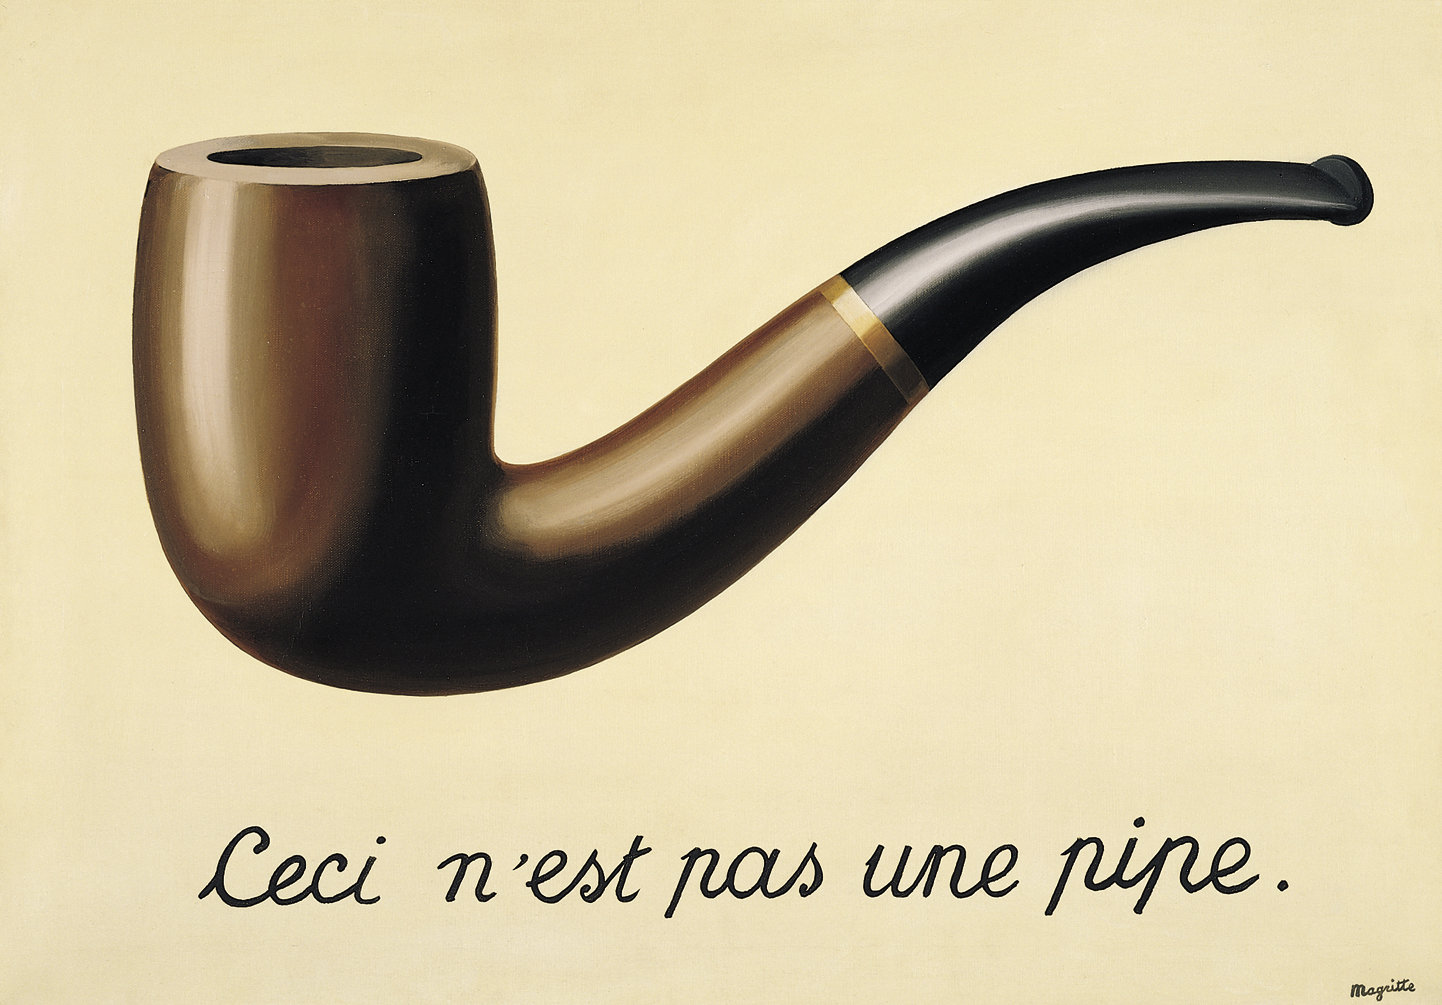
\includegraphics[scale = 0.8]{pipe.jpg}
% \caption{A Picture of a Pipe}
%  \label{fig:pipe}
% \end{figure}
% \section{Overall Background}

% Volvo Construction Equipment (Volvo CE) is a subsidiary of the Volvo Group and operates as a global provider of construction solutions, with its products and services available in more than 140 countries. This thesis is conducted within the Global Business Intelligence department, where market-related data is processed and analyzed to support business understanding across countries, regions, and product categories.

% The construction equipment industry is characterized by considerable complexity. Variations in machine lines, size classes, and regional market conditions make it difficult to establish a consistent view of the market. Market-related data is further drawn from multiple internal and external sources that frequently differ in structure, naming conventions, and classification rules. Structured processing is therefore required to reconcile heterogeneous datasets and establish a consistent foundation for reporting and market share analysis.

% Within Volvo CE, this need is addressed through Total Market Calculation (TMC), an internal process designed to prepare market data for reporting and market share analysis. TMC operates within an SAP BW-based environment, encompassing objects such as ADSOs, cubes, process chains, and planning sequences, alongside matrices that govern how sources, countries, brands, machine lines, and size classes are interpreted during processing. Certain parts of the workflow are additionally managed through portal pages and Analysis for Office workbooks.

% The workflow begins with data input. TMC integrates data from two primary sources: the internal Corporate Reporting Platform data (CRP) system and other external market files (OTH). CRP provides the principal market inputs, including total market data (TMA), detailed market data, and Volvo CE internal sales-related data (SAL). Since the total market in CRP is derived from brands participating in the statistical exchange, and not all brands contribute to it, external sources are incorporated to supplement this market view.

% The subsequent stage concerns data preparation. Prior to calculation, uploaded data must be cleaned and aligned — particularly for external files, which may contain inconsistent brand names, machine line designations, or size-class structures. To support this process, TMC employs a set of mapping and rule tables, including the Reporter List, Source Matrix, Country Group Matrix, and size-class-related tables, which govern source selection, brand treatment, and size-class handling in subsequent steps.

% Following the preparation of the data foundation, TMC proceeds through a series of calculation stages: preparation, adjustment, split, total market calculation, and restatement. The preparation stage establishes the initial calculation basis, while adjustment aligns values with the total market logic. The split stage redistributes data across machine lines and size classes where source data is not available at the required level of granularity. Total market calculation then consolidates market values, and restatement recalculates final values for reporting purposes. These stages are executed sequentially, as each subsequent step is dependent on the output of its predecessor.

% The present thesis focuses on the segment of the TMC workflow spanning from data input through the preparation and adjustment stages — the phase in which data from internal and external sources is uploaded, cleaned, aligned, and converted into the foundation for subsequent calculation steps.

% Although this SAP-based setup provides a formal and operational way to run market-related calculations, the underlying logic is difficult for business users to follow. Business users may see the final results in reports, but they cannot easily trace how a value has been derived across different SAP objects, mappings, and calculation steps. As a result, the process becomes difficult to validate from a business perspective, and communication between business stakeholders and technical teams becomes more challenging when rules need to be checked or adjusted. It is within this context that the present thesis is positioned.



% \subsection{A Subsection}
% Here is the first subsection of the first section.


\section{Background}
\pagestyle{plain}
As enterprise data ecosystems grow in complexity, organizations increasingly rely on workflows that integrate heterogeneous data sources, apply rule-based transformations, and generate analytical outputs for decision-making \cite{putrama2024heterogeneous,cheng2024harmonization}. In such settings, enterprise platforms such as SAP provide strong capabilities for data integration, processing, and reporting \cite{gessa2023erp,sap_erp_guide}. However, when transformations depend on embedded configurations, mappings, and system-specific execution logic, it becomes difficult for business users to understand how outputs are generated, validate intermediate results, and identify where inconsistencies arise \cite{acev2025datagovernance,foidl2024pipeline,ori2024misalignment}.

This challenge is not unique to one organization. It is characteristic of enterprise data-processing workflows in which multiple inputs, rule structures, and staged transformations must be coordinated to produce reviewable outputs. The construction equipment industry provides a suitable case context because market analysis depends on combining internal sales data, external market inputs, and business-specific classification rules across countries, product categories, and machine segments \cite{cece2025,mordor2024construction,moller2024industrial}.

In this thesis, the problem is investigated through the case of Volvo Construction Equipment (Volvo CE), where market share estimation is supported by an SAP-based Total Market Calculation (TMC) workflow. In the studied setting, business users have limited visibility into how uploaded data, mappings, and calculation rules contribute to intermediate and final outputs. This creates difficulties for validation, error investigation, and communication between business and IT stakeholders.

To address this type of problem, the thesis adopts a Design Science Research approach and designs a web-based data processing and visualization prototype that re-expresses selected workflow logic in a more inspectable form. The Volvo CE case serves as the empirical setting in which this broader problem of transparency, traceability, and usability in enterprise data-processing workflows is examined.





\section{Problem and Motivation}
The studied TMC workflow is executed within an SAP BW-based environment where data loading, mapping, transformation, and reporting are distributed across multiple technical objects \cite{wong2016sap}. Although this setup supports the required calculations, it offers limited visibility into intermediate logic from a business-user perspective. As a result, discrepancies are difficult to investigate, rule behaviour is hard to inspect directly, and communication between business and IT becomes more effortful.

These problems are practically significant in the Volvo CE case, but they also reflect a broader design problem: enterprise data-processing workflows often prioritize execution correctness over inspectability for non-technical users. The motivation for this thesis therefore lies not only in improving one specific workflow, but in exploring how such workflows can be re-expressed in a form that better supports transparency, traceability, and validation. The Volvo CE setting provides a concrete case through which this more general problem can be investigated.










% \section{Research Goal}
% The goal of this thesis is to design and implement an interactive data processing and visualization prototype for the Volvo CE TMC workflow, focusing on improving transparency, usability, and traceability in the preparation and adjustment stages of the calculation process.

% The current TMC process relies on a complex SAP-driven workflow integrating multiple data sources — TMA, SAL, CRP, OTH, and matrix-based business rules — whose logic is difficult to trace and interpret from a user perspective. This thesis explores how a modern web-based prototype can make this workflow more visible and accessible by presenting key data inputs, intermediate layers, and adjustment results in a clearer, more interactive way, translating essential business logic into a system that supports data upload, rule handling, table exploration, and result visualization.

% The main research question is:
% How can an interactive data processing and visualization prototype be designed to improve transparency, traceability, and usability in the Volvo CE TMC workflow?
% This is addressed through three sub-questions:

% \textbf{Sub-RQ1:} How can a web-based system support the upload, management, and display of workflow input files so that different source datasets and matrix-based business input become easier to access and inspect? \\

% \textbf{Sub-RQ2:} How can the workflow stages of preparation, adjustment, and split be represented in a web-based system so that users can more clearly follow how results are derived from CRP, SAL, OTH, and related business rules? \\

% \textbf{Sub-RQ3:} How can interactive UI elements, such as filtering, summary calculations, chart-based displays, and layer-based views, improve usability and support validation of intermediate and derived workflow results? \\



% The expected outcome is a deployable web-based prototype system that re-expresses selected parts of the TMC workflow in a more accessible and inspectable environment, while also providing a foundation for future broader internal deployment and extension to later workflow stages.



\section{Research Objective and Research Question}

The current TMC process integrates multiple data sources — TMA (Total Market reference data), SAL (Volvo CE internal sales data), OTH (supplementary external market data), and matrix-based business rules — within an SAP-driven environment whose logic is difficult to trace and interpret from a business user perspective.

The goal of this thesis is to design and implement an interactive data processing and visualization prototype for the Volvo CE TMC workflow that improves transparency, usability, and traceability in the preparation stage, including market-view derivation, as well as the adjustment and machine line split stages, by translating the underlying business logic into a web-based system that supports data upload, staged processing, and interactive result inspection.


The main research question is:
How can an interactive data processing and visualization prototype be designed and evaluated to enhance transparency, traceability, and usability in complex enterprise data-processing workflows?
This is addressed through three sub-questions:

\textbf{Sub-RQ1:} How can the architecture and data handling of a web-based prototype be designed to support structured upload, storage, and management of heterogeneous workflow inputs, including source datasets and matrix-based business rules?\\

\textbf{Sub-RQ2:} How can staged data-processing activities be re-expressed in a web-based environment so that intermediate transformations and derived results become inspectable and traceable for business users?\\

\textbf{Sub-RQ3:} To what extent does the implemented prototype improve transparency, usability, and traceability compared to an existing SAP-based workflow representation, as assessed through demonstration and stakeholder feedback?\\

The expected outcome is a working web-based prototype that demonstrates how selected enterprise workflow logic can be re-expressed in a more accessible and inspectable environment, while still being grounded in a realistic industrial case.









% \section{Scope and Delimitation}
% This thesis focuses on the design and implementation of a web-based prototype for the Volvo CE TMC workflow, based on the existing SAP-driven calculation process that integrates multiple data sources, business rules, and matrix-based mappings.

% The scope is limited to the preparation and adjustment stages, which cover source data integration, rule-based mapping, intermediate data transformation, and adjustment logic. The prototype is designed to make these stages more transparent, interactive, and easier to understand through a modern frontend-backend system. It includes interfaces for data upload, workflow navigation, layer-based visualization, and interactive table exploration, as well as filtering, summary calculations, and clearer presentation of intermediate results.

% The thesis does not aim to replace the existing SAP system or implement the full TMC workflow. Later stages — such as split, total market restatement, and full rule automation — are treated as future development rather than part of the current scope.

% The authentication and account management functions are implemented as a local development solution only, and are not intended as a production-ready architecture. Any real deployment would require alignment with Volvo CE's internal IT infrastructure and security requirements.

% This thesis should therefore be understood as an initial but functional prototype that demonstrates how the preparation and adjustment logic of the TMC workflow can be translated into a more transparent, extensible, and user-friendly system.



% \section{Scope and Delimitation}

% This thesis focuses on the design and implementation of a web-based prototype for the Volvo CE TMC workflow, based on the existing SAP-driven calculation process that integrates multiple data sources, business rules, and matrix-based mappings.

% The scope covers the preparation, adjustment, and selected split-related stages of the workflow. These stages include source data integration, rule-based mapping, intermediate data transformation, adjustment logic, and inspectable split and re-split behaviour for selected cases. The prototype is designed to make these stages more transparent, interactive, and easier to understand through a modern frontend-backend system. It includes interfaces for data upload, workflow navigation, layer-based visualization, and interactive table exploration, as well as filtering, summary calculations, and clearer presentation of intermediate and derived results.

% The thesis does not aim to replace the existing SAP system or implement the full TMC workflow. Later stages, such as total market calculation, restatement, and reporting, are treated as future development rather than part of the current scope.

% % The authentication and account management functions are implemented as a local development solution only, and are not intended as a production-ready architecture. Any real deployment would require alignment with Volvo CE's internal IT infrastructure and security requirements.

% This thesis should therefore be understood as an initial but functional prototype that demonstrates how selected TMC workflow logic, including preparation, adjustment, and Machine line split-related processing, can be translated into a more transparent, extensible, and user-friendly system.

\section{Scope and Delimitation}

This thesis focuses on the design and implementation of a web-based prototype for selected stages of the Volvo CE TMC workflow. The implemented scope covers source-data upload, matrix input handling, preparation, market-view derivation, adjustment, and selected split/resplit-related processing. The prototype provides interfaces for workflow navigation, layer-based visualization, interactive table exploration, filtering, summary calculation, and CSV export.

The thesis does not aim to replace the existing SAP system or implement the full TMC workflow. Full Total Market Calculation, full Restatement, and final Reporting remain outside the implemented scope. The case setting is used to study a broader workflow-design problem, but the empirical evaluation is still bounded to the selected TMC stages and the available organisational context.








\section{Thesis Structure}

Following this introduction, the thesis is structured into six further chapters. The background chapter introduces enterprise workflow transparency issues and the Volvo CE case context. The methodology chapter describes the Design Science Research approach used in the study. The problem and requirements chapter defines the design problem and presents the requirements for the prototype. The artefact chapter explains the design and implementation of the web-based prototype. The evaluation chapter presents the demonstration and assessment of the prototype using the case setting. Finally, the discussion chapter answers the research questions, discusses contributions and limitations, and suggests future work.


% !TEX root = ../Thesis.tex




\chapter{Extended Background} \label{cha:extendBackground}



This chapter provides the background for the thesis. It first introduces ERP systems and SAP as a general enterprise data-processing environment, then presents the industry and Volvo CE case context, outlines broader challenges in SAP-based enterprise workflow implementations, and finally reviews related work relevant to transparency, traceability, and usability in enterprise analytics.


\section{ERP Systems, SAP, and Enterprise Workflows}

Enterprise resource planning (ERP) systems are widely used to integrate and manage core business processes across large organizations \cite{davenport1998,klaus2000}. Rather than treating finance, operations, procurement, manufacturing, logistics, and sales as isolated activities, ERP systems provide a shared environment in which data and processes can be coordinated across functional boundaries \cite{sap_erp_guide}. In that sense, ERP should be understood not only as a transactional business system, but also as an enterprise data-processing setting environment in which important reporting, planning, and calculation processes are executed.

Prior literature indicates that ERP-based environments can support activities beyond basic transaction processing. Integrated enterprise data may also be reused for reporting, planning, performance monitoring, and analytical routines in different organizational settings \cite{monk2012erp,fan2006equipmentdw}. In this thesis, this is taken as support for viewing complex business calculations in enterprise systems as part of a broader workflow context rather than only as an isolated practice in one company.

SAP is one of the most widely used ERP platforms in this broader landscape. Within SAP-based environments, workflow execution is often distributed across data-loading mechanisms, storage structures, transformation logic, reporting layers, and user-facing interfaces. This makes SAP relevant to the present thesis not because it is unique to Volvo CE, but because it represents a common type of enterprise environment in which complex data-processing workflows are embedded.

Within the SAP landscape, transactional processing and analytical processing are typically separated. Operational data is generated in ERP systems, while SAP Business Warehouse (BW) provides an analytical layer for reporting, modeling, and transformation \cite{sap_bw_guide}. SAP also supports structured data loading, multidimensional storage, sequential rule execution, and spreadsheet-based user interaction \cite{sap_bw_ip_overview,sap_analysis_office_guide}. These capabilities make SAP suitable for complex multi-step workflows, but they also contribute to technical complexity.

This complexity is also reflected in prior work. Research on SAP ERP process extraction describes the identification of relevant process structures and related tables as a significant challenge because SAP ERP contains a large amount of process and data complexity \cite{weber2022sap}. ERP usability studies further report difficulties related to navigation, task support, learnability, and presentation of outputs \cite{calisir2004erp,wong2016sap}. Together, these studies support treating transparency, traceability, and usability as relevant concerns in ERP-based enterprise data processing beyond one company-specific case.




\section{Construction Equipment Industry and Market Share Estimation}




% The construction equipment industry is a global, capital-intensive sector supporting infrastructure development, mining, and urbanization. Leading manufacturers include Volvo Construction Equipment (Volvo CE), Caterpillar, Komatsu, Hitachi Construction Machinery, and Liebherr, all operating across multiple regions with diverse product portfolios \cite{offhighway2024report,statista2024construction}. These manufacturers maintain global distribution networks and sell equipment across a large number of countries, reflecting the highly international nature of the industry \cite{volvo2024annual}.

% Construction equipment is typically organized into machine lines, which represent major categories of machinery based on functionality. Common machine lines include hydraulic excavators, wheel loaders, articulated haulers, rigid haulers, and road construction equipment. Within each machine line, products are further segmented into size classes, usually defined by operating weight ranges (e.g., <6 tons, 6–10 tons, >10 tons), reflecting different application scenarios and customer needs \cite{mordor2024construction}.

% From a market analysis perspective, the industry is structured along dimensions including country, machine line, size class, and brand. Market size and share are therefore calculated at a granular level, allowing companies to evaluate performance in specific segments.

% To support market analysis, companies integrate multiple data sources. Internal data consists of sales records from enterprise systems.Companies also participate in industry data exchange systems, where aggregated sales information is shared among manufacturers to estimate total market size, often coordinated by industry associations or specialized providers such as Off-Highway Research \cite{offhighway2024report,offhighway2018method}. External datasets from third-party providers, dealer networks, and national registration systems further complement these sources, improving market coverage where direct reporting is limited \cite{mordor2024construction,oxford2023equipment}. These datasets are standardized and integrated to ensure consistency across countries, machine lines, and brands.
This thesis is grounded in the case of Volvo Construction Equipment (Volvo CE), whose market-analysis work is situated in the construction equipment industry. Industry reports describe a market that spans multiple countries, product segments, and regional conditions \cite{cece2025,mordor2024construction}. Because manufacturers operate across these dimensions, market analysis often depends on combining inputs for total market size and market share across regions and product categories.





% Market share is a widely used indicator to evaluate a firm’s competitive position within a defined market. It is typically defined as the ratio between a company’s sales and the total market size within a given segment \cite{kotler2016marketing}. In practice, business units within companies estimate both the total market size and their own share in order to assess competitive dynamics, benchmark performance against competitors, and support strategic planning and decision-making \cite{porter2008competitive}.

% In the construction equipment industry, estimating total market size requires integrating information from multiple sources. A common approach is based on the aggregation of sales data from different manufacturers. Industry intelligence providers such as Off-Highway Research collect and consolidate equipment sales data across regions and product categories, using inputs from manufacturers, dealers, and regional experts to construct a comprehensive view of the market \cite{offhighway2024report,offhighway2018method}. In practice, some manufacturers contribute aggregated sales data to industry research providers or participate in data exchange mechanisms, enabling the construction of comprehensive market statistics \cite{offhighway2018method,mordor2024construction}.

% In addition to manufacturer-reported data, external datasets are often used to complement market coverage. These may include dealer-reported sales, equipment registration statistics, and country-level estimates obtained from third-party providers. Such data sources are particularly important in markets where direct reporting is incomplete or inconsistent.Furthermore, some market research approaches incorporate statistical estimation and modelling techniques. These methods combine historical data with primary and secondary research, and in some cases use macroeconomic indicators to support market estimation and forecasting \cite{mordor2024construction,oxford2023equipment}.

% Based on these practices, data used for market share estimation in the construction equipment industry can generally be categorized into three types: internal company data, industry-level exchange or aggregated data, and external datasets obtained from third-party sources. These different data sources are typically combined to construct a consistent representation of the total market across countries, equipment types, and brands.



% % \section{Market Share Calculation in SAP Systems}


% % At Volvo CE, market share estimation is implemented through a structured Total Market Calculation (TMC) framework that integrates multiple datasets to reconstruct the total market and derive Volvo CE's competitive position.
% % The framework is built on three main data categories: internal sales data (SAL), representing Volvo CE's actual sales volumes; statistical exchange data (CRP) aggregated into total market data (TMA), providing a baseline estimate of overall market size; and additional external datasets (OTH), such as PIN and DES files, extending market coverage. Since these sources differ in structure, they are first transformed into standardized templates before further processing.

% % To enable consistent transformation, the framework relies on predefined matrices and configuration tables, including the Source Matrix, Reporter List, Country Grouping, Brand Mapping, and Size Class structures, which define how data is classified, aggregated, and linked across dimensions.
% % The total market is constructed using a hybrid logic: statistical exchange data provides the initial market size estimate, but since not all brands participate in reporting, the framework incorporates Volvo CE's internal sales data and applies transformation rules to reconstruct a more complete market representation. The implementation of this framework can be understood as a sequence of structured transformation steps, as summarized in Table 2.1.

% % \begin{table}[h]
% % \centering
% % \caption{Step-wise Process of the Market Share Framework at Volvo CE}
% % \label{tab:tmc_process}
% % \begin{tabular}{cll}
% % \toprule
% % \textbf{Step} & \textbf{Phase} & \textbf{Description} \\
% % \midrule
% % 1 & Data Collection & Regional data is collected from CRP, OTH files, and internal sales systems \\
% % 2 & Data Standardization & Input datasets are transformed into standardized templates \\
% % 3 & Matrix Application & Configuration tables (Source Matrix, Reporter List, Brand Mapping) are applied \\
% % 4 & Total Market Construction & Total market (TMA) is constructed based on statistical exchange data \\
% % 5 & Internal Data Integration & Volvo CE sales data (SAL) is integrated into the dataset \\
% % 6 & Reporter Identification & Brands are classified as reporting or non-reporting \\
% % 7 & Estimation of Missing Data & Volumes for non-reporting brands are estimated using rules \\
% % 8 & Segmentation and Allocation & Data is distributed across country, machine line, and size class \\
% % 9 & Market Share Calculation & Market share is calculated as Volvo sales divided by total market \\
% % \bottomrule
% % \end{tabular}
% % \end{table}



% % A defining characteristic of the framework is its multi-dimensional structure, where market share is calculated across country, machine line, and size class. For non-reporting brands where detailed breakdowns are unavailable, volumes are distributed across size classes based on the observed structure of the total market.

% % Overall, the TMC framework can be understood as a rule-based data integration and transformation system that combines internal and external sources to approximate market conditions through predefined matrices and sequential calculation steps.




% Market share is a widely used indicator to evaluate a firm’s competitive position within a defined market. It is typically defined as the ratio between a company’s sales and the total market size within a given segment \cite{kotler2016marketing}. In practice, business units within companies estimate both the total market size and their own share in order to assess competitive dynamics, benchmark performance against competitors, and support strategic planning and decision-making \cite{porter2008competitive}.




% Given the global and highly competitive nature of the construction equipment industry, manufacturers must continuously assess their performance across regions, product segments, and competitors. In this context, understanding market share becomes essential, as it provides a standardized indicator for evaluating competitive position, benchmarking against competitors, and supporting strategic planning and decision-making \cite{porter2008competitive, kotler2016marketing}. 



% However, due to the fragmented nature of data sources and the lack of a unified reporting standard across the industry, there is no universally accepted methodology for calculating total market size and market share. As a result, companies must estimate the total market and their relative position by integrating multiple data sources and applying internal assumptions and transformation rules. Consequently, companies require reliable and structured methods to estimate both the total market size and their market share, which motivates the need for systematic market share estimation approaches discussed in the following section. 












% In the construction equipment industry, estimating total market size requires integrating information from multiple sources. A common approach is based on the aggregation of sales data from different manufacturers. Industry intelligence providers such as Off-Highway Research collect and consolidate equipment sales data across regions and product categories, using inputs from manufacturers, dealers, and regional experts to construct a comprehensive view of the market \cite{offhighway2024report, offhighway2018method}. In practice, some manufacturers contribute aggregated sales data to industry research providers or participate in data exchange mechanisms, enabling the construction of comprehensive market statistics \cite{offhighway2018method, mordor2024construction}.

% In addition to manufacturer-reported data, external datasets are often used to complement market coverage. These may include dealer-reported sales, equipment registration statistics, and country-level estimates obtained from third-party providers. Such data sources are particularly important in markets where direct reporting is incomplete or inconsistent.\cite{mordor2024construction, oxford2023equipment}.

% Based on these practices, data used for market share estimation in the construction equipment industry can generally be categorized into three types: internal company data, industry-level exchange or aggregated data, and external datasets obtained from third-party sources. These different data sources are typically combined to construct a consistent representation of the total market across countries, equipment types, and brands. However, the integration of such heterogeneous data sources also introduces several challenges for enterprise-level implementation.

% First, structural and semantic inconsistencies arise because different data sources often follow different classification standards, levels of granularity, and reporting logic. For example, equipment categories, size classes, and brand definitions may not be aligned across sources, requiring complex mapping and transformation rules to ensure comparability.

% Second, data completeness is often limited. Not all manufacturers participate in data exchange mechanisms, and external datasets may only provide partial market coverage in certain regions. As a result, companies must reconstruct the total market using a combination of reported data and estimation logic, which increases the complexity of the calculation process.

% Third, maintaining consistency across multiple analytical dimensions, such as country, machine line, brand, and time, is challenging when combining heterogeneous datasets. Ensuring that aggregated values remain coherent across different levels of analysis requires carefully designed data processing logic.

% Finally, when such calculation processes are implemented within enterprise systems, additional challenges related to transparency and traceability arise. The underlying calculation logic is often embedded within complex system workflows, making it difficult for business users to understand, validate, or debug intermediate results.

% These challenges highlight the need for structured data processing frameworks that can integrate heterogeneous data sources while ensuring consistency, transparency, and maintainability in market share estimation.


% \subsection{Market Share Estimation in the Construction Equipment Industry and Associated Challenges}

% Given the global and highly competitive nature of the construction equipment industry, manufacturers must continuously assess their performance across regions, product segments, and competitors. In this context, market share serves as an important indicator for evaluating competitive position, benchmarking performance, and supporting strategic planning and decision-making \cite{porter2008competitive, kotler2016marketing}. However, due to the fragmented nature of available data and the lack of a unified reporting standard across the industry, there is no universally standardized methodology for calculating total market size and market share. Instead, companies must estimate both the overall market and their relative position by integrating multiple data sources and applying internal assumptions, mappings, and transformation rules.

% In practice, market share estimation in the construction equipment industry relies on combining information from several sources. A common approach is based on aggregating sales data from different manufacturers. Industry intelligence providers such as Off-Highway Research collect and consolidate equipment sales data across regions and product categories, using inputs from manufacturers, dealers, and regional experts to construct a broader view of the market \cite{offhighway2024report, offhighway2018method}. In some cases, manufacturers also participate in industry data exchange mechanisms or contribute aggregated sales data to research providers, which supports the construction of broader market statistics \cite{offhighway2018method, mordor2024construction}.

% To complement such reporting, external datasets are often incorporated to improve market coverage. These may include dealer-reported sales, equipment registration statistics, and country-level estimates obtained from third-party providers, especially in markets where direct reporting is incomplete or inconsistent \cite{mordor2024construction, oxford2023equipment}. Based on these practices, the data used for market share estimation can generally be grouped into three categories: internal company data, industry-level exchange or aggregated data, and external third-party datasets. These sources are then combined to form a consistent representation of the total market across countries, equipment types, and brands.

% Although this multi-source approach improves market coverage, it also introduces several challenges for enterprise-level implementation:

% \begin{itemize}
%     \item \textbf{Heterogeneous data structures and definitions.} Different data sources often follow different classification standards, levels of granularity, and reporting logic. Equipment categories, size classes, and brand definitions may not align across datasets, which creates a need for mapping and transformation rules before the data can be meaningfully compared.

%     \item \textbf{Incomplete market coverage.} Not all manufacturers participate in data exchange mechanisms, and some external datasets only provide partial visibility in specific countries or market segments. As a result, companies must reconstruct the total market using a combination of reported values and estimation logic.

%     \item \textbf{Cross-dimensional consistency requirements.} Market share estimation must remain coherent across multiple analytical dimensions, such as country, machine line, brand, and time. Maintaining consistency across these dimensions requires carefully designed aggregation and validation logic.

%     % \item \textbf{Limited transparency in enterprise implementation.} When market share calculation is implemented within enterprise systems, the logic is often embedded in complex data processing workflows. This can make intermediate transformations difficult for business users to understand, validate, or debug.
% \end{itemize}

% These challenges highlight the need for structured data processing frameworks that can integrate heterogeneous data sources while ensuring consistency, transparency, and maintainability in market share estimation.



In this industry setting, market share is a key indicator for assessing position and supporting strategic decision-making \cite{kotler2016marketing}. Yet market size and market share are rarely derived from one standardized source, so firms must combine internal sales data, industry-level exchange or aggregated data, and external third-party inputs.

In practice, market share estimation may involve combining internal company sales data, industry-level aggregated or exchange data, and external third-party datasets. Off-Highway Research describes the use of information from manufacturers, dealers, and regional sources in its market-estimation work \cite{offhighway2018method}. Industry reports also indicate that external sources can be used when reporting coverage is incomplete \cite{mordor2024construction}.

While this multi-source approach improves market coverage, it also introduces key challenges:

\begin{itemize}
    \item \textbf{Heterogeneous data structures:} Differences in classification standards, granularity, and definitions require data mapping and transformation before integration.

    \item \textbf{Incomplete coverage:} Not all market participants contribute data, requiring estimation and reconstruction of missing segments.

    \item \textbf{Cross-dimensional consistency:} Market share calculations must remain consistent across dimensions such as country, product category, brand, and time.
\end{itemize}

These challenges motivate structured data-processing frameworks that can integrate heterogeneous sources while keeping the workflow consistent, reliable, and understandable.



















% \section{Market Share Calculation in SAP Systems}

% % Enterprise resource planning (ERP) systems are widely used to manage and integrate business data across organizational functions, providing a foundation for analytical processes in industrial contexts \\cite{davenport1998,klaus2000}. Among these systems, SAP is one of the most widely adopted platforms, offering a centralized infrastructure for storing and managing large volumes of structured business data \cite{monk2012erp}.

% % Within SAP-based environments, analytical processes such as market share calculation are not implemented as single predefined functions, but rather as structured combinations of data integration, transformation, and aggregation. This reflects the broader characteristics of enterprise data processing, where analytical outcomes are derived through multi-step data pipelines rather than isolated functions \cite{vassiliadis2002etl}.

% % These processes follow data warehousing principles, where data from multiple operational systems must be integrated, cleaned, and harmonized before meaningful analysis can be performed \cite{inmon2005}. The integration of heterogeneous data sources introduces challenges related to structural differences and semantic inconsistencies, which must be resolved to ensure reliable analytical results \cite{lenzerini2002}.

% % SAP Business Warehouse (BW) provides the analytical layer that supports such processes. Its capabilities can be understood from two key perspectives.

% % \textbf{Data storage and multidimensional modeling.}\\
% % SAP BW organizes data using structured data models such as InfoCubes, where key figures are stored together with dimensions including product categories, geographical regions, and time periods. This multidimensional structure enables flexible aggregation and analysis across different perspectives, allowing key performance indicators to be calculated consistently. Such modeling approaches are consistent with dimensional data warehousing techniques designed for analytical processing \cite]{kimball2013}.

% % \textbf{Planning functions and processing sequences.}\\
% % In addition to data storage, SAP provides mechanisms for implementing calculation logic through planning functions and planning sequences. These mechanisms allow complex analytical processes to be decomposed into ordered sequences of transformations, ensuring that intermediate steps are applied in a controlled and reproducible manner. Similar stepwise execution models are commonly described in ETL and data processing workflows in enterprise systems \cite{vassiliadis2002etl}.

% % SAP systems provide a structured and scalable environment for supporting complex analytical processes. By combining integrated data storage, multidimensional modeling, and controlled processing logic, they enable the implementation of business calculations such as market share analysis. However, as discussed in the following section, this architecture also introduces challenges related to flexibility, transparency, and the integration of heterogeneous data sources.



% % 2.3 Market Share Calculation in SAP Systems

% % As Davenport \cite{davenport1998} and Klaus et al. \cite{davenport1998,klaus2000} point out, enterprise resource planning (ERP) systems are designed to integrate core business processes and consolidate operational data across organizational functions. Among these systems, SAP is one of the most widely adopted enterprise platforms, supporting business operations while also providing real-time data visibility and analytical capabilities \cite{sap_erp_guide}. 

% % In this sense, SAP should not be understood merely as a transactional system, but as a broader enterprise environment in which operational data can be loaded, structured, transformed, and reused for analytical purposes.



















% Within the broader SAP landscape, analytical processing is typically separated from transactional business processing. ERP systems generate and consolidate operational data, whereas SAP Business Warehouse (BW) structures and provides this data for analytical use, including reporting, modeling, and transformation \cite{sap_bw4hana_guide}. BW can therefore be understood as the analytical layer of the SAP ecosystem, on top of which more complex workflows, such as market share calculation, can be implemented.

% % As Vassiliadis et al. \cite{vassiliadis2002etl} argue, complex analytical results are generally produced through multi-step transformation workflows rather than isolated functions. Market share calculation in SAP can therefore be understood as one such workflow, implemented on top of SAP’s analytical infrastructure.

% From a technical perspective, SAP provides several components relevant to this type of calculation, including data input and loading mechanisms, analytical storage objects, multidimensional modeling structures, processing logic, and reporting outputs \cite{sap_analysis_office_guide,sap_bw_ip_overview}. Data enters the system through controlled upload and loading mechanisms, is stored in analytical structures such as InfoProviders, and is then processed through planning logic before being exposed to reporting layers.

% For market share calculation, SAP mainly provides two especially important capabilities:\\

%    \textbf {Data storage and multidimensional modeling}\\
% % SAP documentation on the enhanced star schema explains that an InfoCube stores key figures in a fact table, while characteristics are organized in surrounding dimensions \cite{sap_enhanced_star_schema}. SAP documentation on BW Integrated Planning further notes that aggregation levels define the subset of characteristics and key figures on which planning data can be entered, changed, and processed \cite{sap_bw_ip_overview}. This means that analytical data is structured according to business-relevant dimensions rather than treated as flat records only. For market share calculation, this is essential because key figures such as sales volume, market volume, and market share must be analysed consistently across country, machine line, brand, size class, and time. As Kimball and Ross \cite{kimball2013} point out, dimensional modeling provides the analytical basis for such aggregation and comparison across business perspectives.



% SAP BW supports market share calculation by organizing analytical data in a multidimensional structure rather than as flat records. In the classical BW model, an InfoCube is arranged according to SAP’s enhanced star schema, in which a central fact table stores key figures, while surrounding dimension tables store characteristics. The fact table contains only key figures, whereas the characteristics are kept in the dimensions, making it possible to analyze the same measures across multiple business perspectives.\cite{sap_enhanced_star_schema} For market share calculation, this is especially important because key figures such as sales volume, market volume, and market share must be consistently structured across dimensions such as country, machine line, brand, size class, and time. In this way, the enhanced star schema provides the technical storage model that enables multidimensional aggregation and comparison in SAP BW. \\


%   \textbf { Planning functions and processing sequences}\\

% SAP states that planning functions allow “system-based processing or generation of data,” while planning sequences group multiple planning functions and execute them sequentially \cite{sap_bw_ip_overview,sap_planning_sequences}. Technically, this provides an execution layer on top of the multidimensional data model. Rather than calculating market share in a single static query, SAP enables the process to be broken down into ordered operations such as copying, recalculation, deletion, distribution, and formula-based transformation \cite{sap_bw_ip_overview,sap_planning_functions}. SAP’s Analysis for Office documentation also shows that these planning objects can be triggered through Excel-based planning front ends, where users work with input-ready analytical data and execute planning logic from a spreadsheet interface \cite{sap_analysis_office_guide}. This is particularly relevant for market share calculation, since such calculations typically require several dependent steps, including data preparation, reconciliation, redistribution, and final aggregation.

% % Taken together, these capabilities explain why SAP can support complex market share calculation workflows. The multidimensional storage model provides a structured analytical basis on which heterogeneous market-related data can be aligned and compared, while the planning layer provides a controlled rule-based mechanism for transforming that data st

















% \section{Architecture of the Existing TMC Framework}
% \label{subsec:tmc_architecture}

% The current Total Market Calculation (TMC) framework at Volvo CE is implemented within an SAP Business Warehouse (BW) environment. It operates as a staged framework in which multiple data sources are loaded, transformed through rule-based processing steps, and subsequently transferred to a reporting layer. SAP therefore functions both as a storage environment and as the execution environment for market-share-related business logic.

% The framework combines source data, configuration matrices, and calculation logic into an integrated process. Source data is first loaded, after which predefined rules are applied to classify, reconcile, redistribute, and aggregate records across dimensions such as country, machine line, brand, and size class. Intermediate results are generated step by step before final outputs are prepared for reporting.

% \begin{figure}[htbp]
%     \centering
%     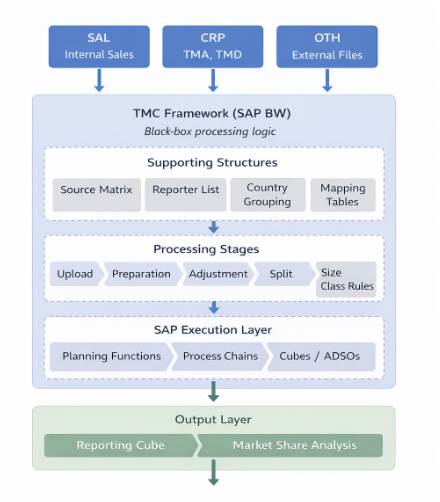
\includegraphics[width=0.9\textwidth]{tmc_architecture.png}
%     \caption{Overview of the SAP-based TMC framework and its main components.}
%     \label{fig:tmc_overview_architecture}
% \end{figure}




% \subsection{Data Sources and Supporting Structures}
% \label{subsec:tmc_data_sources}

% The TMC framework relies on three main categories of input data:

% \begin{itemize}
%     \item \textbf{SAL}: Volvo CE's internal sales data, serving as the authoritative source for its own sales volumes.
%     \item \textbf{CRP}: Statistical exchange data from the industry reporting environment, where \textit{TMA} provides the baseline estimate of the total market.
%     \item \textbf{OTH}: Externally uploaded data used to extend market coverage in cases where CRP reporting is incomplete.
% \end{itemize}

% To ensure comparability across these heterogeneous datasets, the framework depends on several supporting structures:

% \begin{itemize}
%     \item \textbf{Country grouping matrix}, used for aggregating data across geographical regions.
%     \item \textbf{Source matrix}, defining primary and secondary data sources for each market segment.
%     \item \textbf{Mapping tables}, standardizing brand and machine line classifications.
%     \item \textbf{Reporter list}, identifying which brands are treated as reporting entities.
%     \item \textbf{Size-class configuration rules}, ensuring consistency in size-based data processing and validation.
% \end{itemize}


% These supporting structures govern how records are interpreted and processed within the TMC workflow. In particular, the source matrix determines whether records proceed to subsequent calculation stages, while the reporter list influences whether records follow split-related logic or alternative processing paths.





% \subsection{Calculation Logic and SAP Execution} \label{subsec:tmc_calculation_logic} The TMC calculation follows a structured sequence of steps executed in SAP BW through Analysis for Office workbooks, upload interfaces, process chains, planning functions, and planning cubes. External file data is first uploaded and cleaned, CRP-based data is loaded through dedicated SAP processes, and the main TMC calculation is then executed on planning cubes. Final outputs are subsequently transferred to a reporting cube. The main calculation logic can be summarized as follows:

% \begin{itemize} \item \textbf{OTH upload and preprocessing:} External data is uploaded through an Analysis for Office workbook. The system validates the input structure, checks master data, and updates brand and machine-line mappings when necessary. The uploaded data is stored in an interface layer before being loaded into the analytical environment. \item \textbf{CRP upload:} CRP-based inputs, including TMA and SAL, are loaded through dedicated upload processes and consolidated into the TMC calculation environment.

% \item \textbf{Preparation -- CRP processing:} CRP data is processed first. Source-related flags, reporter distinctions, and intermediate reference values are derived. Volvo-related and non-Volvo market values are established here and reused in later split and restatement logic.

% \item \textbf{Preparation -- OTH processing:} OTH data is processed after CRP, since it depends on the reference values derived earlier. Source logic and reporter status are applied, and Volvo-related OTH records are excluded, as internal sales data is the authoritative source for Volvo CE's own volumes. 

% \item \textbf{Non-VCE total market calculation:} The non-VCE total market is derived as the difference between the overall market baseline and the Volvo-related portion, and is subsequently used as a proportional reference in later steps. 

% \item \textbf{Adjustment:} An adjustment value is calculated to keep the sum of FID values aligned with the total market baseline. Simultaneously, Volvo-related values from external market detail data are replaced by the corresponding internal sales values. This step acts both as a balancing mechanism and as a source-priority correction. 

% \item \textbf{Split:} Certain OTH records are available only in aggregated size-class structures that do not match the internal classification. These values are redistributed into finer segments using non-VCE total market values as the proportional reference, applied hierarchically from country to region to country-group level.

% \item \textbf{Total market construction:} All relevant records are consolidated, duplicate brand occurrences are removed, Volvo-related values are aligned with internal sales data, and the final total market is calculated by summing the remaining valid FID values. 

% \item \textbf{Restatement and reporting:} Selected values are recalculated proportionally to remain aligned with the reconstructed total market. The resulting dataset is transferred to the reporting layer for final market share analysis. \end{itemize}













% \begin{figure}
%     \centering
%     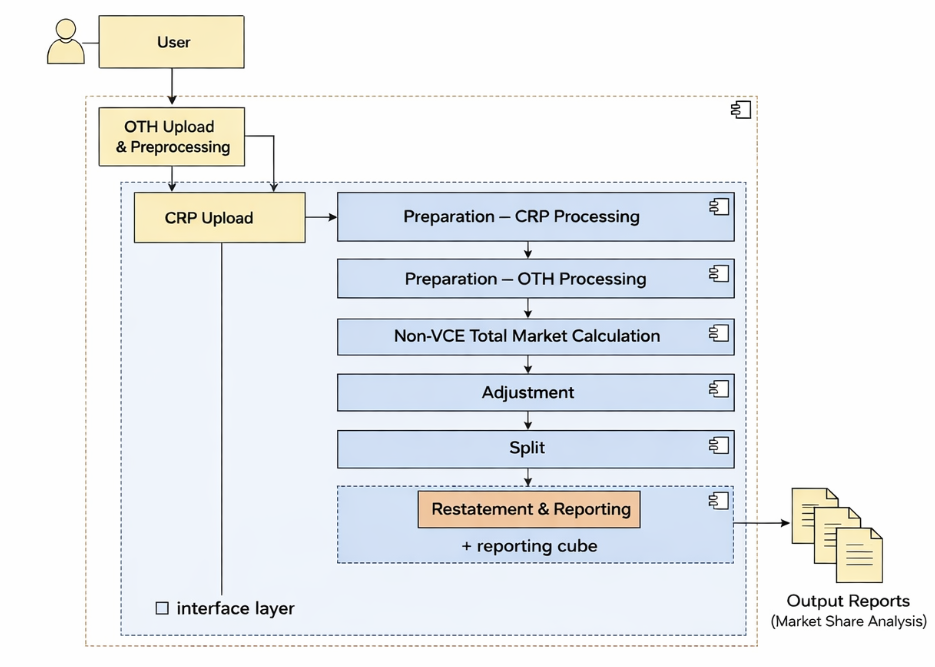
\includegraphics[width=0.9\linewidth]{tmc.png}
%     \caption{Execution flow of the SAP-based TMC framework from data upload to reporting}
%     \label{fig:tmc}
% \end{figure}







% The split step is particularly important because some external inputs are reported only in broader categories and must be translated into the finer classification required by the TMC framework. This redistribution uses the non-VCE total market structure as reference and is followed by a re-split validation step, in which implausible brand--size-class combinations are removed and remaining values are reallocated. This logic applies to reporter brands; non-reporters must already be uploaded in an appropriate size-class structure.

% For example, if an OTH record for a reporter brand is only available in the aggregated category $\text{CEX}_{\text{<10T}}$, the framework redistributes this value into $\text{CEX}_{\text{<6T}}$ and $\text{CEX}_{\text{6<10T}}$ using the non-VCE total market structure as reference. If a resulting brand--size-class combination is invalid according to the size-class configuration, it is removed and the remaining value is reallocated during the re-split step.

% Examples of typical split rules are shown below:

% \[
% \text{CEX}_{\text{<10T}} \rightarrow \{\text{CEX}_{\text{<6T}}, \text{CEX}_{\text{6<10T}}\}
% \]
% \[
% \text{GEC}_{\text{>6T}} \rightarrow \{\text{GEC}_{\text{6<10T}}, \text{GEC}_{\text{>10T}}\}
% \]
% \[
% \text{GEW}_{\text{>6T}} \rightarrow \{\text{GEW}_{\text{6<11T}}, \text{GEW}_{\text{>11T}}\}
% \]

% % \[
% % \text{WLO}_{\text{<10}} \rightarrow \{\text{WLO}_{\text{<7}}, \text{WLO}_{\text{7<10}}\}
% % \]



% \begin{figure}
%     \centering
%     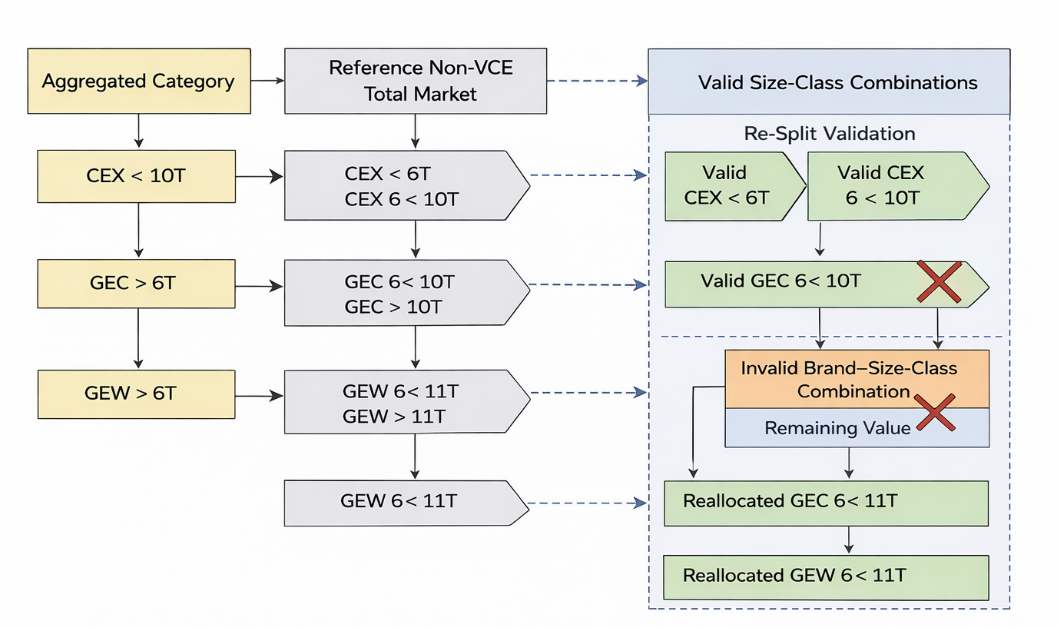
\includegraphics[width=0.9\linewidth]{split.png}
%     \caption{Illustration of split and re-split logic for aggregated OTH size-class categories.}
%     \label{fig:split}
% \end{figure}









% Overall, the SAP-based TMC framework can be understood as a layered reconstruction process in which source precedence, reporter classification, balancing adjustments, proportional redistribution, and controlled aggregation contribute to the final market share output. While analytically powerful, much of the logic is embedded inside SAP execution flows, making intermediate transformations less transparent to business users.










% 4.6.2026
% \section{Enterprise Implementation of Market Share Estimation at Volvo CE}
% \label{subsec:enterprise_tmc_volvo}

% To address the challenges of integrating heterogeneous market-related data and producing a consistent estimate of total market size, large manufacturers often implement dedicated calculation frameworks within enterprise systems. At Volvo CE, this is realized through a Total Market Calculation (TMC) framework implemented in an SAP-based analytical environment. The framework integrates multiple data sources, applies rule-based transformations, and generates the outputs used for market reporting and market share analysis.

% \subsection{ERP Systems and SAP as the Analytical Environment}

% Enterprise resource planning (ERP) systems are widely used to manage and integrate business data across organizational functions, thereby providing a foundation for analytical processes in industrial contexts \\cite{davenport1998,klaus2000}. Rather than treating business data as isolated records in separate applications, ERP systems consolidate operational information into a shared enterprise environment, making it possible to coordinate processes and reuse data across multiple business functions.

% Within the broader SAP landscape, analytical processing is typically separated from transactional business processing. ERP systems generate and consolidate operational data, whereas SAP Business Warehouse (BW) structures and provides this data for analytical use, including reporting, modeling, and transformation \cite{sap_bw4hana_guide}. BW can therefore be understood as the analytical layer of the SAP ecosystem, on top of which more complex workflows, such as market share calculation, can be implemented.

% From a technical perspective, SAP provides several components relevant to this type of calculation, including data input and loading mechanisms, analytical storage objects, multidimensional modeling structures, processing logic, and reporting outputs \cite{sap_analysis_office_guide, sap_bw_ip_overview}. Data enters the system through controlled upload and loading mechanisms, is stored in analytical structures such as InfoProviders, and is then processed through planning logic before being exposed to reporting layers.

% Two capabilities are particularly important for market share calculation. First, SAP BW organizes analytical data in a multidimensional structure rather than as flat records. In the classical BW model, an InfoCube follows SAP's enhanced star schema, in which a central fact table stores key figures and surrounding dimension tables store characteristics \cite{sap_enhanced_star_schema}. This makes it possible to analyze the same measures across multiple business perspectives. For market share calculation, this is essential because key figures such as sales volume, market volume, and market share must be structured consistently across dimensions such as country, machine line, brand, size class, and time.

% Second, SAP provides an execution layer through planning functions and planning sequences. SAP states that planning functions allow system-based processing or generation of data, while planning sequences group multiple planning functions and execute them sequentially \cite{sap_bw_ip_overview, sap_planning_sequences}. Rather than calculating market share in a single static query, SAP makes it possible to break the process into ordered operations such as copying, recalculation, deletion, distribution, and formula-based transformation \cite{sap_bw_ip_overview, sap_planning_functions}. In addition, SAP Analysis for Office enables such planning objects to be triggered through Excel-based planning front ends, where users work with input-ready analytical data and execute planning logic from a spreadsheet interface \cite{sap_analysis_office_guide}.

% Together, these capabilities provide the technical basis for implementing market share calculation in a structured and scalable enterprise environment. At Volvo CE, they support the TMC framework used to reconstruct the total market from multiple heterogeneous data sources.


\section{Enterprise Implementation of Market Share Estimation at Volvo CE}
\label{subsec:enterprise_tmc_volvo}

To understand how this broader problem appears in a real organizational setting, this thesis uses Volvo CE as a case study. Because market share estimation involves integrating heterogeneous data and applying repeatable rules across multiple business dimensions, firms may choose to implement such workflows in enterprise systems rather than rely only on isolated spreadsheets or ad hoc scripts. In the Volvo CE case, this is realized through a Total Market Calculation (TMC) framework implemented in SAP for market reporting and market share analysis.

\subsection{SAP as the Analytical Environment in the Volvo CE Case}

% Within the SAP landscape, analytical processing is typically separated from transactional business processing. ERP systems generate and consolidate operational data, whereas SAP Business Warehouse (BW) structures and provides this data for analytical use, including reporting, modeling, and transformation \cite{sap_bw4hana_guide}. BW can therefore be understood as the analytical layer of the SAP ecosystem, on top of which more complex workflows, such as market share calculation, can be implemented.

% From a technical perspective, SAP provides several components relevant to this type of calculation, including data input and loading mechanisms, analytical storage objects, multidimensional modeling structures, processing logic, and reporting outputs \cite{sap_analysis_office_guide, sap_bw_ip_overview}. Data enters the system through controlled upload and loading mechanisms, is stored in analytical structures such as InfoProviders, and is then processed through planning logic before being exposed to reporting layers.

% Two capabilities are particularly important for market share calculation. First, SAP BW organizes analytical data in a multidimensional structure rather than as flat records. In the classical BW model, an InfoCube follows SAP's enhanced star schema, in which a central fact table stores key figures and surrounding dimension tables store characteristics \cite{sap_enhanced_star_schema}. This makes it possible to analyze the same measures across multiple business perspectives. For market share calculation, this is especially important because key figures such as sales volume, market volume, and market share must be structured consistently across dimensions such as country, machine line, brand, size class, and time.

% Second, SAP provides an execution layer through planning functions and planning sequences. SAP states that planning functions allow system-based processing or generation of data, while planning sequences group multiple planning functions and execute them sequentially \cite{sap_bw_ip_overview, sap_planning_sequences}. Rather than calculating market share in a single static query, SAP makes it possible to break the process into ordered operations such as copying, recalculation, deletion, distribution, and formula-based transformation \cite{sap_bw_ip_overview, sap_planning_functions}. In addition, SAP Analysis for Office enables such planning objects to be triggered through Excel-based planning front ends, where users work with input-ready analytical data and execute planning logic from a spreadsheet interface \cite{sap_analysis_office_guide}.

% Together, these capabilities provide the technical basis for implementing market share calculation in a structured and scalable enterprise environment. In the case of Volvo CE, they support the TMC framework as a controlled enterprise data-processing setting for market-related data integration and calculation.


% Within the SAP landscape, analytical processing is typically separated from transactional business processing. ERP systems generate and consolidate operational data, while SAP Business Warehouse (BW) serves as the analytical layer for reporting, modeling, and data transformation \cite{sap_bw4hana_guide}. This separation enables enterprise-level analytical workflows to be implemented on top of integrated operational data.

% From a technical perspective, the implementation of market-related calculations in SAP relies on several key components:

% \begin{itemize}
%     \item \textbf{Data integration and storage:} Data is loaded through controlled upload interfaces and process chains, and stored in BW structures such as InfoProviders and planning cubes. These structures support multidimensional modeling based on SAP’s enhanced star schema, enabling consistent analysis across dimensions such as country, machine line, brand, and time \cite{sap_enhanced_star_schema}.

%     \item \textbf{Calculation and execution logic:} Business logic is implemented through planning functions and planning sequences, which execute ordered transformations such as copying, filtering, recalculation, and distribution \cite{sap_bw_ip_overview, sap_planning_sequences}. In practice, these operations are configured within SAP BW Integrated Planning and may involve underlying ABAP-based execution logic for system-level processing.

%     \item \textbf{User interaction and input:} Analysis for Office provides a spreadsheet-based front end through which users can input data, trigger planning sequences, and interact with analytical datasets \cite{sap_analysis_office_guide}.
% \end{itemize}

% Together, these components form a layered architecture in which SAP supports data integration, multidimensional storage, and rule-based execution within a unified enterprise environment. In the case of Volvo CE, this architecture provides the technical foundation for implementing the TMC framework as a structured analytical workflow.

% Within enterprise systems, analytical processing is typically separated from transactional operations. In the SAP landscape, operational data is generated and consolidated in ERP systems, while SAP Business Warehouse (BW) provides the analytical layer for reporting, modeling, and data transformation \cite{sap_bw4hana_guide}. This separation enables complex analytical workflows to be built on top of integrated enterprise data.

% From a technical perspective, SAP provides several core capabilities that support enterprise-level calculations such as market share estimation:

% \begin{itemize}
%     \item \textbf{Data integration and storage:} Data is loaded through structured upload mechanisms and process chains, and stored in BW objects such as InfoProviders and planning cubes. These structures follow a multidimensional model based on the enhanced star schema, enabling consistent analysis across dimensions such as country, product, and time \cite{sap_enhanced_star_schema}.

%     \item \textbf{Multidimensional modeling:} SAP BW organizes key figures and characteristics in a way that supports flexible aggregation and comparison across multiple business perspectives, which is essential for consistent market-related analysis.

%     \item \textbf{Execution of calculation logic:} Business logic is implemented through planning functions and planning sequences, which allow ordered, rule-based transformations such as copying, filtering, recalculation, and distribution \cite{sap_bw_ip_overview, sap_planning_sequences}. These operations are executed within the SAP environment and can be supported by underlying ABAP-based processing logic.

%     \item \textbf{User interaction and data input:} Tools such as Analysis for Office provide spreadsheet-based interfaces for data input, parameter control, and triggering calculation processes \cite{sap_analysis_office_guide}.
% \end{itemize}

% Together, these capabilities form a layered analytical environment in which data integration, storage, and rule-based processing are tightly coupled. This provides the technical foundation for implementing structured enterprise data-processing settings.



In the Volvo CE setting, SAP provides the technical environment in which the TMC process is carried out. Operational data is generated in enterprise systems, while SAP Business Warehouse (BW) provides the analytical layer for reporting, modeling, and transformation \cite{sap_bw_guide}. For this thesis, the key point is that SAP combines structured data loading, sequential rule execution, and spreadsheet-based user interaction \cite{sap_bw_ip_overview}. In the Volvo CE case, these capabilities form the technical foundation for a controlled enterprise data-processing setting, while also making the calculation logic difficult to inspect from a business-user perspective.












\subsection{The Existing TMC Process and Its SAP-based Implementation}
\label{subsec:tmc_process_implementation}

% At Volvo CE, market share estimation is implemented through an existing Total Market Calculation (TMC) framework within an SAP Business Warehouse (BW) environment. Rather than being executed as a single calculation, the framework operates as a staged analytical workflow in which supporting master data is first maintained, source data is then uploaded and processed, and final outputs are subsequently prepared for reporting.

% The framework combines several main categories of market-related data:

% \begin{itemize}
%     \item \textbf{SAL}: Volvo CE's internal sales data, representing the company's own recorded sales volumes.
%     \item \textbf{CRP}: Industry exchange data collected from the reporting environment and used as an important external input to the calculation process.
%     \item \textbf{TMA}: A market-level reference value derived from industry exchange data and used in later calculation stages.
%     \item \textbf{OTH}: Additional externally uploaded data used to complement market coverage where standard reporting is incomplete.
% \end{itemize}

% In addition to these source datasets, the framework depends on a dedicated master data maintenance layer. This layer includes supporting matrices and classification structures, such as brand-related information, country grouping, source definitions, participation settings, and size-class-related rules. These maintained structures provide the configuration basis on which subsequent uploads and calculations can be executed consistently.

% The framework combines several SAP components. Analysis for Office workbooks are used as spreadsheet-based front ends for maintaining master data and uploading external inputs. Dedicated upload processes and process chains manage the loading and movement of data across the SAP environment. The analytical data is then stored in SAP BW structures such as InfoProviders and planning cubes, where multidimensional characteristics and key figures can be processed consistently.

% The execution logic of the TMC framework is implemented through planning functions and planning sequences. These objects allow the system to perform ordered transformations on the analytical data, such as copying, filtering, recalculation, deletion, distribution, and formula-based processing. In this way, SAP provides not only the storage layer for market-related data but also the execution layer for rule-based calculation logic.

% Overall, the SAP-based TMC framework can be understood as a structured workflow consisting of master data maintenance, source data upload, staged calculation, validation, and reporting. Through this combination of configuration-driven processing and sequential execution logic, SAP enables Volvo CE to implement market share estimation in a controlled enterprise environment.




At Volvo CE, market share estimation is carried out through an SAP-based TMC implementation that combines maintained configuration data with several categories of workflow input, especially internal sales data (SAL), industry exchange data (CRP), derived total-market reference data (TMA), and supplementary external data (OTH). The process is staged rather than monolithic: master data and matrix rules are maintained first, source data is then loaded into BW structures, and calculation logic is executed through planning functions and planning sequences.

For the purposes of this thesis, three aspects of that implementation are most important. First, the process depends on maintained classification structures and mapping rules, not only on raw source files. Second, calculation is executed through sequential preparation, transformation, redistribution, and reporting stages. Third, the resulting logic is distributed across several SAP artefacts and interfaces rather than exposed as one inspectable process view. These characteristics make the Volvo CE TMC process a relevant case for studying transparency and traceability in ERP-based enterprise data processing.


\begin{figure}[H]
    \centering
    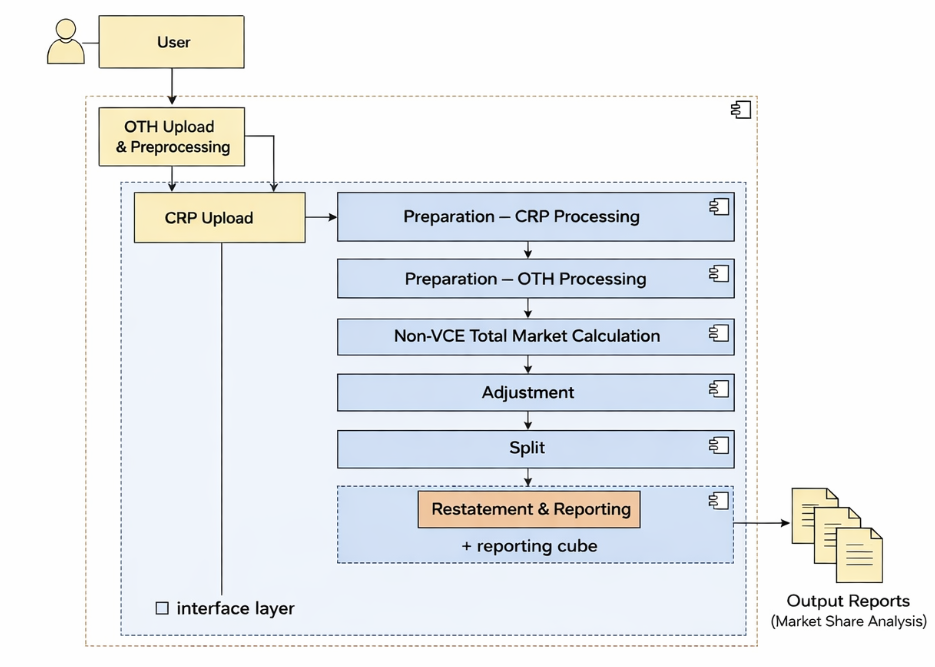
\includegraphics[width=0.9\linewidth]{tmc.png}
    \caption{Execution flow of the SAP-based TMC implementation from data upload to reporting.}
    \label{fig:tmc}
\end{figure}



\section{General Challenges in SAP-Based Enterprise Workflow Implementations}
\label{sec:sap_general_challenges}

The Volvo CE case is relevant because it reflects broader challenges that can arise when complex workflows are implemented in SAP-based enterprise environments. In such settings, business logic may be distributed across data-loading structures, maintained rules, planning objects, transformations, and reporting layers. Prior work on SAP ERP process identification highlights the difficulty of identifying relevant process structures and related tables in complex SAP environments \cite{weber2022sap}. ERP usability studies also report difficulties related to navigation, task support, presentation, and ease of use \cite{calisir2004erp,wong2016sap}.

Against that background, four general challenges are especially relevant to this thesis:

\begin{itemize}
    \item \textbf{Technical complexity:} Workflow logic may be implemented through SAP-specific objects such as planning functions, planning sequences, and other system-specific processing structures, which require specialized technical knowledge.

    \item \textbf{Limited transparency:} Processing may be executed across multiple system layers without one clear representation of the full workflow, making intermediate transformations difficult for business users to inspect and interpret.

    \item \textbf{Dependency on technical specialists:} When logic is embedded in system-specific structures, modifying, validating, or explaining workflow behavior may require technical support rather than direct business-user inspection.

    \item \textbf{Reduced traceability:} A distributed implementation can make it difficult to trace how data moves through transformations, verify intermediate results, and assess the effect of logic changes.
\end{itemize}

These broader challenges form the problem context for this thesis and are examined through the Volvo CE case study.








\section{Related Work}

To position these challenges in prior research, the literature relevant to this thesis can be grouped into three areas. First, data-warehouse and ETL literature describes enterprise analytics as staged workflows in which heterogeneous data is extracted, transformed, and prepared for reporting or decision support \cite{vassiliadis2009etl}. Related work on heterogeneous data integration shows that such workflows often involve inconsistent inputs and integration challenges \cite{putrama2024heterogeneous}. Work on data-pipeline quality similarly highlights transformation errors and related data-quality problems \cite{foidl2024pipeline}. This supports the need for explicit transformation stages and quality-control mechanisms in ERP-based enterprise data processing.

Second, ERP and SAP-related research highlights the complexity and usability challenges of enterprise systems. ERP systems integrate business processes across organisational functions \cite{klaus2000}. At the same time, that integration can introduce complex data structures, system-specific logic, and interfaces that require specialised knowledge \cite{davenport1998}. Research on SAP ERP process extraction shows that identifying relevant process structures and tables can be difficult in SAP environments \cite{weber2022sap}. ERP usability studies also show that navigation, task support, learnability, and output presentation affect end-user effectiveness \cite{calisir2004erp}. Similar concerns appear in SAP-related user settings \cite{wong2016sap}. These findings are relevant because the problem addressed in this thesis concerns not only workflow execution, but also whether business users can inspect and validate how outputs are produced.

Third, decision-support and enterprise analytics literature suggests that analytical functionality can be supported through additional user-facing layers that help users review data and interpret outputs \cite{march2007dss}. Work in the construction domain similarly shows that data-warehouse and decision-support layers can support analytical tasks beyond transactional enterprise systems \cite{fan2006equipmentdw}. Such layers can complement existing enterprise systems by providing more accessible interfaces for inspection, comparison, and validation.

Taken together, this literature supports the problem framing used in this thesis: ERP-based enterprise data processing can be technically robust and operationally useful while still being difficult for business users to inspect step by step. Within the literature reviewed for this thesis, no concrete browser-based design example was identified that re-expresses selected SAP-based workflow logic as explicit, reviewable stages for business users. This thesis addresses that gap through a Design Science Research study using Volvo CE's Total Market Calculation process as the empirical case study, while framing the underlying problem as a broader ERP-based enterprise data-processing challenge.

























% !TEX root = ../Thesis.tex
\chapter{Methodology} \label{cha:method}

% \section{Choice of Research Strategy}



% \
% This thesis adopts Design Science Research (DSR) as its overall research framework. Design Science Research (DSR) is a research framework concerned with the design and evaluation of artefacts intended to address practical problems \cite{johannesson2021,hevner2004design}. In information systems research, DSR is particularly relevant when the aim is not only to solve a real-world problem, but also to generate design knowledge through the artefact development process \cite{gregor2013}. 

% This research fits that orientation well. Rather than only analyzing the limitations of the existing SAP-based TMC implementation at Volvo CE, the thesis aims to design and implement a web-based prototype that improves transparency, usability, and traceability in the preparation and adjustment stages. The study therefore focuses on creating an artefact that addresses a concrete industrial problem and examining its usefulness in practice.

% To structure the research process, the thesis follows the five core DSR activities proposed by Johannesson and Perjons: explicate the problem, define requirements, design and develop the artefact, demonstrate the artefact, and evaluate the artefact \cite{johannesson2021,hevner2004design}. In this thesis, these activities provide a systematic structure for moving from problem understanding to requirement definition, prototype development, and formative evaluation in the Volvo CE context.

% The five activities applied in this thesis are summarized as follows:

% \begin{itemize}
%     \item \textbf{Explicate the problem}: identify and clarify the limitations of the current TMC workflow and the needs of potential users.
%     \item \textbf{Define requirements}: derive functional and non-functional requirements for the prototype based on workflow analysis, documentation, and stakeholder needs.
%     \item \textbf{Design and develop the artefact}: design and implement a web-based frontend-backend prototype for data upload, workflow navigation, calculation-layer visualization, and interactive table analysis.
%     \item \textbf{Demonstrate the artefact}: apply the prototype to representative TMC-related data and workflow scenarios to show its practical usefulness.
%     \item \textbf{Evaluate the artefact}: assess whether the prototype improves visibility, usability, and interpretability of the preparation and adjustment stages.
% \end{itemize}

% Using DSR makes it possible to connect practical system development with academic research in a structured way. It provides a methodological basis for both building the prototype and reflecting on its contribution as a reusable approach for improving workflow transparency in enterprise data-processing systems.


% \subsection{Choice of Research Framework}

% Design Science Research (DSR) is a research strategy concerned with the design and evaluation of artefacts intended to address practical problems in real-world contexts \cite{johannesson2021,hevner2004design}. This thesis adopts DSR as its overall research framework, as the study aims not only to examine limitations in the existing SAP-based Total Market Calculation (TMC) workflow at Volvo CE, but also to design and evaluate a prototype that improves its transparency, usability, and traceability.

% DSR is particularly suitable for this thesis because the main contribution is an artefact rather than a purely descriptive account of the current workflow. While approaches such as case study are useful for understanding organizational settings and existing practices, they do not by themselves provide a structured process for developing and evaluating a technical solution. In contrast, DSR offers a systematic way to move from problem identification to requirement definition, artefact design, demonstration, and evaluation \cite{johannesson2021,hevner2004design}.

% In this thesis, the artefact is a web-based prototype that reconstructs and visualizes selected preparation and adjustment stages of the TMC workflow outside the original SAP environment. The purpose of the prototype is to make key transformations, data dependencies, and intermediate outputs easier to inspect and understand. In this way, the artefact addresses a practical industrial problem while also providing knowledge about how workflow transparency can be improved in enterprise data-processing systems.

% To structure the research process, the thesis follows the five core DSR activities proposed by Johannesson and Perjons: explicate the problem, define requirements, design and develop the artefact, demonstrate the artefact, and evaluate the artefact \cite{johannesson2021,hevner2004design}. In the present study, these activities provide a clear methodological structure for moving from understanding the limitations of the current TMC process to developing and assessing a prototype in the Volvo CE context.


% \section{Research Strategy}

Design Science Research (DSR) was selected because this thesis was not limited to describing the existing SAP-based TMC implementation. The main task was to build an artefact, apply it to realistic case material, and evaluate whether it made selected process stages easier to inspect \cite{johannesson2021,hevner2004design}. In DSR terms, the artefact is the proposed inspection-oriented solution, while the implemented prototype is its concrete instantiation in this thesis. This orientation fits the study because the intended contribution is partly practical and partly explanatory: the work needed to solve a real workflow-inspection problem, but also to show what kind of design choices made that solution useful in context.

The work followed the five DSR activities described by Johannesson and Perjons \cite{johannesson2021}, but not as a rigid linear sequence. Problem understanding, requirement clarification, implementation, and evaluation informed each other during the project. In practice, this mattered because several parts of the workflow could not be understood from documentation alone. As prototype outputs became available, they also revealed ambiguities that had to be discussed again with stakeholders before later stages could be implemented with confidence.

This thesis combines Design Science Research (DSR) with a case study. \textbf{Alternative research methods.} A stand-alone \textbf{case study} would have been appropriate for describing the organizational setting and the existing workflow \cite{yin2018}, but this thesis also required artefact design and evaluation. \textbf{Action research} was less suitable because the project did not aim to intervene directly in Volvo CE's live production process \cite{susman1978}. More measurement-oriented approaches, such as \textbf{surveys} or \textbf{controlled experiments}, were also less suitable because the work depended on a small group of knowledgeable stakeholders and on detailed interpretation of workflow logic.

The broader design problem concerns transparency, traceability, and usability in ERP-based enterprise data processing, but it was studied through one concrete setting: the TMC process at Volvo CE. Within the overall DSR design, the Volvo CE setting functioned as a case study used to understand the workflow problem in context, guide artefact design, and assess the implemented prototype in a real organizational environment.



% \section{Application of the Design Science Research Framework}
\section{Research Method}


% This thesis used a combination of qualitative and technical data collection methods across the five DSR activities. DSR supports the development and evaluation of artefacts in response to practical problems, while allowing different empirical methods to be used depending on the purpose of each activity \cite{johannesson2014introduction,hevner2004design}. Since the study was conducted in a specialised organisational context, document review, workflow inspection, stakeholder discussions, and prototype-based feedback were used as the main data collection methods. These methods are suitable for small-scale qualitative research where the aim is to obtain contextual and practice-oriented understanding rather than broad statistical generalisation \cite{denscombe2017good}.

% In the problem explication stage, data were collected through review of TMC-related documentation, inspection of the existing SAP-based implementation, and informal discussions with stakeholders in Volvo CE Global Business Intelligence. These sources were used to understand the limitations of the current workflow, particularly the lack of transparency, traceability, and inspectability in intermediate calculation steps. In the requirements definition stage, additional data were collected from workflow documentation, source data structures, matrix files, example outputs, and stakeholder input. This helped translate the identified problem into functional, structural, and environmental requirements for the artefact.

% During the design and development stage, data collection focused on technical material needed to reconstruct selected parts of the TMC workflow. This included CSV-based source files, matrix tables, mapping rules, and selected SAP-related workflow descriptions. Clarifications were also collected through stakeholder discussions when calculation rules or data dependencies required further interpretation. In the demonstration stage, the artefact was applied to a realistic TMC workflow scenario using 2024 source data and matrix files. The generated preparation, market view, adjustment, machine line split, and resplit outputs were used to demonstrate how the prototype could make intermediate workflow layers more inspectable. Finally, in the evaluation stage, data were collected through prototype-based stakeholder feedback, semi-structured discussion, output inspection, and requirement-based review.

% Alternative data collection methods were also considered. Large-scale surveys, focus groups, formal requirements workshops, direct SAP backend extraction, production-system integration, and full operational pilot deployment could have been used. However, these methods were less suitable for the scope of this thesis. The TMC workflow is a specialised internal process involving a limited number of knowledgeable users, and the artefact was developed as a research prototype outside the production SAP environment. Therefore, qualitative and technical data collection methods were considered more appropriate than broad survey-based or production-level methods.

% \subsection{Data Collection Methods}

This thesis used three main sources of empirical material: \textbf{document analysis}, \textbf{stakeholder clarification and feedback sessions}, and \textbf{prototype-based material}. To understand the TMC process, it was necessary to review workflow descriptions, source files, and matrix structures, but some rule interpretations still depended on business context.

Document analysis was therefore used to examine process materials, workflow descriptions, source data structures, and matrix files \cite{bowen2009document}. The document set was limited to materials directly relevant to the studied 2024 TMC workflow and the implemented stages. Outdated versions, unrelated SAP reports, and partial notes that could not be connected to the selected workflow scope were not treated as primary analytical material. This helped keep the analysis close to the actual workflow represented in the artefact, rather than drifting into broader SAP material that was not operationally relevant for the case. When documents conflicted or left rule details unclear, stakeholder clarification and output comparison were used to resolve the interpretation.

Recurring weekly review meetings and related clarification discussions were used to clarify business rules, expected outputs, and gaps in the documentation. These interactions were not conducted as a formal interview study. Instead, they functioned as case-based clarification and feedback sessions within the broader DSR and case study design. To avoid relying only on individual interpretations, unclear points were checked against documents, source structures, matrix definitions, and generated outputs wherever possible. Prototype-based material was then collected during design, demonstration, and evaluation in the form of uploaded inputs, generated outputs, result comparisons, and stakeholder comments \cite{runeson2009guidelines}.





% \subsection{Data Analysis Method}

The collected material was analysed through a combination of \textbf{qualitative interpretation} and \textbf{technical inspection}. In practice, this meant breaking the workflow into stages, interpreting rules from documents and stakeholder explanations, checking how those rules appeared in prototype outputs, and comparing implemented results with expected behaviour \cite{johannesson2021,hevner2004design}. The study was not conducted as a formal line-by-line content analysis. Instead, the main unit of analysis was the \textit{workflow stage} together with its associated inputs, rules, transformations, and generated outputs.

The analytical categories were mainly deductive. Transparency, traceability, usability, validation support, and requirement fulfilment were derived from the research problem, related work, and the DSR purpose of the study. At the same time, the analysis remained open to case-specific issues such as unclear rule ownership, reference-data version differences, and stage-specific inspection needs. Accordingly, the analysis should be understood as structured workflow analysis in a DSR case study rather than as an inductive code-to-theme thematic analysis.

During problem explication and requirements definition, the analysis focused on understanding where business users lost visibility in the existing process and which functions would be most useful in an inspection-oriented prototype. During design and development, the analysis became more concrete: source files, mapping tables, matrix rules, and workflow descriptions were examined to determine how selected SAP-based logic could be reconstructed as explicit processing steps. During demonstration and evaluation, the generated outputs were inspected stage by stage and compared with expected workflow behaviour and selected reference outputs. Stakeholder feedback was reviewed qualitatively, especially comments about whether the prototype made it easier to understand a stage, inspect an intermediate result, or discuss an unexpected value.







\section{Application of the Research Method}

This section summarizes how the selected data collection and analysis methods were applied across the five DSR activities. Detailed artefact design, implementation, demonstration, and evaluation are presented in later chapters.

\subsection{Explicate the Problem}

The first DSR activity was to explicate the problem. This was done by reviewing workflow descriptions, source structures, matrix files, existing SAP-based outputs, and stakeholder explanations in order to understand where business users lost visibility in the current TMC process. The goal was not only to describe how the workflow runs, but to identify where input dependencies, transformation logic, and intermediate results became difficult to inspect.

The collected material was analysed through qualitative interpretation of the workflow steps and technical inspection of how data and rules were distributed across the existing implementation. This made it possible to frame the problem more precisely as one of transparency, traceability, and usability in a staged enterprise data-processing workflow rather than as a single isolated system defect.

\subsection{Define Requirements}

The second DSR activity was to define requirements for the artefact. Workflow documentation, source data structures, matrix files, existing output examples, and stakeholder input were used to clarify what the prototype needed to support. The purpose was to translate the identified workflow problems into concrete requirements for a web-based artefact.

The collected material was analysed through requirements analysis. The requirements were grouped into functional and performance requirements. Functional requirements described capabilities such as file upload, backend processing, structured storage, intermediate output inspection, filtering, validation support, and export. Performance requirements addressed prototype-level execution time, stability, and reliability during demonstration and evaluation.

The resulting requirements guided the design and development of the prototype and provided the basis for the requirement-based evaluation in Chapter 6, where the artefact is assessed in terms of functional coverage, transparency, traceability, usability, validation support, and prototype-level performance.

















% The third activity of the DSR framework is to design and develop the artefact. This activity takes the outlined artefact and the elicited requirements as input and transforms them into a concrete implementation. According to Johannesson and Perjons, this activity can be understood through four sub-activities: imagine and brainstorm, assess and select, sketch and build, and justify and reflect \cite{johannesson2021,hevner2004design}. In this thesis, the activity was carried out through a combination of iterative prototyping, workflow analysis, and discussions with relevant stakeholders in the Volvo CE context.

% The first sub-activity, \textit{imagine and brainstorm}, involved exploring how the TMC workflow could be represented in a more transparent and user-friendly way outside the current SAP-based environment. Early ideas focused on how source data upload, workflow navigation, intermediate layer inspection, and calculation-related views could be presented through a web-based interface. These ideas were developed through technical analysis of the workflow and informal discussions with stakeholders involved in business intelligence and market-related analysis.

% The second sub-activity, \textit{assess and select}, involved evaluating alternative design directions and selecting the ones most suitable for the scope of the thesis. A web-based prototype was chosen rather than a script-based or spreadsheet-based solution, as it provided better support for structured navigation, interactive data inspection, and future internal use within Volvo CE. In addition, a frontend-backend architecture was selected in order to separate user interaction from backend processing and data handling. The implementation scope was defined up to the machine line split stage, while the preparation and adjustment stages were given particular emphasis in the thesis.

% The third sub-activity, \textit{sketch and build}, involved translating the selected design into a working prototype. The artefact was implemented as a web-based system with dedicated views for authentication, homepage navigation, source data upload, and workflow layer inspection. Uploaded CSV-based files were processed through backend services and stored in a local relational database, allowing selected parts of the workflow logic to be re-expressed through Python- and SQL-based processing in a more inspectable form than in the original SAP environment. The prototype was developed iteratively, and different parts of the system were refined as the understanding of the workflow and its representation evolved.

% The fourth sub-activity, \textit{justify and reflect}, involved reviewing the design decisions against the defined requirements. During development, features such as workflow-layer navigation, interactive filtering, summary calculation, and CSV export were assessed not only as interface functions, but also as responses to the identified lack of transparency, traceability, and usability in the original workflow. This reflection also helped identify possible directions for future development, including support for additional workflow stages and tighter integration with Volvo CE internal infrastructure.

% A key design decision in this thesis was to represent selected parts of the TMC workflow through a modular web-based prototype rather than attempt to replicate the SAP environment directly. Another important decision was to externalize selected workflow logic through backend services and SQL-based data handling, instead of relying on SAP-specific execution structures. This made the preparation, market view, adjustment, machine line split, and resplit-related logic easier to inspect and explain, while remaining manageable within the scope of the thesis.

% One challenge encountered during development was how to represent the complexity of the TMC workflow in a simplified but still meaningful way. The original SAP-based process involves multiple data sources, matrix-based business rules, and staged transformations. To make the artefact feasible within the thesis, the implementation was limited to workflow coverage from source data upload to machine line split, while preserving the essential logic needed to demonstrate the value of a more transparent and user-oriented representation.

% \paragraph{Alternative strategy}
% An alternative strategy would have been to develop the artefact through action research in closer integration with ongoing organizational processes. However, this was not chosen because the thesis was conducted in an exploratory mode and did not aim to introduce changes directly into the production environment. An iterative prototyping strategy combined with stakeholder feedback was therefore more suitable for developing and refining the artefact in this context.

% \subsection{Design and develop artifact}

% The third activity of the DSR framework is to design and develop the artefact, transforming the outlined artefact and elicited requirements into a concrete implementation. According to Johannesson and Perjons, this activity can be understood through four sub-activities: imagine and brainstorm, assess and select, sketch and build, and justify and reflect \cite{johannesson2021,hevner2004design}.

% The first sub-activity, \textit{imagine and brainstorm}, concerned how the TMC workflow could be represented in a more transparent and user-friendly way outside the SAP-based environment. Early ideas focused on data upload, workflow navigation, intermediate layer inspection, and calculation-related views.

% The second sub-activity, \textit{assess and select}, required evaluating alternative design directions. A web-based prototype was chosen over a script-based or spreadsheet-based solution, and a frontend-backend architecture was selected to separate user interaction from backend processing. The implementation scope was defined up to the machine line split stage.

% The third sub-activity, \textit{sketch and build}, translated these decisions into a working prototype. Uploaded CSV-based files were processed through backend services and stored in a local relational database, allowing selected workflow logic to be re-expressed through Python- and SQL-based processing in a more inspectable form than in the original SAP environment. The prototype was developed iteratively as the understanding of the workflow evolved.

% The fourth sub-activity, \textit{justify and reflect}, involved reviewing the design decisions against the defined requirements and checking whether the prototype produced results consistent with the intended workflow logic. Using 2024 TMC source data and matrix files, selected outputs were spot-checked against the defined calculation rules. This helped assess the correctness of the reformulated backend logic and identify remaining limitations of the artefact.




% A key design decision was to represent selected parts of the TMC workflow through a modular web-based prototype rather than attempt to replicate the SAP environment directly. Another was to externalize selected workflow logic through backend services and SQL-based data handling instead of relying on SAP-specific execution structures.

% One challenge during development was translating calculation logic embedded in the SAP environment into executable backend logic. In the original system, important workflow steps are expressed through planning functions, planning sequences, matrix-based structures, and staged transformations, none of which map directly onto reusable code. These structures had to be interpreted and reformulated into Python- and SQL-based processing logic. To keep the artefact feasible within the scope of the thesis, the implementation was limited to workflow coverage from source data upload to machine line split.

% \paragraph{Alternative strategy} An alternative strategy would have been to develop the artefact through action research in closer integration with ongoing organizational processes. However, given that the thesis was conducted in an exploratory mode without the aim of introducing changes into the production environment, iterative prototyping combined with stakeholder feedback was the more suitable approach.

\subsection{Design and Develop the Artefact}

The third DSR activity was to design and develop the artefact based on the requirements defined in the previous activity. Since the main contribution of this thesis is a working prototype, this activity formed a central part of the research process \cite{johannesson2021,hevner2004design}.

In this stage, CSV-based source files, matrix tables, mapping rules, workflow descriptions, and generated outputs were inspected to understand how selected parts of the workflow could be reconstructed outside the SAP environment. Stakeholder clarification was used when business rules, machine-line mappings, or data dependencies were unclear. The collected material was analysed through workflow decomposition, rule interpretation, and iterative output inspection, which supported the translation of selected workflow logic into explicit Python- and SQL-based backend processing steps.

The development followed an iterative prototyping approach. Early design ideas focused on staged outputs, workflow navigation, filtering, summary values, and export functions. These ideas were gradually implemented and refined as understanding of the workflow improved. The implemented scope covered source data upload, preparation, market view, adjustment, machine line split, and resplit. A key challenge was that important workflow logic in the original SAP-based process is embedded in planning functions, planning sequences, matrix-based structures, and staged transformations, so it had to be interpreted and reformulated into backend processing logic. The iterative approach was therefore not only a practical way of building software, but also a way of learning the workflow itself: each implemented stage made it easier to see what data, rule assumptions, and inspection needs had to be represented next.




% \subsection{Demonstrate artefact}





% The fourth activity of the DSR framework is to demonstrate the artefact. This activity shows how the artefact can be applied in a relevant case to address the previously explicated problem. In this sense, the demonstration serves as a proof of feasibility for the artefact \cite{johannesson2021,hevner2004design}.

% The first sub-activity was to choose a case on which to apply the artefact. In this thesis, the demonstration was based on a realistic TMC workflow scenario using 2024 TMC source data and matrix files. The case focused on how users could upload workflow-related input data, process it through the implemented stages, and inspect the resulting preparation-, adjustment-, and split-related outputs in the prototype.

% The second sub-activity was to apply the artefact to the selected case. The uploaded CSV-based source data and matrix files were processed through the backend, where selected workflow logic was handled through Python-based services and SQL-backed data processing. The resulting outputs were then made available in the web interface through layer-based views, interactive tables, summary calculations, and CSV export functionality.

% This demonstration showed that the artefact could be used to support the workflow from source data upload to machine line split in a more transparent and inspectable way than the corresponding SAP-based representation. It therefore served as a proof of concept for the feasibility of the proposed web-based prototype.

% \paragraph{Alternative strategy}
% An alternative strategy would have been a broader pilot deployment in an ongoing Volvo CE workflow. However, this was not chosen because the thesis focused on demonstrating the feasibility of the prototype in a realistic use case rather than introducing it into wider operational use.

% \subsection{Demonstrate the Artefact}

% The fourth DSR activity was to demonstrate the artefact. This activity shows how the artefact can be applied in a relevant case and can serve as a proof of feasibility for the proposed solution \cite{johannesson2021,hevner2004design}. In this thesis, the demonstration was based on a realistic TMC scenario using Volvo CE's 2024 market data and matrix files used for the yearly TMC calculation.

% The selected data collection methods were applied by using the prototype to upload source and matrix files, process them through the implemented backend stages, and generate outputs for preparation, market view, adjustment, machine line split, and resplit. These outputs were then made available through the web interface using layer-based views, interactive tables, summary values, charts, and CSV export functions.

% The demonstration focused on showing how users could follow selected workflow stages step by step, inspect intermediate outputs, and review results through the prototype interface. In this way, the activity demonstrated the feasibility of representing selected parts of the TMC workflow outside the SAP environment in a more transparent and inspectable form.

% The detailed demonstration of the prototype and its generated workflow outputs is presented in the results chapter.


% \subsection{Demonstrate the Artefact}

% The fourth DSR activity was to demonstrate the artefact. This activity shows how the artefact can be applied in a relevant case and can serve as a proof of feasibility for the proposed solution \cite{johannesson2021,hevner2004design}. In this thesis, the demonstration was based on a realistic TMC scenario using Volvo CE's 2024 market data and matrix files used for the yearly TMC calculation.

% The selected data collection methods were applied by using the prototype to upload source and matrix files, process them through the implemented backend stages, and generate preparation, market view, adjustment, machine line split, and resplit outputs. These outputs were then made available through the web interface using layer-based views, interactive tables, summary values, and CSV export functions.

% The generated outputs were analysed through structured output inspection and comparison with the expected workflow logic. In particular, the results were checked against the defined business rules, expected intermediate outputs, and, where comparable, the results produced by the existing SAP-based TMC implementation. This helped assess whether the reformulated backend logic behaved consistently with the intended TMC process within the implemented scope.

% This activity served as a proof of feasibility for the artefact within the selected scope, from source data upload to machine line split. The detailed demonstration, output inspection, and comparison results are presented in the results and evaluation chapters.


\subsection{Demonstrate the Artefact}

The fourth DSR activity was to demonstrate the artefact. This activity shows how the artefact can be applied in a relevant case and can serve as a proof of feasibility for the proposed solution \cite{johannesson2021,hevner2004design}. In this thesis, the artefact was demonstrated through the Volvo CE case study using a realistic TMC scenario with 2024 market data and matrix files.

The prototype was used to upload source and matrix files, process them through the implemented backend stages, and generate outputs for preparation, market view, adjustment, machine line split, and resplit processing. These outputs were made available through the web interface using layer-based views, interactive tables, summary values, charts, and CSV export functions. The activity therefore demonstrated the feasibility of representing selected parts of the workflow outside the SAP environment in a more transparent and inspectable form.

The detailed demonstration of the prototype and its generated workflow outputs is presented in the results chapter.



% \subsection{Evaluate Artefact}
% The final activity of the DSR framework is to evaluate the artefact. This activity aims to determine whether the artefact fulfils its intended purpose and satisfies the previously defined requirements.\cite{johannesson2021} In this thesis, the artefact was evaluated through prototype use, output inspection, and stakeholder feedback.

% The first sub-activity was to analyse the evaluation context. The evaluation was carried out using the deployed web-based prototype, which was made accessible to stakeholders through a test deployment. Representative 2024 TMC source data and matrix files were used as input. The setting was realistic in terms of data and workflow context, but still limited to the current prototype scope.

% The second sub-activity was to select evaluation goals and strategy. The main goals were to assess whether the artefact improved transparency, usability, and inspectability compared with the SAP-based TMC implementation, and whether it fulfilled the defined requirements. Since the artefact had not yet been introduced into broader internal use, the evaluation was formative and qualitative in nature.

% The third sub-activity was to design and carry out the evaluation. A feedback session was conducted with a small group of two to three stakeholders from Volvo CE, including personnel from the Strategy and Business Intelligence team responsible for market research and the yearly TMC cycle. Stakeholders accessed the deployed prototype directly through a test environment and interacted with the system using real workflow data. Feedback was collected through semi-structured discussion following the session.

% The evaluation indicated that the artefact improved workflow visibility and made intermediate results easier to inspect compared with the SAP-based process. Stakeholders found the web-based interface easier to operate than the existing SAP environment and noted that the layer-based views provided clearer visibility into intermediate workflow steps than was previously available. The interactive filtering, summary calculation, and CSV export features were considered useful for review and validation purposes. Stakeholders also highlighted the potential for further development, in particular the extension of the prototype to cover later workflow stages such as Total Market Calculation, suggesting that the current implementation provides a solid foundation for broader future use.

% \paragraph{Alternative strategy}
% An alternative strategy would have been a broader pilot deployment within an ongoing Volvo CE workflow. However, this was not chosen because the artefact is still at the prototype stage, and a formative qualitative evaluation was more suitable for identifying improvements before wider internal use.



% \subsection{Evaluate the Artefact}

% The final DSR activity was to evaluate the artefact. This activity aimed to determine whether the prototype fulfilled its intended purpose and satisfied the requirements defined earlier in the research process \cite{johannesson2021,hevner2004design}. Since the artefact was developed as a research prototype, the evaluation was formative and qualitative rather than a full production assessment.

% In this activity, data were collected through prototype use, structured output inspection, and stakeholder feedback. The prototype was evaluated in a test setting using Volvo CE's 2024 market data and matrix files. The generated outputs were inspected to assess whether the implemented workflow stages behaved according to the defined business rules and expected workflow logic. Where comparable, selected results were also checked against the existing SAP-based TMC process.

% The collected material was analysed through requirement-based evaluation and qualitative feedback analysis. The evaluation focused on whether the artefact supported transparency, traceability, usability, validation support, and prototype-level performance within the implemented scope. Stakeholder feedback was used to understand whether the prototype made intermediate workflow stages clearer and easier to review from a user perspective.

% The detailed evaluation design, parameters, results, and limitations are presented in the evaluation chapter.



\subsection{Evaluate the Artefact}

The final DSR activity was to evaluate the artefact. This activity aimed to determine whether the prototype fulfilled its intended purpose and satisfied the requirements defined earlier in the research process \cite{johannesson2021,hevner2004design}. Since the artefact was developed as a research prototype, the evaluation was formative and qualitative rather than a full production-level assessment.

Data were collected through prototype use, structured output inspection, and stakeholder feedback. The prototype was evaluated in a test setting using Volvo CE's 2024 market data and matrix files, and the evaluation focused on the implemented workflow scope from source data upload to preparation, market view, adjustment, machine line split, and resplit.

The generated outputs were inspected to assess whether the implemented stages behaved according to the defined business rules and expected workflow logic. Where comparable, selected results were also checked against outputs from the existing SAP-based TMC process. The collected material was analysed through requirement-based evaluation and qualitative feedback analysis, with attention to functional fulfilment, prototype-level performance, transparency, traceability, usability, and validation.

The detailed evaluation parameters, results, and limitations are presented in the evaluation chapter.











\section{Ethical Considerations}

This study was conducted in collaboration with Volvo CE and required careful attention to research integrity, confidentiality, and responsible handling of research material. The study was guided by principles of good research practice, including transparency, honesty, and respect in the conduct and reporting of research \cite{su_ethics_policy}.

The empirical part of the thesis involved workflow analysis, document review, prototype development, and recurring review meetings and clarification discussions with relevant stakeholders. No sensitive personal data was collected or processed, and the study did not involve any physical intervention or any attempt to influence participants physically or mentally. Stakeholders who contributed contextual information were informed about the purpose of the study, and participation in discussions was voluntary \cite{etikprovningsmyndigheten_act}.

The purpose of these interactions was solely to understand current work practices and support the design and assessment of the artefact, not to evaluate or report individual performance or behaviour. In this way, the study sought to respect participants' autonomy while limiting the use of collected material to what was necessary for the research purpose \cite{vr_good_research_2024}.

Special consideration was also given to the handling of company-internal information. The prototype was developed and demonstrated in a controlled setting and was not used as a production replacement. Where screenshots, figures, code fragments, system outputs, or data samples from internal systems were included for explanatory purposes, they were anonymised or masked to remove company-specific identifiers and potentially sensitive information. The thesis does not disclose Volvo CE trade secrets, confidential business data, or complete proprietary calculation logic, and the handling of company-related material followed Volvo CE's internal requirements for confidentiality and responsible information handling \cite{su_ethics_policy}.

Overall, the study was conducted in accordance with Stockholm University's ethical framework, Swedish principles for good research practice, and Volvo CE's internal requirements for confidentiality and responsible information handling, with particular attention to confidentiality, responsible data handling, and respect for the individuals involved in the research context \cite{vr_good_research_2024}.





























\chapter{Problem and Requirements} \label{cha:results}
\section{Problem}

\subsection{Problem Context}

The case context of this thesis is the Total Market Calculation (TMC) workflow at Volvo Construction Equipment (Volvo CE). The workflow is currently executed in SAP and is used to calculate total market and market share values across dimensions such as country, machine line, size class, source, and brand.

The yearly TMC process depends on multiple data sources and matrix-based business rules, including Volvo CE sales data, industry-related reference data, external market data, source mapping, reporter logic, country grouping, and size-class handling. These inputs are processed through staged workflow steps such as source data upload, preparation, adjustment, and machine line split.

Although the SAP-based framework supports the required calculations, the process is difficult for business users to inspect and validate because intermediate preparation, adjustment, and split outputs are not exposed in a single review-oriented interface. Much of the workflow logic is embedded in SAP-specific technical structures, such as planning functions, planning sequences, BW objects, and matrix-driven rule configurations. As a result, users often see processed results without being able to easily follow the intermediate transformations that produced them.

\subsection{Root Cause Analysis and Design Objective}

The problem is particularly visible in the preparation, adjustment, and split stages, where TMA, SAL, CRP, OTH, and matrix-based rules are combined. Because intermediate outputs and rule applications are not presented in one coherent interface, users have limited ability to understand how values are derived, verify whether rules have been applied correctly, or identify where inconsistencies originate. In practice, this also increases dependency on Volvo internal IT for executing the workflow, interpreting SAP-specific logic, exporting intermediate results, and applying rule adjustments.

A root cause analysis identified four primary issues:
\begin{itemize}
    \item The workflow logic is embedded in SAP-specific planning functions, planning sequences, BW objects, and matrix-driven rule configurations, making it difficult to inspect outside the SAP environment.
    \item Intermediate stages such as preparation, adjustment, and split are not presented in a single coherent interface, which reduces transparency and traceability.
    \item Multiple source datasets and matrix-based rules are distributed across separate technical structures, making the relationship between inputs, rules, and outputs difficult to interpret.
    \item The yearly execution and validation of the workflow depend strongly on IT support, which increases communication effort and reduces direct control for business users.
\end{itemize}

This thesis therefore addresses the problem by designing a web-based TMC workflow inspection prototype. The prototype re-expresses selected workflow logic outside the SAP environment using SQL-backed processing and presents intermediate results through a browser-based interface. The aim is not to replace SAP, but to explore how selected stages of the TMC workflow can be made more transparent, traceable, and usable by exposing staged outputs, showing relevant rule and context fields, and supporting filtering, summary calculation, and export.












\section{Requirements}
\label{sec:requirements}


Based on the problem identified in the SAP-based TMC workflow, this thesis defines requirements for a web-based data processing and visualisation artefact. The artefact is intended to support the selected workflow scope from source data upload to preparation, adjustment, and machine line split, and to guide the later evaluation of transparency, traceability, usability, validation support, and prototype performance.

The requirements were derived from analysis of the existing SAP-based workflow, available technical documentation, and discussions with stakeholders from Volvo CE Strategy and Business Intelligence. They reflect the current execution model, data dependencies, workflow stages, and practical needs related to intermediate result inspection, rule validation, and reduced dependency on SAP-specific technical knowledge.

The requirements are grouped into two categories: functional requirements, covering upload, processing, storage, inspection, traceability, validation support, and user interaction; and performance requirements, covering prototype-level execution time, stability, and reliability.

\begin{table}[htbp]
\centering
\renewcommand{\arraystretch}{1.15}
\setlength{\tabcolsep}{4pt}
\small
\begin{tabularx}{\textwidth}{|>{\raggedright\arraybackslash}p{1.2cm}|>{\raggedright\arraybackslash}p{2.2cm}|>{\raggedright\arraybackslash}X|}
\hline
\textbf{ID} & \textbf{Category} & \textbf{Description} \\
\hline
FR1 & Functional & The artefact shall support upload and management of CSV-based source data and matrix files used in the selected TMC workflow stages. \\
\hline
FR2 & Functional & The artefact shall execute backend processing that re-expresses selected SAP-based TMC workflow logic, including preparation, adjustment, and split-related processing. \\
\hline
FR3 & Functional & The artefact shall provide a modular web-based frontend-backend architecture with separate functions for upload, processing, storage, workflow inspection, and visualisation. \\
\hline
FR4 & Functional & The artefact shall store uploaded files, mappings, workflow records, and generated outputs in a structured way so that intermediate results can be reviewed and reused during the prototype workflow. \\
\hline
FR5 & Functional & The artefact shall expose preparation, adjustment, and split-related outputs as separate inspectable stages, including row-level outputs, stage summaries, and relevant rule-context fields such as country, machine line, source, brand, flags, and rule decisions. \\
\hline
FR6 & Functional & The artefact shall provide frontend functions for business-user review, including filtering, summary values, chart-based review, and CSV export. \\
\hline
FR7 & Functional & The artefact shall support validation by enabling users to compare generated outputs with expected business rules, reference outputs, and manually checked results. \\
\hline
FR8 & Functional & The artefact shall be usable through a browser-based interface in a controlled prototype environment and should remain adaptable to future deployment on cloud or Volvo CE internal infrastructure. \\
\hline
PR1 & Performance & For the selected 2024 dataset, the implemented prototype workflow, including stage execution, result inspection, manual correction, and saving of outputs, shall be completed within approximately \textbf{40 minutes} during demonstration runs. \\
\hline
PR2 & Performance & The artefact shall remain stable during repeated prototype testing, including at least \textbf{five} upload, run, filter, save, and export cycles, without observed crashes, data loss, or inconsistent save/reload behaviour. \\
\hline
\end{tabularx}
\caption{Requirements for the TMC workflow inspection prototype}
\label{tab:tmc_requirements}
\end{table}
% !TEX root = ../Thesis.tex
\chapter{Design and Implementation of the Artefact} \label{cha:discussion}

\section{Overview of the Artefact}


% The artefact developed in this thesis is a web-based prototype for the Volvo CE Total Market Calculation (TMC) workflow. It is designed to support the workflow from CSV-based upload of source data and matrix files to the execution and inspection of preparation-, adjustment-, and split-related results. In this way, the artefact provides a more transparent and inspectable representation of selected parts of the current SAP-based TMC process.

% The prototype combines three main capabilities. First, it supports structured upload and management of workflow-related input data, including source data and matrix files required for the TMC process. Second, it re-expresses selected parts of the original SAP-based workflow logic through backend processing implemented with Python-based services and SQL-backed data handling. Third, it provides a web-based user interface for reviewing workflow layers, filtering and comparing table data, inspecting updated summary values, and exporting results in CSV format.

% The artefact is implemented as a modular frontend-backend system. The frontend supports navigation, interaction, and result inspection, while the backend handles data ingestion, storage, and workflow-related processing. Through this structure, the prototype does not merely display outputs, but supports a complete workflow-oriented process in which users can upload data, trigger processing, inspect intermediate results, and review derived outputs in a more user-oriented environment than the corresponding SAP-based representation.

% In the context of this thesis, the artefact serves as the main design contribution. It demonstrates how a web-based prototype can make an enterprise calculation workflow more transparent, inspectable, and easier to use, while remaining extensible for future internal use within Volvo CE.


% The artefact developed in this thesis is a web-based data processing and visualization prototype for the Volvo CE Total Market Calculation (TMC) workflow. It is designed to provide a more transparent, inspectable, and user-friendly representation of the workflow than the corresponding SAP-based process. The implemented scope covers workflow stages from source data upload to preparation, adjustment, and machine line split.

% The prototype supports several core functions. It allows users to upload CSV-based source data and matrix files, process selected workflow logic in the backend, and inspect intermediate and derived outputs through a web interface. In addition, the artefact supports interactive table review, filtering, summary calculation, and CSV export, making it easier for users to validate results and understand how workflow outputs are produced.

% \
% To address the identified gap in transparency, inspectability, and usability in the SAP-based TMC workflow, this thesis develops a web-based data processing and visualization artefact for Volvo CE. The artefact supports key workflow stages from source data upload to preparation, adjustment, and machine line split, while providing a more transparent and user-oriented representation compared to the existing SAP-based environment.

% As illustrated in Figure 5.1, the artefact is implemented as a web-based prototype that integrates CSV-based data upload, backend workflow processing, and interactive frontend inspection. The architecture enables ingestion of source data and matrix files, re-expression of selected SAP-based workflow logic using Python and SQL, and presentation of intermediate and derived outputs through a web interface.

% \begin{figure}[H]
%     \centering
%     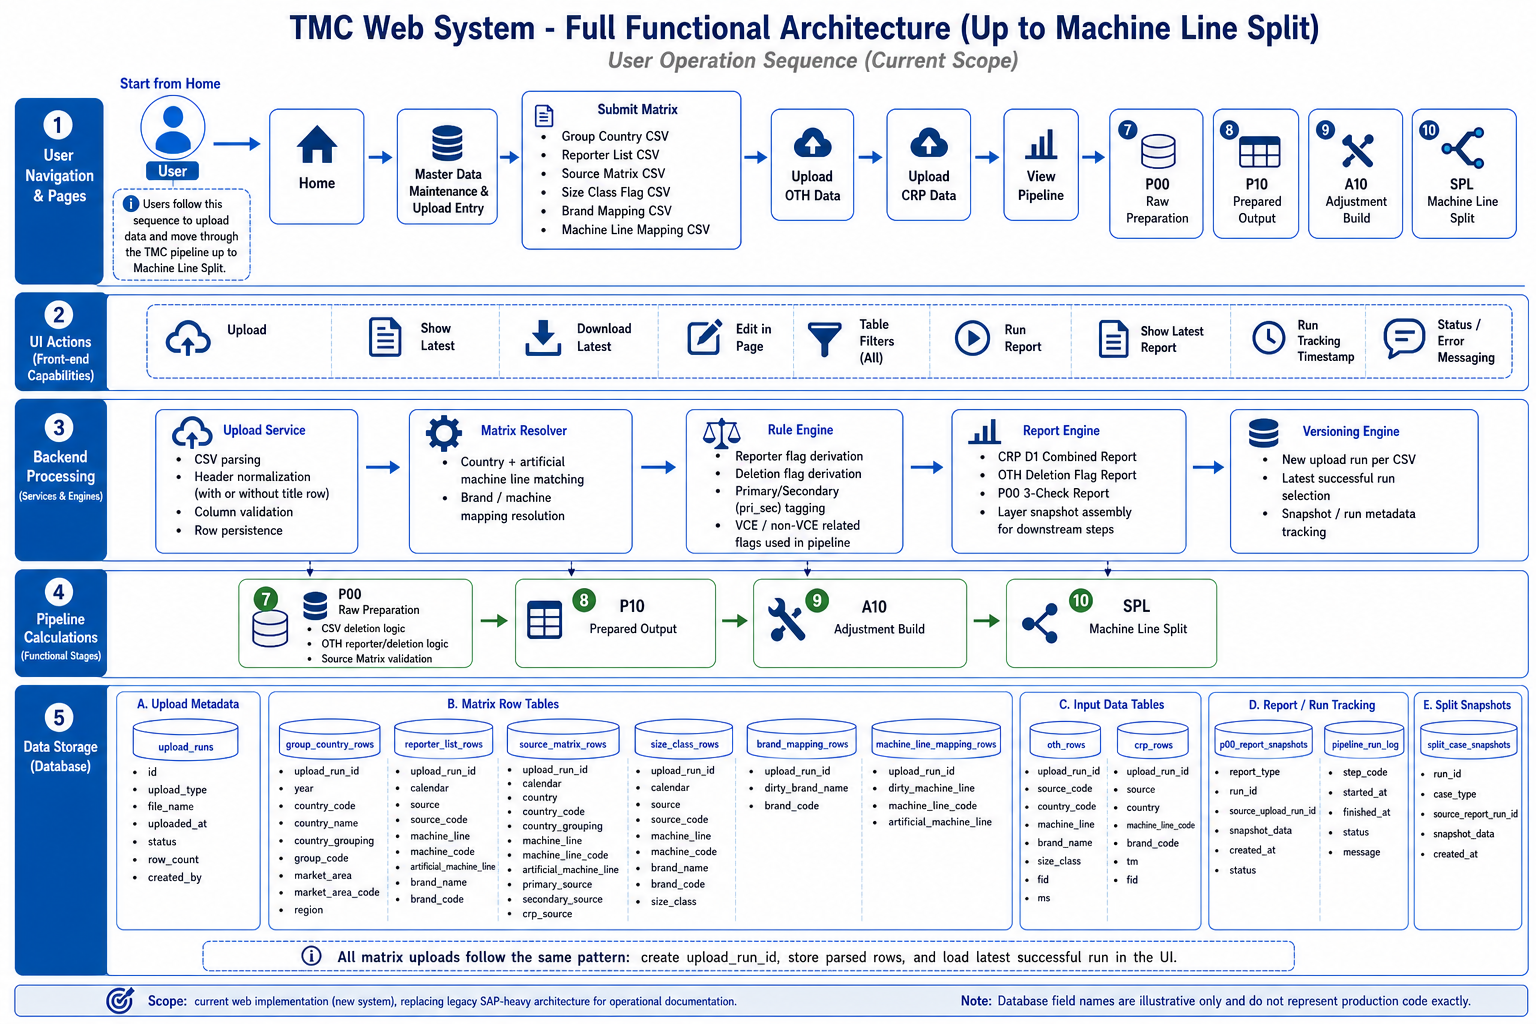
\includegraphics[width=1.0\linewidth]{5.1.png}
%     \caption{ High-level architecture of the web-based TMC artefact}
%     \label{fig:5.1}
% \end{figure}


% The artefact consists of several core elements: (1) support for source data and matrix inputs required in the TMC workflow, (2) backend services that execute workflow logic and organize intermediate and derived outputs, (3) workflow-oriented frontend views for inspecting preparation, adjustment, and split results, and (4) interactive functions such as filtering, summary calculation, and CSV export. Together, these elements form a coherent prototype environment for representing and reviewing selected parts of the TMC workflow in a more transparent and inspectable way.

% In the context of this thesis, the artefact serves as the central design contribution. It demonstrates how parts of a complex enterprise calculation workflow can be transformed into a web-based prototype that improves workflow visibility and user interaction while remaining extensible for future internal use within Volvo CE.



To address the identified gap in transparency, inspectability, and usability in the SAP-based TMC workflow, this thesis develops a web-based artefact for Volvo CE that re-expresses selected parts of the workflow in a browser-accessible environment. The implemented system covers authentication, CSV-based data upload, backend processing, workflow inspection, and review of intermediate and derived outputs for the preparation, adjustment, and machine-line split stages.

The artefact combines a frontend application, backend services, workflow-oriented inspection views, and interactive review functions. Rather than acting only as a reporting interface, it supports a workflow-oriented process in which users can upload data, trigger processing, inspect intermediate results, and review derived outputs within one environment. Together, these elements form a coherent web application for representing and reviewing selected parts of the workflow in a more transparent and inspectable way.


















% \section{Structure and Components of the Artefact}

% \subsection{System Architecture}

% The system architecture of the artefact is shown in Figure 5.1. It illustrates how the prototype is organized into a user interface layer, a backend application layer, and a database layer, together with the flow of uploaded input data, workflow processing, and generated outputs.


% \begin{figure}[H]
%     \centering
%     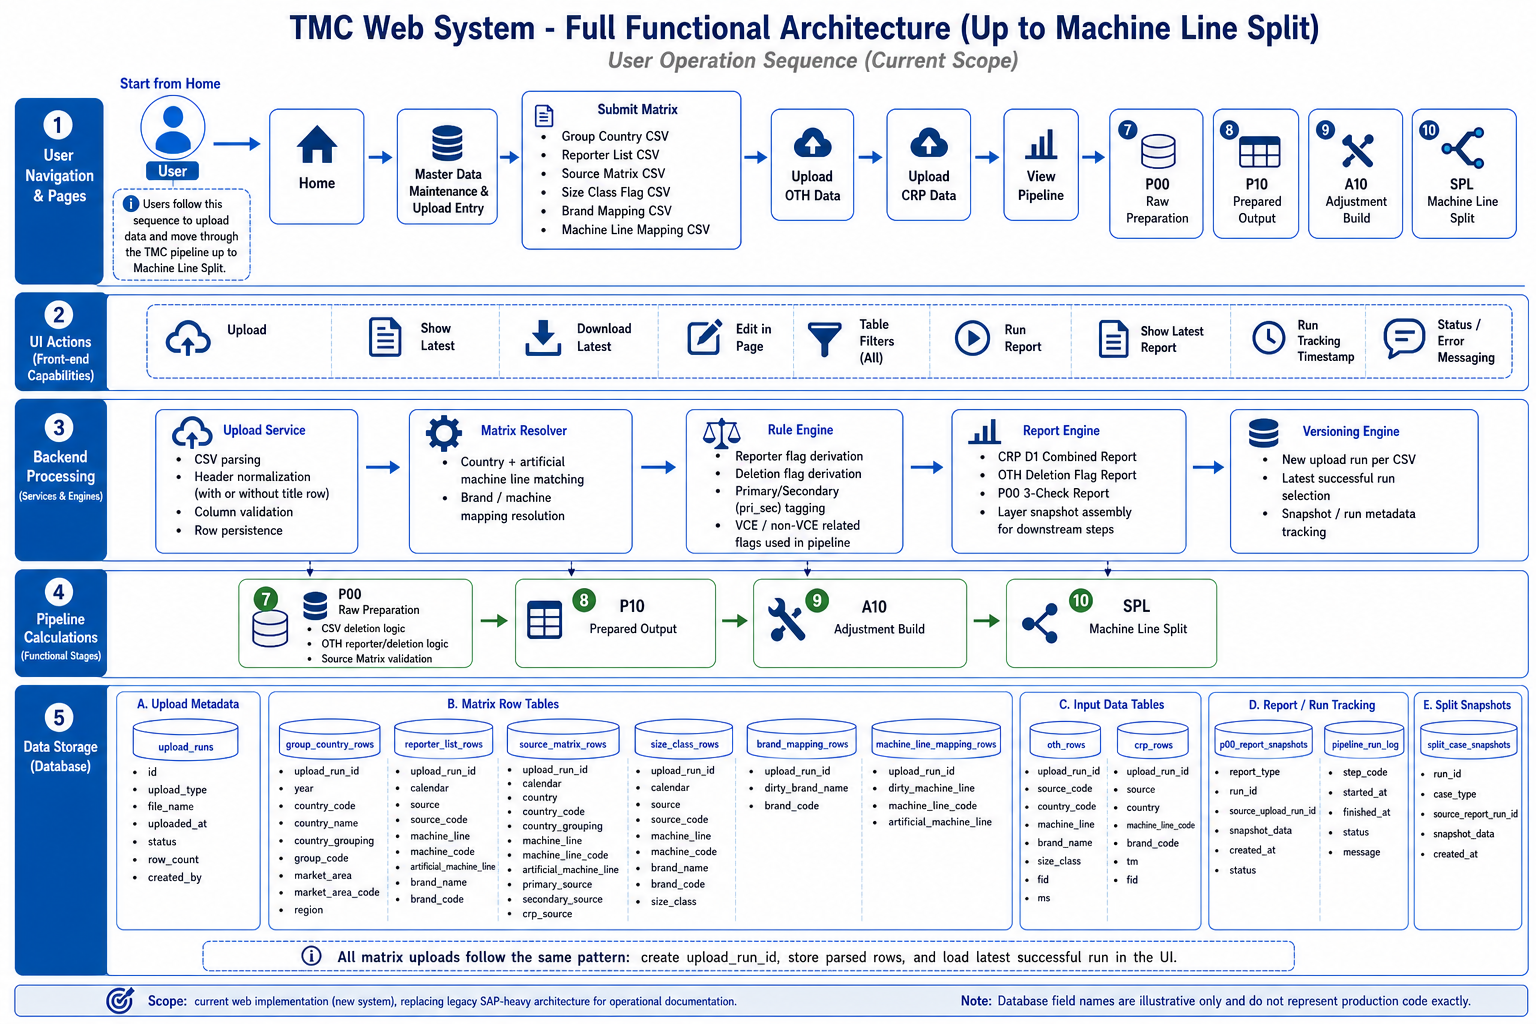
\includegraphics[width=1.0\linewidth]{5.1.png}
%     \caption{ High-level architecture of the web-based TMC artefact}
%     \label{fig:5.1}
% \end{figure}




% On the frontend side, the artefact provides the user interface for navigation, data upload, and inspection of workflow results. This includes views for authentication, homepage-based workflow access, upload of workflow-related CSV files, and layer-based inspection of preparation-, adjustment-, and split-related outputs. The frontend is therefore responsible not only for displaying results, but also for supporting interaction with the workflow in a more transparent and user-oriented way.

% On the backend side, the artefact is implemented through Python-based services that handle file upload, data ingestion, workflow processing, and access to derived outputs. Uploaded files are stored and organized in a structured way, and selected parts of the original SAP-based workflow logic are re-expressed through backend processing supported by SQL-backed storage and querying. This makes it possible to handle workflow-related transformations in a prototype environment that is more inspectable than the original SAP-based representation.

% Between the frontend and backend, the artefact uses API-based communication to transfer uploaded files, request workflow data, and retrieve processed outputs for presentation in the interface. The architecture also includes structured storage for workflow records, mappings, and intermediate outputs, allowing the different workflow stages to be represented in a coherent and modular way.


\section{Overall Design}

\subsection{System Architecture}

The system architecture of the artefact is shown in Figure 5.1. It is organized as a split frontend-backend web application with a persistent data layer, where the frontend provides the user interface, the backend handles authentication and workflow processing, and the database stores uploaded data, session information, and generated outputs. This structure supports browser-based interaction while keeping the implementation modular and easier to maintain.

\begin{figure}[H]
    \centering
    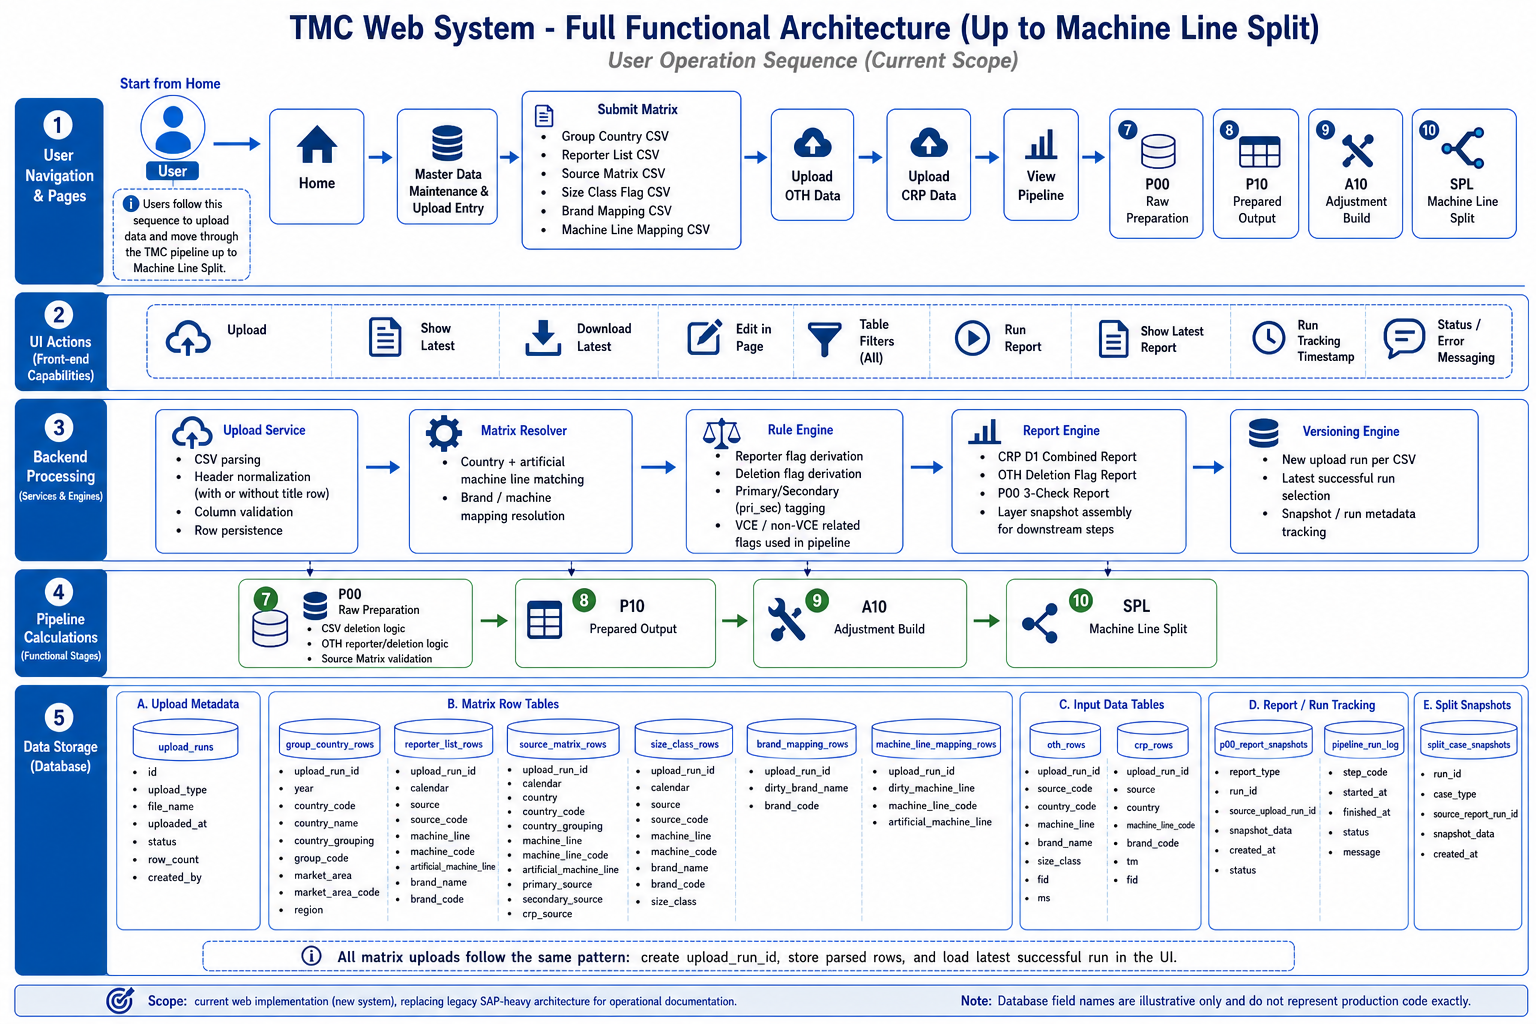
\includegraphics[width=1.0\linewidth]{5.1.png}
    \caption{ High-level architecture of the web-based TMC artefact}
    \label{fig:5.1}
\end{figure}


The frontend is implemented as a single-page application using React and Vite. It uses client-side routing to move between the home page, matrix submission page, upload pages, Pipeline Viewer, and Layer Detail pages. This supports a more interactive review experience.

The backend is implemented with FastAPI and exposes the API endpoints used by the frontend. It also contains the processing logic for the implemented workflow, including file validation, structured storage, and retrieval of intermediate and final outputs.

The data layer is configured through environment variables and supports both SQLite and PostgreSQL. Authentication data is stored separately from the business workflow data, which keeps session management isolated from the calculation data. Communication between the frontend and backend is API-based, so uploaded files, workflow requests, and processed outputs can be exchanged and displayed in structured views such as tables, summaries, and pipeline status cards.




























\subsection{Workflow and Data Flow}

% The execution flow of the artefact follows the staged structure of the implemented TMC workflow. It begins with upload of source data and matrix files and continues through backend cleaning, preparation, adjustment, and split-related processing until the results are exposed in the frontend for inspection.

% The workflow proceeds through the following steps:

% \begin{enumerate}
%     \item \textbf{Upload of source and matrix data.}  
%     Users upload the CSV files required for the workflow through the web interface. In the current prototype, these include source matrix, reporter list, size class, brand mapping, group country, machine line mapping, OTH data, Volvo sales data, and TMA data.

%     \item \textbf{Registration of upload runs.}  
%     Each upload is registered in the \texttt{upload\_runs} table together with metadata such as file name, upload time, status, and row count. This makes it possible to identify the latest successful upload for each data type.

%     \item \textbf{Validation and cleaning in the backend.}  
%     After upload, the files are processed in Python-based backend services. At this stage, the system:
%     \begin{itemize}
%         \item validates the file structure for the selected upload type,
%         \item removes header rows or repeated header-like rows where needed,
%         \item normalizes column names and field values,
%         \item restructures legacy layouts such as the older OTH format,
%         \item standardizes important fields such as size class and size-class mapping.
%     \end{itemize}

%     \item \textbf{Storage in SQL-backed tables.}  
%     The cleaned data is stored in dedicated SQLite tables.
%     \item \textbf{Generation of cleaned intermediate reports.}  
%     Before the main workflow reports are built, the system generates cleaned intermediate outputs:
%     \begin{itemize}
%         \item \texttt{control\_report\_clean\_rows}, which enriches OTH data with mapped country, region, machine line, and brand information,
%         \item \texttt{crp\_tma\_report\_rows}, which aggregates TMA data into a normalized report structure.
%     \end{itemize}

%     \item \textbf{Preparation-stage processing.}  
%     The backend then combines TMA and Volvo sales data into a shared relational structure. At this stage:
%     \begin{itemize}
%         \item TMA data is aggregated into a \texttt{tma\_agg} structure,
%         \item Volvo sales data is aggregated into a \texttt{volvo\_agg} structure,
%         \item country information is resolved from the latest group-country upload,
%         \item artificial machine line is matched from the machine-line mapping upload,
%         \item source matrix logic is used to evaluate country plus artificial-machine-line combinations,
%         \item reporter-list logic is used to assign reporter flags,
%         \item deletion logic is applied to relevant SAL rows.
%     \end{itemize}
%     The main output of this step is the CRP D1 combined preparation report.

%     \item \textbf{P00 and three-check representation.}  
%     The preparation result is then combined with the OTH deletion-flag report to produce the P00 three-check report. This creates one reviewable table containing TMA, SAL, and OTH rows together with matched workflow measures such as TM, VCE FID, and TM Non VCE.

%     \item \textbf{P10 prepared-layer aggregation.}  
%     The preparation output is regrouped into the P10 report. At this stage:
%     \begin{itemize}
%         \item Total Market is calculated from TMA rows,
%         \item VCE is calculated from valid SAL rows with reporter flag \texttt{Y},
%         \item Non-VCE is calculated as \texttt{max(TMA - VCE, 0)}.
%     \end{itemize}

%     \item \textbf{A10 adjustment-stage output.}  
%     The A10 report summarizes SAL and TMA rows into one reviewable result structure for each matched workflow group. It includes detail rows and derived result rows, making the adjustment stage inspectable in the prototype.

%     \item \textbf{Split-related processing.}  
%     The current split-related implementation focuses on excavator split cases. OTH rows are filtered by artificial machine line and size-class conditions, Volvo rows are deducted, and the remaining FID is redistributed using the prepared P10 non-VCE structure as reference. The outputs include both summary rows and detailed split rows.

%     \item \textbf{Frontend inspection and result access.}  
%     The generated outputs are exposed through backend APIs and shown in the frontend as layer-based views, filterable tables, and downloadable results.
% \end{enumerate}

% The final outputs of the artefact therefore include not only uploaded and cleaned datasets, but also staged workflow reports such as the


% The execution flow of the artefact begins with CSV-based upload of the datasets required for the TMC workflow and continues through backend cleaning, preparation, adjustment, and split-related processing until the resulting outputs are made available in the frontend.

% The main execution logic can be summarized as follows:

% \begin{itemize}
%     \item \textbf{CSV upload.}  
%     The workflow starts when users upload the required CSV files through the web interface. In the current prototype, these inputs include source matrix, reporter list, size class input, brand mapping, group country, machine line mapping, OTH data, Volvo sales data, and TMA data.

%     \item \textbf{Validation and cleaning of uploaded data.}  
%     After upload, the backend validates the file structure and performs dataset-specific cleaning. This includes removal of header rows or repeated header-like rows, handling of layout variations, normalization of textual values, and standardization of important fields such as size class. The cleaned CSV content is then transformed into a consistent internal structure.

%     \item \textbf{Generation of cleaned source-level data.}  
%     The cleaned inputs are reorganized into structured source-level outputs. OTH data is combined with country, machine-line, and brand-related mapping data, while TMA data and Volvo sales data are prepared in forms that can be aligned in later workflow stages.

%     \item \textbf{Preparation-stage processing.}  
%     In the preparation stage, the cleaned source datasets are brought into a shared workflow structure. At this stage, country mapping, artificial machine-line mapping, source-related logic, and reporter-related logic are applied in order to generate the first workflow-oriented outputs. The result of preparation is therefore an inspectable structure in which TMA and Volvo sales records can be reviewed together with the relevant workflow flags and aligned dimensions.

%     \item \textbf{Preparation outputs.}  
%     The preparation stage produces:
%     \begin{itemize}
%         \item a preparation-layer output for TMA and Volvo sales related records,
%         \item a cleaned OTH-oriented output with mapped workflow fields,
%         \item a combined review output that brings together TMA, SAL, and OTH-related rows in one inspectable structure.
%     \end{itemize}

%     \item \textbf{Prepared market-view output.}  
%     After preparation, the prototype derives a more compact market-oriented output in which the main workflow measures are summarized. At this stage, the system presents total market, Volvo CE-related values, and non-Volvo CE-related values in a form suitable for review.

%     \item \textbf{Adjustment-stage processing.}  
%     The adjustment stage reorganizes the prepared results into a reviewable adjustment-oriented structure. In the current implementation, this stage makes it possible to inspect both source-detail rows and the derived result rows for the same workflow group.

%     \item \textbf{Split-related processing.}  
%     The split stage redistributes grouped OTH values into more detailed output structures. In the implemented split cases, the starting point is an OTH row whose machine-line category is broader than the intended final output. The prototype therefore uses the prepared market-view result as a reference basis for split.

%     \item \textbf{How split ratios are determined.}  
%     The split ratio is derived from the non-Volvo CE distribution in the prepared output. For a broader grouped value, the system identifies the relevant smaller target buckets and calculates each ratio as the reference value of that bucket divided by the sum of the relevant reference values. The original OTH value is then multiplied by these ratios in order to obtain the split results. When detailed reference data is not available at country level, the current implementation applies a fallback logic through broader aggregation levels.

%     \item \textbf{Final outputs.}  
%     The final outputs are not limited to one single result table. Instead, the artefact produces a sequence of staged outputs, including cleaned source-level outputs, preparation-layer outputs, combined review outputs, prepared market-view results, adjustment-stage results, and split-related results. These are displayed in the frontend as workflow-layer views, filterable tables, summary values, and downloadable results.
% \end{itemize}


The execution flow of the artefact begins with browser-based upload of the datasets required for the TMC workflow and continues through backend validation, cleaning, persistence, processing, and frontend inspection. Each upload is registered together with metadata such as file name, upload time, status, and row count. This makes it possible to identify the latest valid input for each data type and to trace how the workflow was executed.


\begin{figure}[H]
    \centering
    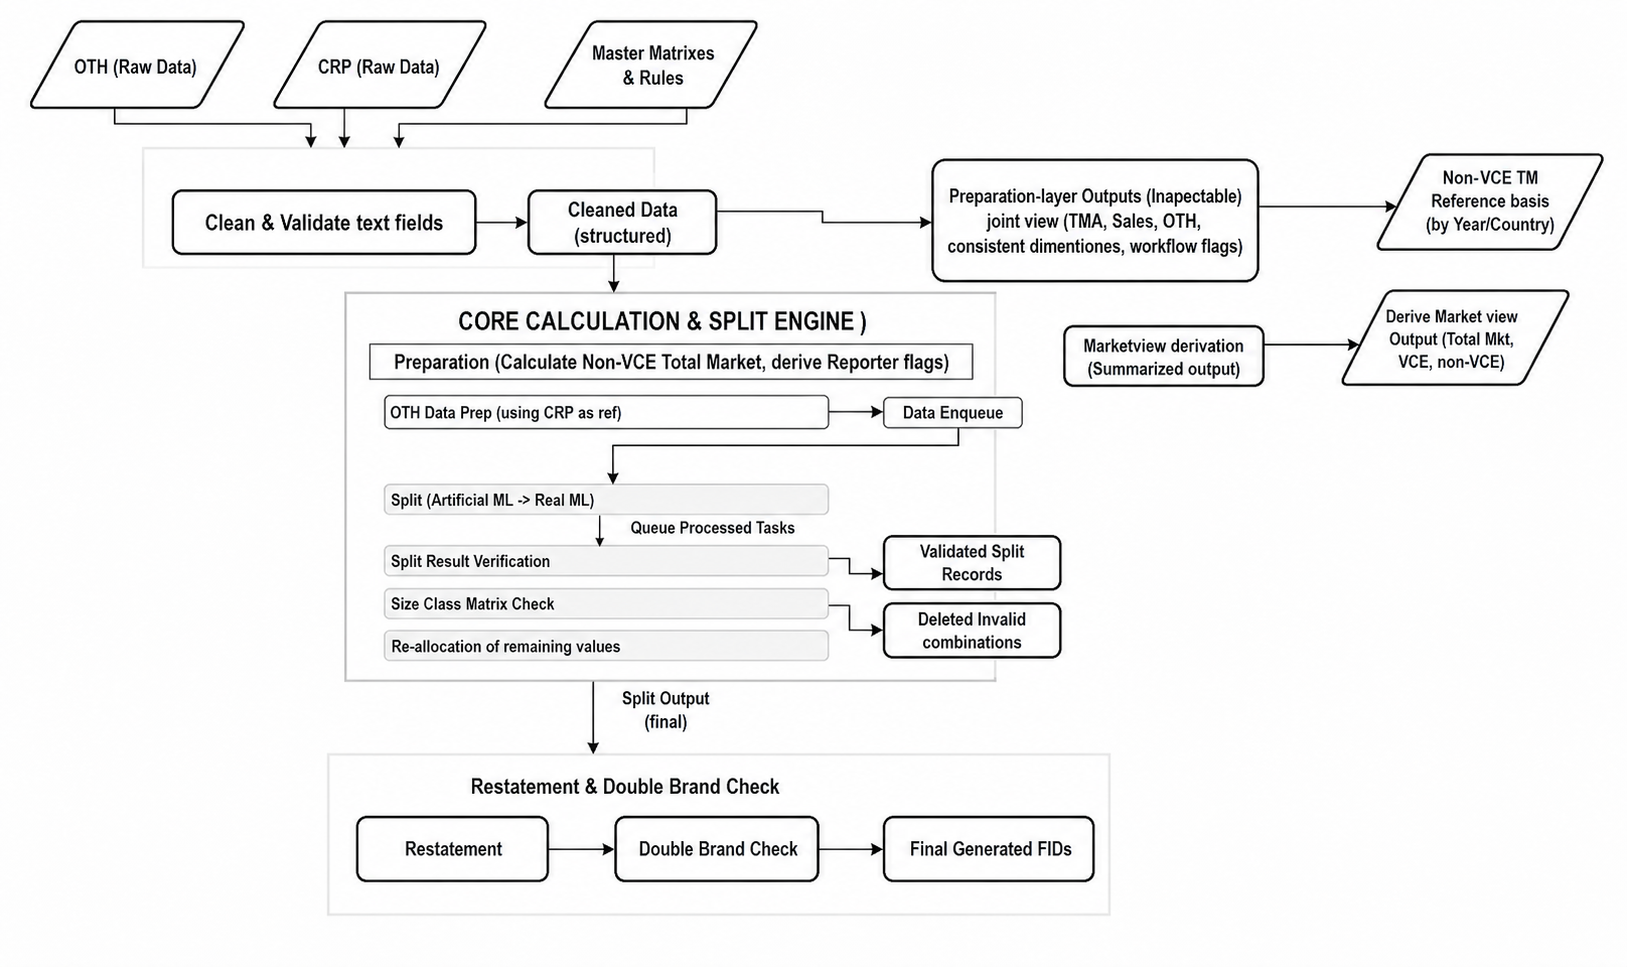
\includegraphics[width=1.2\linewidth]{5.2.1.png}
    \caption{Data Flow and Processing Stages of the TMC Artefact}
    \label{fig:5.2}
\end{figure}







\begin{itemize}
    \item \textbf{CSV upload and validation.}  
    The workflow starts with users uploading the required source and matrix files through the web interface. The backend validates file structure and performs dataset-specific cleaning, such as removing header rows, normalising textual values, and standardising key fields.

    \item \textbf{Source-level data preparation.}  
    The cleaned inputs are transformed into structured source-level data. OTH data is combined with mapping tables, while TMA and Volvo sales data are prepared for alignment in subsequent stages.

    \item \textbf{Preparation stage.}  
    In this stage, datasets are aligned within a shared workflow structure. Country mapping, artificial machine-line mapping, source logic, and reporter determination are applied to produce inspectable preparation-layer outputs that bring TMA, Volvo sales, and OTH data into consistent dimensions.

    \item \textbf{Market-view derivation.}  
    A summarized market-oriented output is derived from the preparation results, presenting total market, Volvo CE values, and non-Volvo CE values in a compact and reviewable form.

    \item \textbf{Adjustment stage.}  
    The adjustment stage reorganizes the prepared data into a structure that allows inspection of both source-level records and derived results within the same workflow context.

    \item \textbf{Split processing.}  
    The split stage redistributes grouped OTH values into more detailed categories. The prepared market-view output is used as a reference basis, and split ratios are derived from the non-Volvo CE distribution. When detailed reference data is unavailable at country level, fallback logic based on higher-level aggregation is applied.

    \item \textbf{Final outputs and presentation.}  
    The artefact produces multiple staged outputs, including cleaned data, preparation-layer outputs, adjustment results, and split results. These are presented in the frontend as workflow views, filterable tables, summary metrics, and downloadable files.
\end{itemize}




% \section{Functions and Behaviour of the Core Component}


\section{Detail Design}

% \subsection{CSV Upload and Input Handling}



% A central function of the artefact is to support structured upload of workflow-related CSV files through the web interface. The upload and input-handling component provides the data foundation for the subsequent workflow stages.

% The uploaded inputs in the current prototype can be grouped into the following categories:

% \begin{itemize}
%     \item market-related source data CSV,
%     \item sales-related source data CSV,
%     \item reference market data CSV,
%     \item source-definition matrices CSV,
%     \item reporter and mapping inputs CSV,
%     \item country and grouping definitions CSV,
%     \item machine-line and size-class-related mapping data CSV.
% \end{itemize}

% These inputs have different roles in the workflow. Some provide the market and sales values that are processed in later stages, while others define how the source records should be aligned, grouped, interpreted, and redistributed.

% After upload, each file is registered together with metadata such as upload type, file name, upload time, status, and row count. This allows the prototype to identify the latest successful version of each required input and use it as the basis for later workflow execution.

% The uploaded data is finally reflected in the artefact through:

% \begin{itemize}
%     \item upload views showing whether the required input categories are available,
%     \item result views showing upload status and basic upload information,
%     \item workflow-layer views in which the uploaded inputs are transformed into preparation-, adjustment-, and split-related outputs.
% \end{itemize}



\subsection{CSV Upload and Input Handling}

A central function of the artefact is to support structured upload of workflow-related CSV files through the web interface. This component provides the data foundation for the later workflow stages and is accessed through dedicated frontend entry points such as the matrix submission page, upload pages, the Pipeline Viewer, and Layer Detail views.

The uploaded inputs in the current prototype can be grouped into market data, sales data, reference market data, source-definition matrices, and mapping-related inputs such as reporter, country, machine-line, and size-class definitions.

After upload, each file is registered with metadata such as upload type, file name, upload time, status, and row count. This allows the prototype to identify the latest successful version of each required input and use it as the basis for later workflow execution and inspection.

The uploaded data is then reflected in upload views, result views, and workflow-stage views.

























 % \subsection{Data Cleaning and Workflow Preparation}



% The preparation stage is the first workflow-oriented processing stage in the artefact. Its purpose is to transform the uploaded source data and mapping input into structured results that can be reviewed before later adjustment and split-related processing.

% The main functions of this stage are:

% \begin{itemize}
%     \item aligning uploaded source records with the relevant workflow definitions, including country-related grouping logic, machine-line-related mapping, source definitions, and reporter-related input,
%     \item assigning workflow control fields such as deletion flag, reporter flag, and source-related preparation indicators,
%     \item reorganizing source records from different origins into a shared workflow structure,
%     \item generating preparation-level outputs that can be inspected before later workflow stages are applied.
% \end{itemize}

% For OTH-related records, the preparation stage includes the following processing:

% \begin{itemize}
%     \item the uploaded rows are first aligned with country, machine-line, and brand-related mappings,
%     \item rows that belong to the same mapped workflow combination are then aggregated and their values are summed into preparation-ready results,
%     \item the resulting structured rows are used as the OTH-oriented preparation output for later review and downstream workflow processing.
% \end{itemize}

% For TMA- and sales-related records, the preparation stage produces a comparable workflow representation in which different source categories can be reviewed together. This makes it possible to inspect the data in a shared structure instead of as isolated uploaded files.

% The outputs of this stage are reflected in the artefact through preparation-layer views and combined review-oriented results. These outputs provide the first inspectable representation of how uploaded input data is transformed inside the prototype and serve as the basis for the later market-view, adjustment, and split-related stages.



\subsection{Preparation Stage}

% The preparation stage is the first workflow-oriented processing stage in the artefact. Its purpose is to transform uploaded source data and mapping input into structured results that can be reviewed before later adjustment and split and resplit processing.

% The preparation stage in the current prototype consists of the following main steps. Together, these steps make early workflow transformations visible before later market-view, adjustment, and split-related processing is applied:

% \begin{itemize}
%     \item \textbf{OTH-oriented preparation.}  
%     Uploaded OTH rows are first aligned with country-related grouping input, machine-line mapping, brand mapping, source matrix, and reporter-related input. After this alignment, the artefact assigns preparation control fields such as deletion flag, Pri/Sec, and reporter flag. Rows that belong to the same mapped workflow combination are then aggregated and their values are summed into a structured OTH-oriented preparation output.

%     \item \textbf{CRP/TMA/SAL-oriented preparation.}  
%     TMA and sales-related records are reorganized into a shared workflow structure. At this stage, the artefact applies country mapping, artificial machine-line mapping, source-matrix-related logic, and reporter-related matching in order to produce preparation-level records. The resulting output makes it possible to review TMA- and sales-related source categories together within one comparable structure.

%     \item \textbf{Assignment of workflow control logic.}  
%     A central function of the preparation stage is to make workflow logic explicit in the artefact. In the current implementation, this includes preparation-related fields such as deletion flag and reporter flag, together with source-related classification logic used for later workflow interpretation.

%     \item \textbf{Combined preparation review output.}  
%     After the OTH-oriented and CRP/TMA/SAL-oriented preparation outputs have been generated, the artefact produces a combined review-oriented result in which TMA, SAL, and OTH-related rows can be inspected within a shared workflow view. This gives the user an early overview of how the uploaded input data has been transformed before later stages are applied.
% \end{itemize}

% The outputs of this stage are reflected in the artefact through preparation-layer views and review-oriented tables. These outputs provide the basis for the later market-view, adjustment, and split-related stages, while also allowing users to inspect the preparation logic in a more explicit and transparent way than in the original SAP-based environment.




The preparation stage is the first workflow-oriented processing stage in the artefact. Its purpose is to transform uploaded source data and mapping input into structured results that can be reviewed before later adjustment and split and resplit processing.

The preparation stage in the current prototype consists of the following main steps. Together, these steps make early workflow transformations visible before later market-view, adjustment, and split-related processing is applied:

\begin{itemize}
    \item \textbf{OTH-oriented preparation.}  
    Uploaded OTH rows are aligned with country-related grouping input, machine-line mapping, brand mapping, source matrix, and reporter-related input. During this step, backend logic assigns preparation control fields such as deletion flag, Pri/Sec, and reporter flag. Rows that belong to the same mapped workflow combination are then aggregated into a structured OTH-oriented preparation output.

    \item \textbf{CRP/TMA/SAL-oriented preparation.}  
    TMA and sales-related records are reorganised into a shared workflow structure through SQL-based grouping, joins, and aggregation. Country mapping, artificial machine-line mapping, source-matrix logic, and reporter-related matching are applied to produce preparation-level records that can be reviewed together.

    \item \textbf{Combined preparation review output.}  
    After the OTH-oriented and CRP/TMA/SAL-oriented preparation outputs have been generated, the artefact exposes them through backend APIs and renders them in workflow views. This produces a combined review-oriented result in which TMA, SAL, and OTH-related rows can be inspected before later stages are applied.
\end{itemize}






% \subsection{Adjustment and Split Stage}



% After the preparation stage, the artefact represents the subsequent workflow through adjustment-oriented and split-related outputs. This component is implemented through React-based frontend views, FastAPI endpoints, and SQL-backed backend processing.

% The main functions of this component are:

% \begin{itemize}
%     \item reorganizing prepared TMA- and SAL-related rows into adjustment-oriented result structures,
%     \item generating source-detail rows together with derived result rows for the same workflow group,
%     \item applying split-related logic to selected grouped OTH values,
%     \item exposing both adjustment and split-related outputs through reviewable frontend views.
% \end{itemize}

% In the adjustment stage, the backend groups the prepared workflow data along shared workflow dimensions and generates an output that includes SAL detail rows, TMA detail rows, and one derived result row for each matched workflow group. This makes it possible to inspect how the adjusted result is formed from the prepared records rather than only showing a final aggregated value.

% In the split-related stage, the backend combines prepared OTH-oriented data with the prepared market-view output. Grouped OTH values are filtered, Volvo-related values are deducted, and split ratios are derived from the prepared non-Volvo CE distribution in order to redistribute the remaining value into more detailed result structures.

% The resulting outputs are returned through backend APIs and rendered in the frontend as workflow-layer views and filterable tables. In this way, the artefact makes the later workflow stages both executable in the backend and inspectable in the frontend.



\subsection{Adjustment and Split Stage}

After preparation, the artefact continues with adjustment-oriented and split and resplit processing.

The main functions of this component are:
\begin{itemize}
    \item regrouping prepared TMA and SAL rows into adjustment outputs,
    \item splitting grouped OTH values into more detailed machine-line and size-class buckets,
    \item calculating split ratios from the prepared non-Volvo CE distribution,
    \item supporting resplit and manual correction for selected split cases.
\end{itemize}

The adjustment stage produces an intermediate review result organised around shared workflow keys such as country and machine line. In this output, TMA and SAL rows for the same country and machine line are brought together, making it easier to inspect how the adjusted result is formed.

The split stage is needed because uploaded OTH data is not always available at the granularity required by the workflow. In this stage, aggregated OTH values are redistributed into smaller target buckets using split ratios derived from a non-Volvo CE reference distribution. The prepared market-view output provides the reference basis, with Volvo CE sales excluded before proportional ratios are calculated.

For selected cases, the prototype also supports a resplit step that recalculates the split using source-matrix and size-class mappings before the resulting rows are saved. This step is needed because some brands may be active in a country and machine line, but not in all size classes within that market. In such cases, the prototype uses the source matrix and size-class matrix to determine valid size classes and reallocate values from invalid brand--machine-line--size-class combinations to valid target buckets.

The resulting outputs are returned through backend APIs and rendered in the frontend as workflow-stage views and filterable tables. In this way, the implemented adjustment and split and resplit stages are both executable in the backend and inspectable in the frontend.















% \subsection{Visualization and Interaction}

% The visualization and interaction layer presents workflow results through the React-based frontend. In the current prototype, backend-generated outputs are shown through summary-oriented dashboard views, chart-based representations, and filterable tables.

% This layer supports both overview and detailed inspection. Dashboard elements and charts provide a compact view of selected workflow values, while table-based views allow users to inspect the underlying rows in a way that is closer to spreadsheet-based work. Users can filter the displayed data, review grouped values, and inspect summary calculations directly in the interface. In particular, after filtering, the interface can display the summed values of the filtered result set at the top of the table view, which supports quick validation and comparison.

% The component also supports CSV export of selected results. This allows workflow outputs to be downloaded for further review and analysis outside the artefact. In this way, the visualization layer combines dashboard-style presentation, spreadsheet-like inspection, dynamic summary feedback, and export functionality in one web-based environment.


\subsection{Visualization and Interaction}

The visualization and interaction layer presents uploaded data and workflow results through the React-based frontend. In the current prototype, backend-generated outputs and uploaded inputs are shown through workflow-specific views such as the Pipeline Viewer, Layer Detail pages, upload result pages, and table-based inspection views.

This layer supports both overview and detailed inspection. The Pipeline Viewer provides a compact view of the overall workflow status, while the Layer Detail pages allow users to inspect the underlying rows in a way that is closer to spreadsheet-based work. Users can filter the displayed data, review grouped values, and inspect summary calculations directly in the interface. In addition, uploaded data can be edited directly on the page and saved for later workflow steps, which allows small corrections to be made without returning to the original CSV files.

The component also supports CSV export of selected results. This allows workflow outputs to be downloaded for further review and analysis outside the artefact. In this way, the visualization and interaction layer combines workflow overview, row-level inspection, editable uploaded data, dynamic summary feedback, and export functionality in one web-based environment.








% \section{Development Process}



% % The prototype was developed incrementally as a full-stack web application. Rather than implementing the final workflow output directly, development first focused on the technical infrastructure required for authenticated access, page-based navigation, CSV upload, structured storage, and staged report generation. This provided the basis for the later implementation of workflow-specific logic and frontend inspection.

% % The system was implemented with a React- and TypeScript-based frontend and a Python/FastAPI-based backend. The frontend was built with Vite and React Router, which enabled the prototype to be organized into dedicated pages for authentication, upload, workflow navigation, and layer-based inspection. An authentication context was introduced in React to manage login state and protected routes, while a dedicated API client layer connected frontend pages to backend endpoints in a consistent way.

% % \begin{figure}[h]
% %     \centering
% %     % Insert grouped frontend screenshots, e.g. auth page, upload page, layer detail page, filtered table view
% %     \caption{Selected frontend views developed during the implementation of the prototype}
% %     \label{fig:development_frontend_views}
% % \end{figure}

% % On the backend side, FastAPI was used to implement the application service layer. At startup, the backend initializes both the workflow database and the authentication database. Separate routers were implemented for authentication and workflow-related upload/report functionality. The authentication part handles registration, login, session creation, and protected API access, while the workflow router exposes upload, report, and result retrieval endpoints for the frontend.

% % The next major implementation step was CSV upload and relational storage. Uploaded files are submitted from the React upload pages to the FastAPI upload endpoint together with their dataset type. In the backend, dataset-specific Python handlers process each upload according to its role in the workflow. At this stage, \texttt{pandas} is used to read heterogeneous CSV files, remove header rows or repeated header-like rows, handle layout differences, normalize field names and values, and transform the content into a consistent internal structure. The cleaned rows are then stored in SQLite tables, while upload metadata such as file type, file name, upload time, row count, and processing status is stored separately in an upload tracking table.

% % After the upload layer had been completed, development focused on report generation. The first implemented report endpoints produced cleaned source-level outputs for uploaded OTH and TMA data. These reports were generated from the latest successful uploads and were used to verify that source datasets had been parsed and structured correctly before the workflow stages themselves were implemented.

% % \begin{figure}[h]
% %     \centering
% %     % Insert figure or screenshot showing upload-to-preparation processing
% %     \caption{Implementation of CSV upload, cleaning, and preparation-stage report generation}
% %     \label{fig:development_preparation_reports}
% % \end{figure}

% % The preparation stage was implemented next as the first workflow-oriented report layer. Technically, this stage combines Python-based backend orchestration with SQL-based joins, filtering, and aggregation over the stored relational tables. Uploaded source records are aligned with country grouping, machine-line mapping, source matrix logic, and reporter-related input. Workflow control fields such as deletion flag, reporter flag, and source-related classification indicators are generated explicitly in the backend output. For OTH-related records, mapped rows are aggregated into preparation-ready results, while TMA- and sales-related records are reorganized into a shared workflow structure that can later be inspected together.

% % After preparation had been established, the backend was extended with prepared and adjustment-oriented result generation. SQL-based grouped queries were used to regroup preparation results into more compact and reviewable report structures. A key implementation decision at this stage was that the API should not return only one final value table. Instead, the adjustment-oriented output was designed to include both source-detail rows and derived result rows for the same workflow group, so that the frontend could expose how the resulting values are formed.

% % The next implementation step was split-related processing. In the current prototype, this stage combines prepared OTH-oriented outputs with prepared market-view outputs. Python-based backend logic coordinates the execution flow, while SQL-derived grouped reference values are used to determine redistribution ratios. The resulting output includes summary rows, detailed split rows, and supporting reference information, allowing the split logic to be inspected in the frontend rather than remaining hidden as a backend-only calculation.

% % \begin{figure}[h]
% %     \centering
% %     % Insert screenshot showing adjustment or split-related result view
% %     \caption{Implementation of adjustment- and split-related workflow views}
% %     \label{fig:development_adjustment_split_views}
% % \end{figure}

% % Frontend development progressed together with these backend reports. Once the report endpoints were available, the layer detail page was extended to request report data through the API client layer and render the returned JSON results in workflow-specific views. A reusable filterable table component was implemented so that different layers could share the same table logic. This component supports column-based filtering, row counting, and dynamic recalculation of numeric sums for the filtered result set. In addition, summary cards, chart-based representations, and CSV export functionality were added so that users can move between high-level overview and row-level inspection within the same interface.



% The prototype was developed incrementally as a full-stack web application. Instead of implementing the final workflow output directly, development first established the technical infrastructure required for authentication, page navigation, CSV upload, structured storage, and staged report generation. This provided the foundation for later workflow-specific logic and frontend inspection.

% The system consists of a React- and TypeScript-based frontend and a Python/FastAPI-based backend. The frontend, built with Vite and React Router, is organized into pages for authentication, upload, workflow navigation, and layer-based inspection. An authentication context manages login state and protected routes, while an API client layer enables consistent communication with backend endpoints.

% \begin{figure}[H]
%     \centering
%     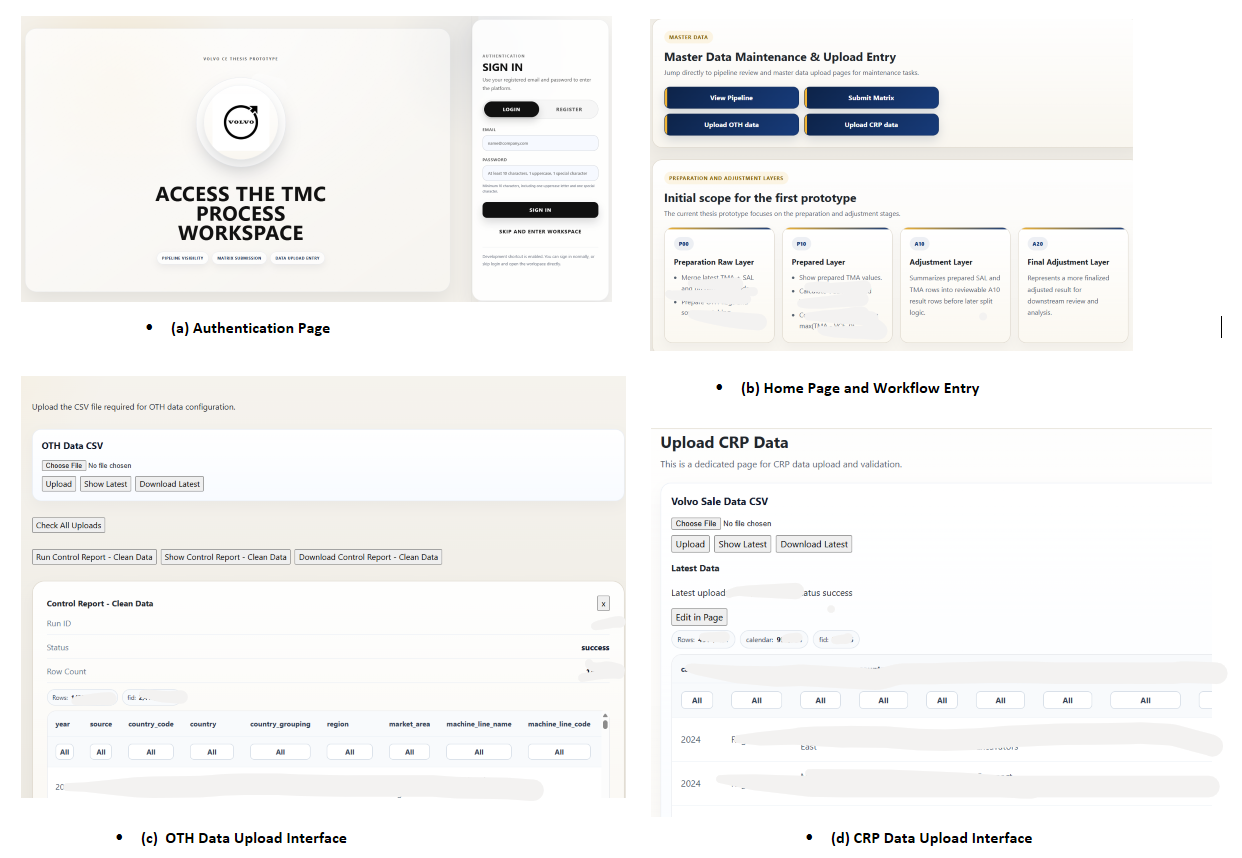
\includegraphics[width=1.0\linewidth]{5.3.png}
%     \caption{Selected frontend views developed during the implementation of the prototype}
%     \label{fig:5.3}
% \end{figure}






% On the backend, FastAPI implements the service layer, with SQLite used for relational storage. At startup, the system initializes workflow and authentication databases, and defines separate routers for authentication and workflow-related functionality. These include endpoints for upload, report generation, and result retrieval.

% The next step focused on CSV upload and data storage. Files are submitted from the frontend together with dataset type information and processed by dataset-specific Python handlers. Using \texttt{pandas}, heterogeneous CSV files are parsed, cleaned, and normalized into a consistent structure. The processed rows are stored in SQLite tables, while upload metadata is tracked separately.

% Once the upload layer was established, development moved to report generation. Initial endpoints produced cleaned source-level outputs for OTH and TMA data, enabling validation of parsing and data alignment.

% \begin{figure}[H]
%     \centering
%     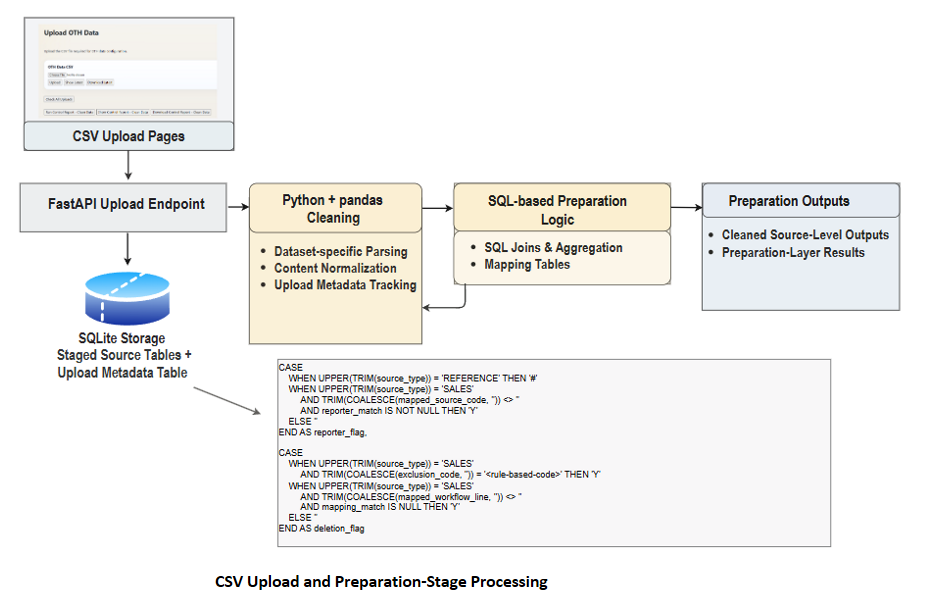
\includegraphics[width=1.0\linewidth]{5.4.png}
%     \caption{Implementation of CSV Upload and Preparation-Stage Processing}
%     \label{fig:5.4}
% \end{figure}



% \begin{figure}[H]
%     \centering
%     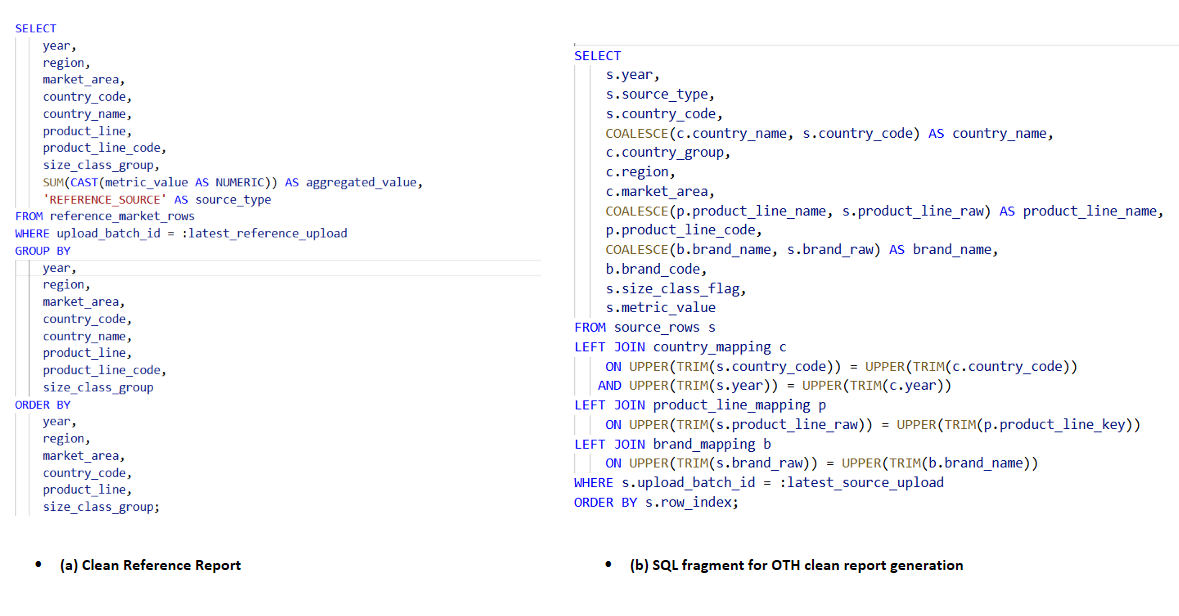
\includegraphics[width=1.0\linewidth]{5.4.1.png}
%     \caption{ Simplified SQL Fragments for CRP/TMA and OTH Clean Report Generation}
%     \label{fig:5.4.1}
% \end{figure}





% The preparation stage was then implemented using SQL-based joins, filtering, and aggregation over stored tables. Source records are aligned with mapping data and enriched with workflow control fields such as deletion and reporter flags. The resulting outputs provide a consistent structure for joint inspection of TMA, sales, and OTH data.

% Subsequently, adjustment and prepared result layers were introduced through grouped SQL queries. A key design decision was to return both source-detail rows and derived results within the same output, allowing the frontend to expose how final values are constructed.

% The split stage was implemented by combining prepared OTH data with market-view outputs. Backend logic coordinates the execution, while SQL-derived reference values are used to calculate redistribution ratios. The resulting outputs include summary rows, detailed split results, and supporting reference values, enabling the split logic to be inspected rather than hidden.



% \begin{figure}[H]
%     \centering
%     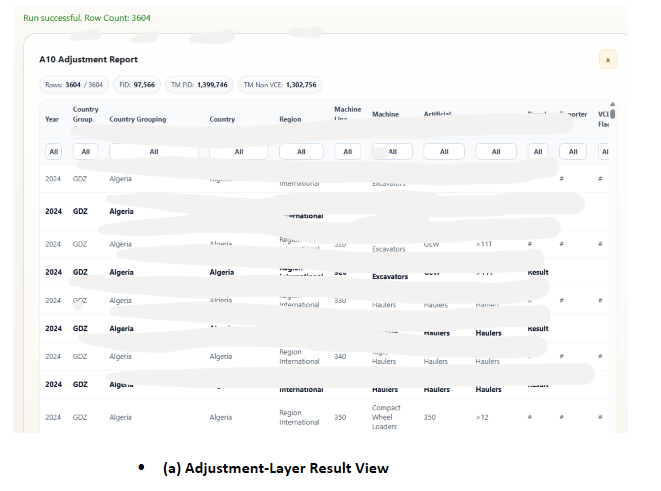
\includegraphics[width=0.9\linewidth]{5.6.1.png}
%     % \caption{Implementation of adjustment- and split-related workflow views}
%     \label{fig:5.6.1}
% \end{figure}





% \begin{figure}[H]
%     \centering
%     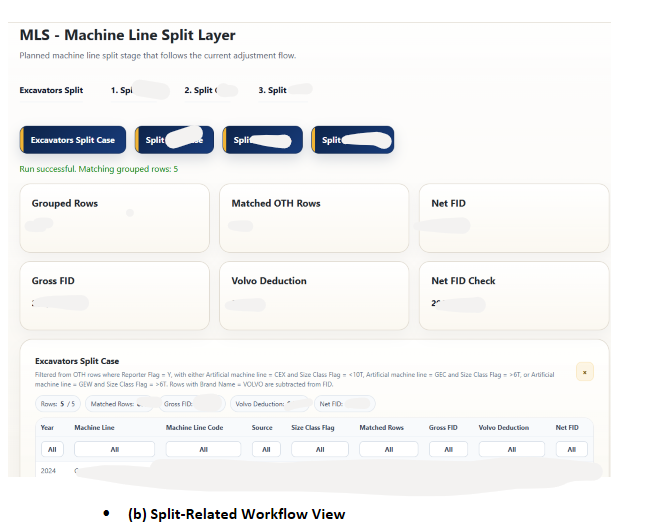
\includegraphics[width=0.9\linewidth]{5.6.2.png}
%     \caption{Implementation of adjustment- and split-related workflow views}
%     \label{fig:5.6.2}
% \end{figure}


% \begin{figure}
%     \centering
%     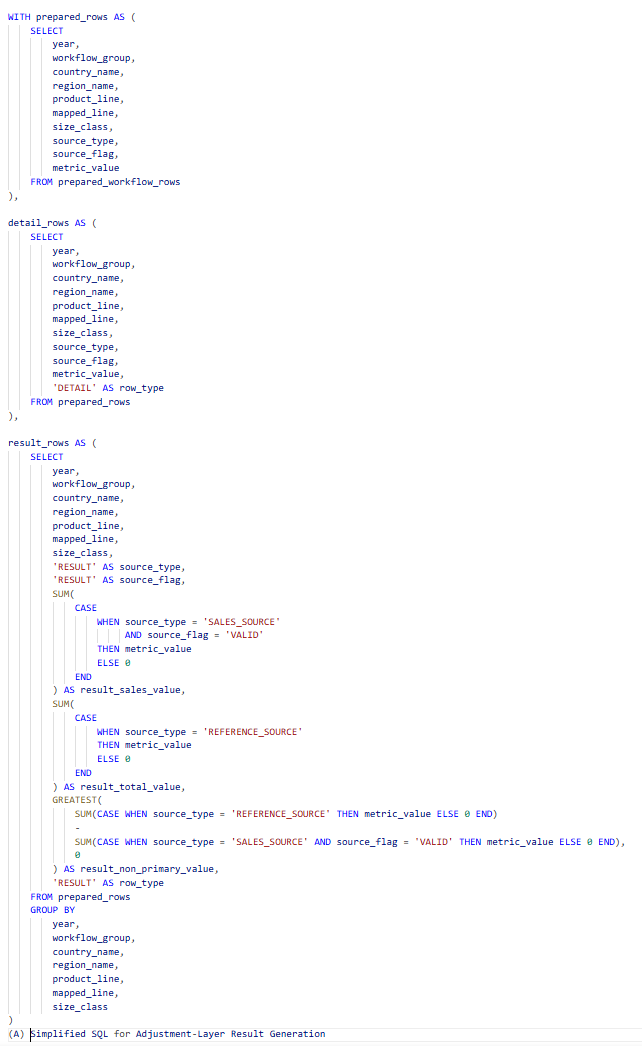
\includegraphics[width=1.1\linewidth]{5.6.3.png}
%     % \caption{Enter Caption}
%     \label{fig:placeholder}
% \end{figure}



% \begin{figure}
%     \centering
%     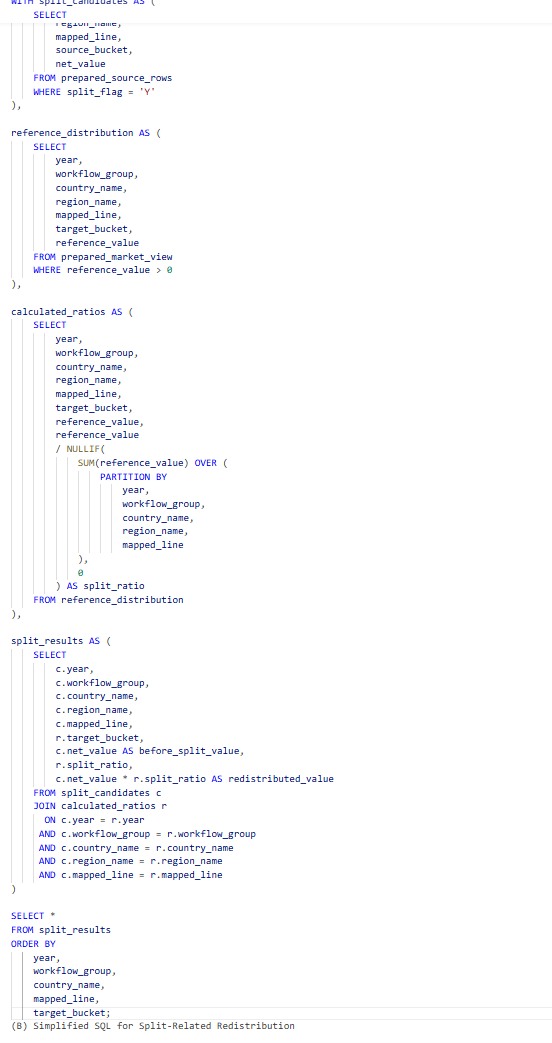
\includegraphics[width=0.85\linewidth]{5.6.4.png}
%     \caption{SQL Fragments for Adjustment- and Split-Related Processing}
%     \label{fig:placeholder}
% \end{figure}




% Frontend development progressed alongside backend reports. Report endpoints return structured JSON data, which is rendered in workflow-specific views. A reusable filterable table component supports column-based filtering and dynamic aggregation, while summary cards, charts, and CSV export provide both detailed and high-level inspection.


% \section{Implementation}

% The prototype was developed incrementally as a full-stack web application. Instead of implementing the final workflow output directly, development first established the technical infrastructure required for authentication, page navigation, CSV upload, structured storage, and staged report generation. This provided the foundation for later workflow-specific logic and frontend inspection.

% The system consists of a React- and TypeScript-based frontend and a Python/FastAPI-based backend. The frontend, built with Vite and React Router, is organized into pages for authentication, matrix submission, upload, workflow navigation, and layer-based inspection. An authentication context manages login state and protected routes, while an API client layer enables consistent communication with backend endpoints.

% \begin{figure}[H]
%     \centering
%     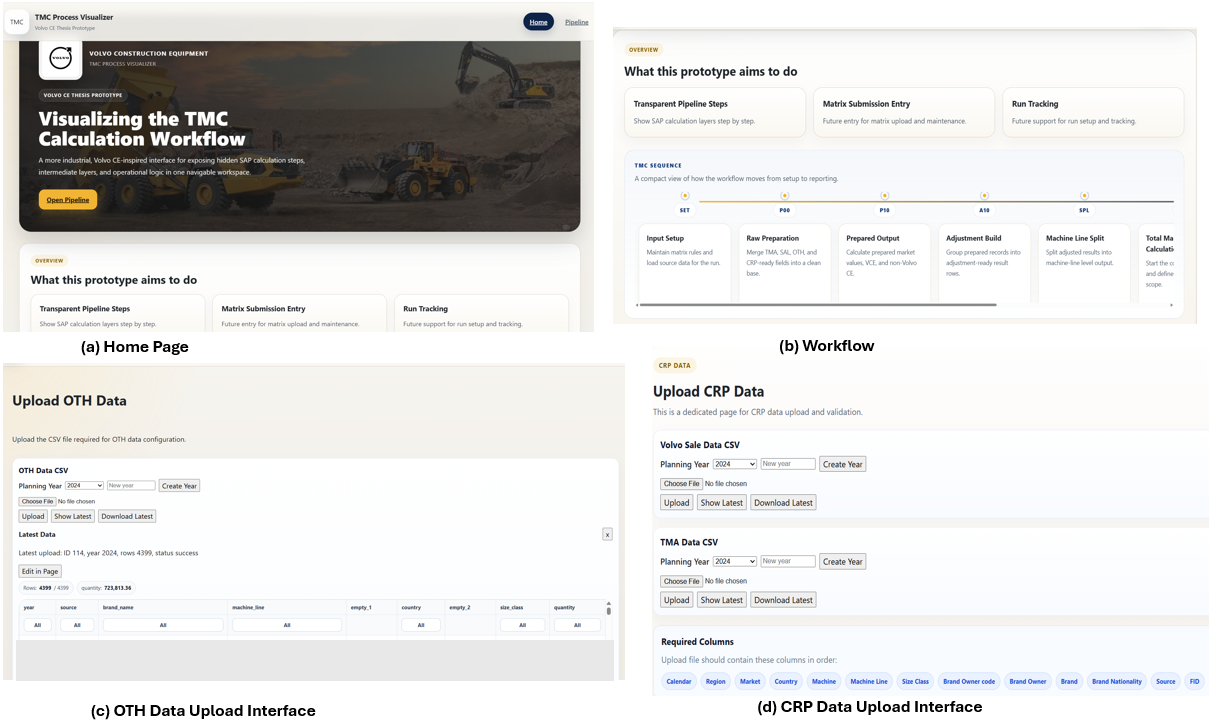
\includegraphics[width=1.1\linewidth]{5.3.1.png}
%     \caption{Selected frontend views developed during the implementation of the prototype}
%     \label{fig:5.3}
% \end{figure}

% On the backend, FastAPI implements the service layer, with a configurable relational data layer that supports SQLite and can be switched to PostgreSQL through environment-based configuration. At startup, the system initializes the workflow and authentication databases and defines separate routers for authentication and workflow-related functionality. These include endpoints for upload, report generation, and result retrieval.

% The next step focused on CSV upload and data storage. Files are submitted from the frontend together with dataset type information and processed by dataset-specific Python handlers. Using \texttt{pandas}, heterogeneous CSV files are parsed, cleaned, and normalized into a consistent structure. The processed rows are stored in the database, while upload metadata is tracked separately so that the latest successful input for each dataset can be reused in later processing steps.

% Once the upload layer was established, development moved to report generation. Initial endpoints produced cleaned source-level outputs for OTH and TMA data, enabling validation of parsing and data alignment.

% \begin{figure}[H]
%     \centering
%     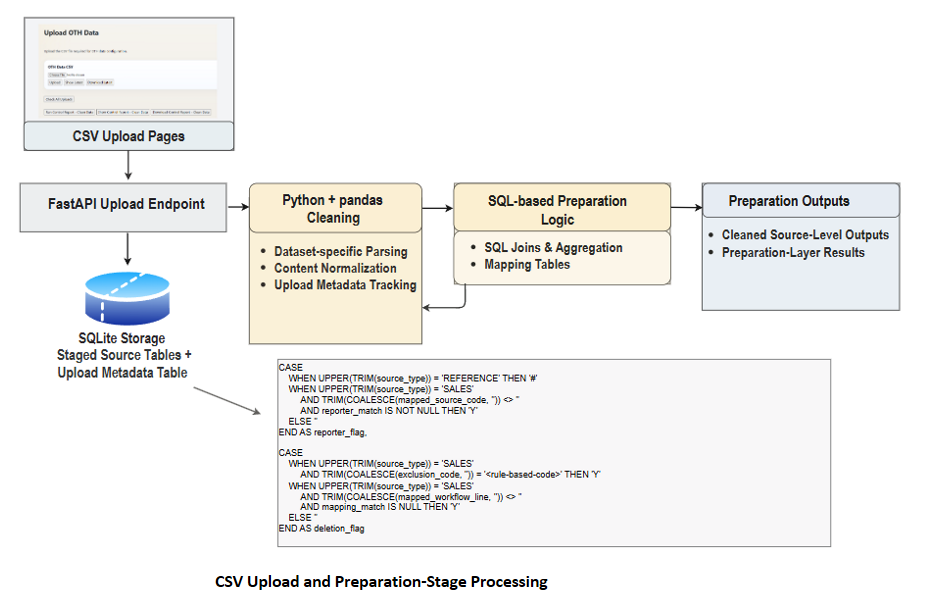
\includegraphics[width=1.1\linewidth]{5.4.png}
%     \caption{Implementation of CSV Upload and Preparation-Stage Processing}
%     \label{fig:5.4}
% \end{figure}

% \begin{figure}[H]
%     \centering
%     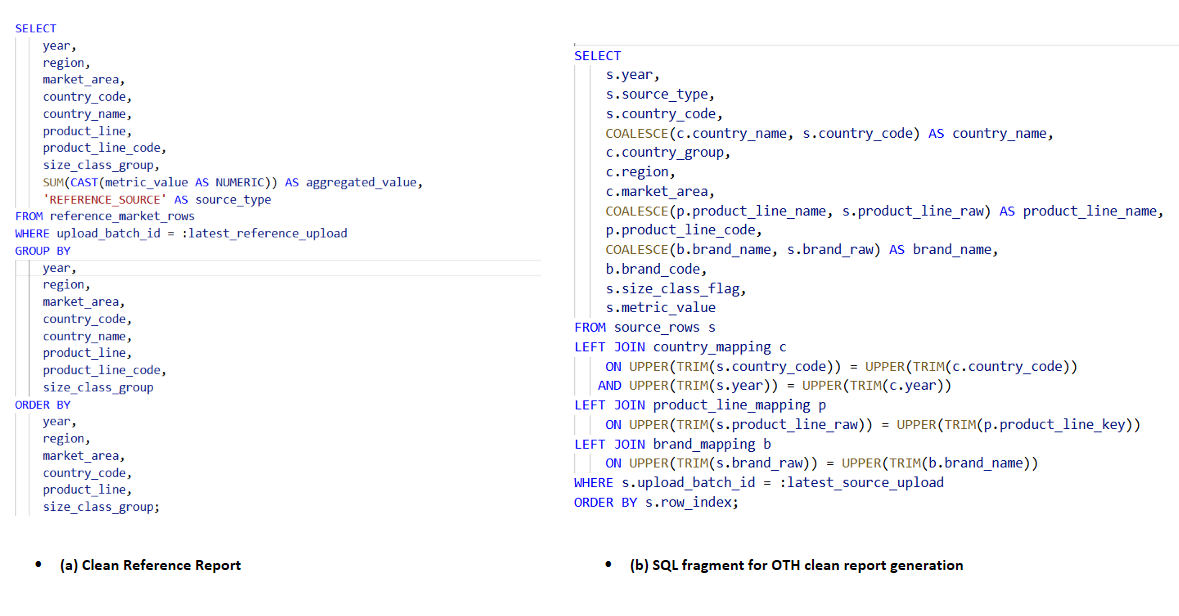
\includegraphics[width=1.1\linewidth]{5.4.1.png}
%     \caption{Simplified SQL Fragments for CRP/TMA and OTH Clean Report Generation}
%     \label{fig:5.4.1}
% \end{figure}

% The preparation stage was then implemented using SQL-based joins, filtering, and aggregation over stored tables. Source records are aligned with mapping data and enriched with workflow control fields such as deletion and reporter flags. The resulting outputs provide a consistent structure for joint inspection of TMA, sales, and OTH data.

% Subsequently, adjustment and prepared result layers were introduced through grouped SQL queries. A key design decision was to return both source-detail rows and derived results within the same output, allowing the frontend to expose how final values are constructed.

% The split stage was implemented by combining prepared OTH data with market-view outputs. Backend logic coordinates the execution, while SQL-derived reference values are used to calculate redistribution ratios. The resulting outputs include summary rows, detailed split results, and supporting reference values, enabling the split logic to be inspected rather than hidden.

% \begin{figure}[H]
%     \centering
%     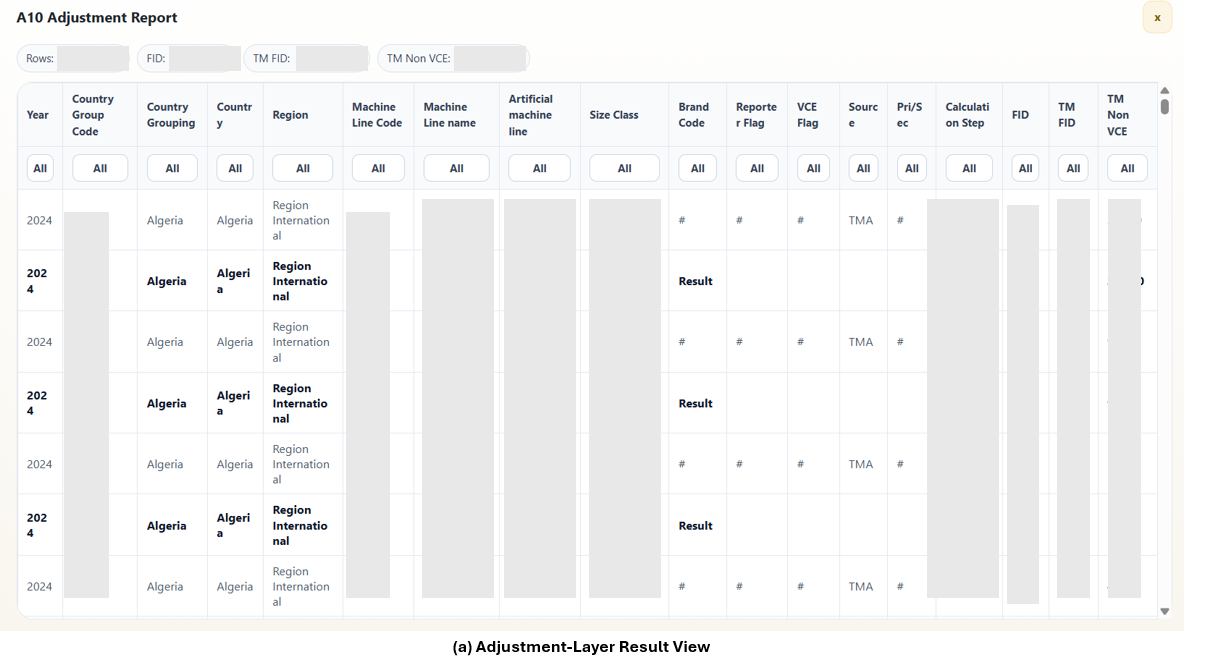
\includegraphics[width=1.1\linewidth]{5.6.1.1.png}
%     \caption{Adjustment-Layer Result View}
%     \label{fig:adjustment-layer-view}
% \end{figure}


% \begin{figure}[H]
%     \centering
%     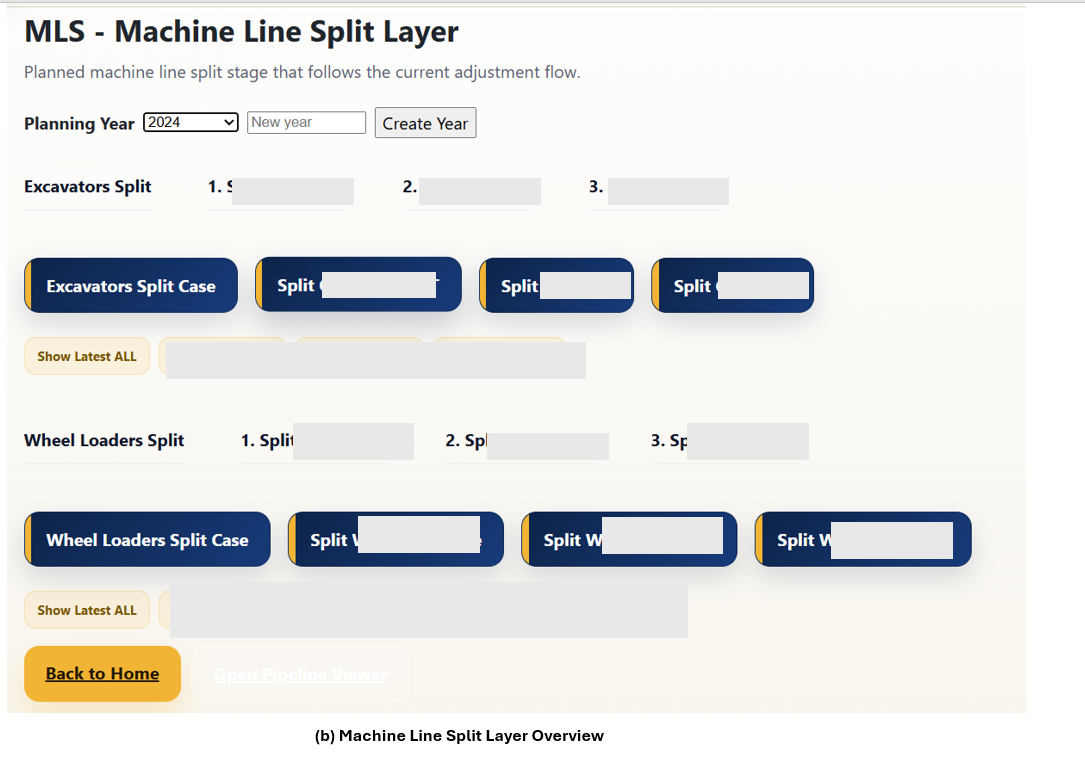
\includegraphics[width=1.1\linewidth]{5.6.1.2.png}
%     \caption{Machine Line Split Layer Overview}
%     \label{fig:split-layer-overview}
% \end{figure}


% \begin{figure}[H]
%     \centering
%     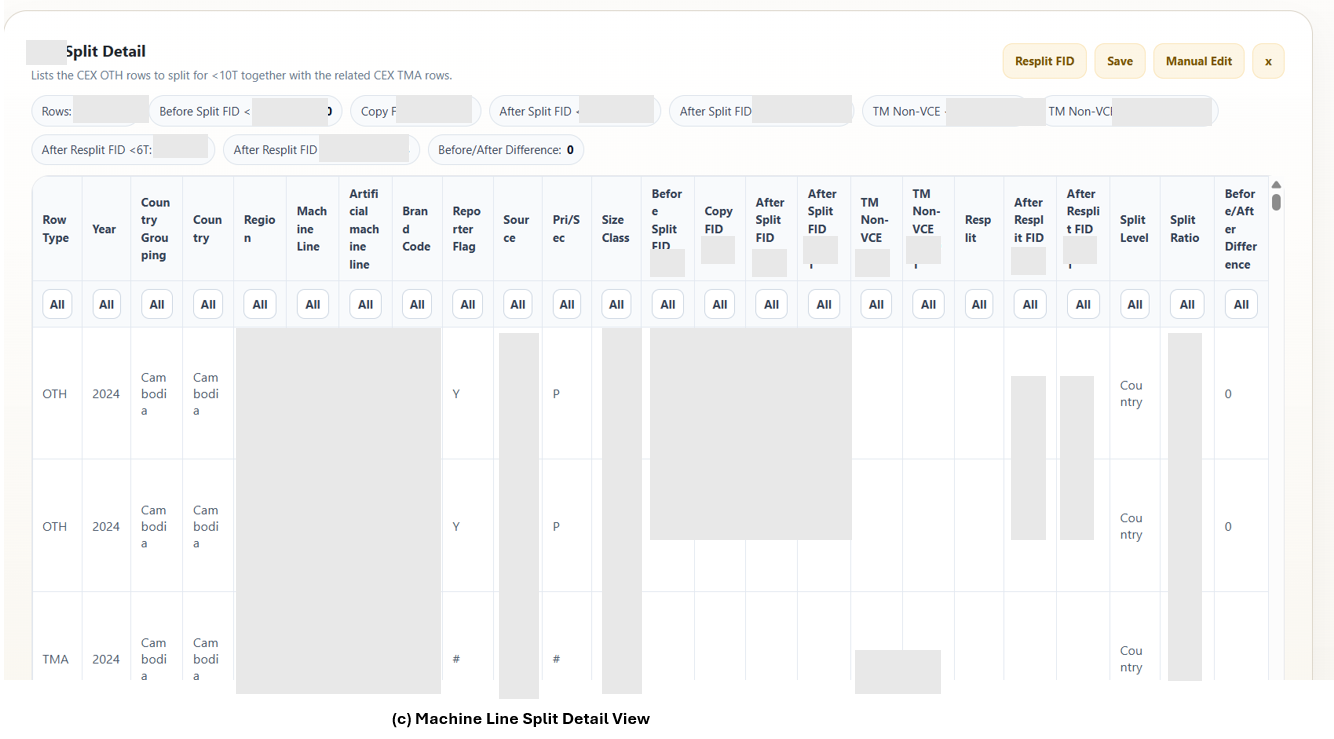
\includegraphics[width=1.1\linewidth]{5.6.1.3.png}
%     \caption{Machine Line Split Detail View}
%     \label{fig:split-detail-view}
% \end{figure}



% \begin{figure}[H]
%     \centering
%     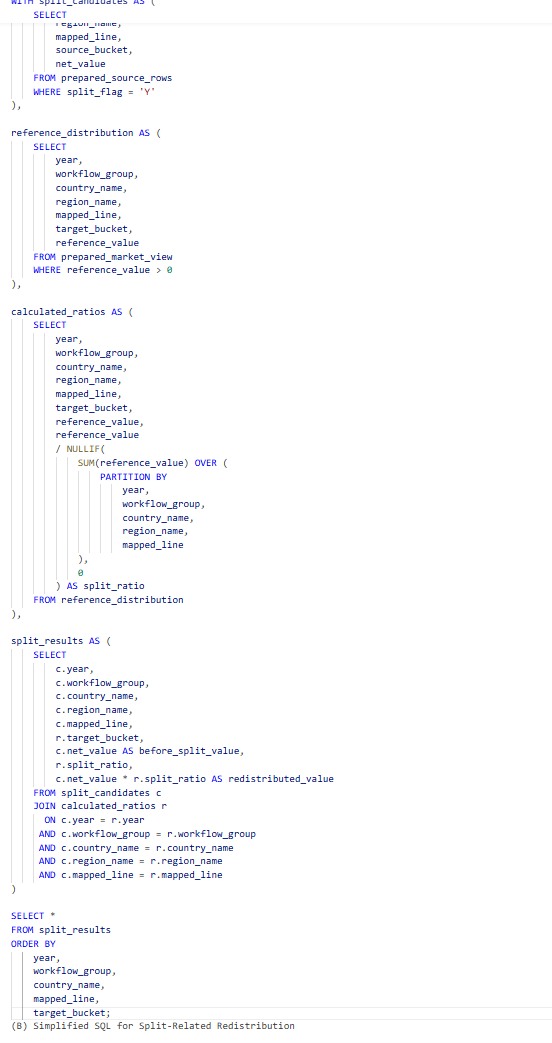
\includegraphics[width=0.85\linewidth]{5.6.4.png}
%     \caption{SQL fragments for adjustment- and split-related processing}
%     \label{fig:sql-fragments-adjustment-split}
% \end{figure}




% Frontend development progressed alongside backend reports. Report endpoints return structured JSON data, which is rendered in workflow-specific views. A reusable filterable table component supports column-based filtering and dynamic aggregation, while summary cards, charts, and CSV export provide both detailed and high-level inspection.


\section{Implementation}

The prototype was implemented as a full-stack web application in which frontend actions trigger backend workflow execution through API-based processing. The implementation followed an incremental structure: authentication, routing, CSV upload, database persistence, and intermediate report generation were established first, after which workflow-specific calculation stages were added. This made it possible to validate each part of the execution chain separately before integrating them into the broader workflow.

At a high level, the frontend acts as the orchestration and inspection layer, while the backend performs data ingestion, workflow processing, and persistence. CSV uploads are normalized into structured relational tables, after which SQL-based transformations and Python-based processing generate preparation, adjustment, and split and resplit outputs. The resulting rows are returned to the frontend as structured JSON and rendered in workflow-specific views for inspection, filtering, aggregation, and export.

\begin{figure}[H]
    \centering
    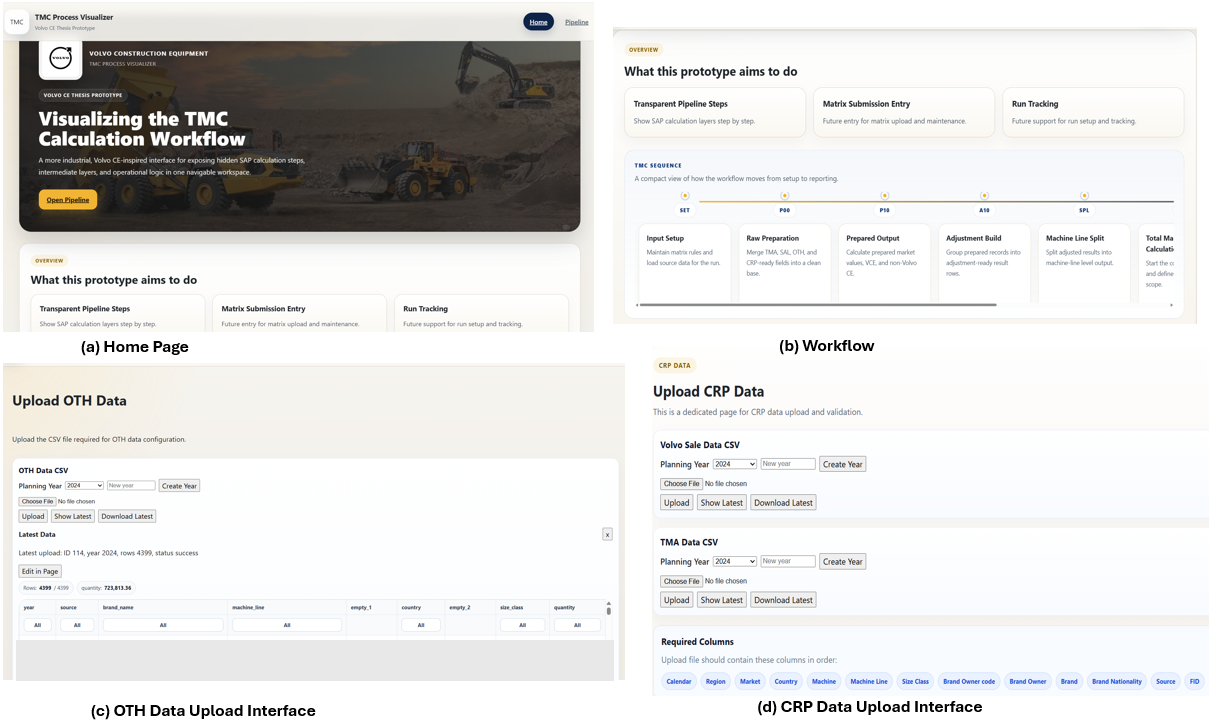
\includegraphics[width=1.05\linewidth]{5.3.1.png}
    \caption{Selected frontend views developed during the implementation of the prototype}
    \label{fig:5.3-main}
\end{figure}

The implementation also established a clear upload-to-processing chain. Files are submitted from the frontend together with dataset type information, processed by dataset-specific handlers, and stored together with upload metadata so that the latest successful input for each dataset can be reused in later workflow steps.

\begin{figure}[H]
    \centering
    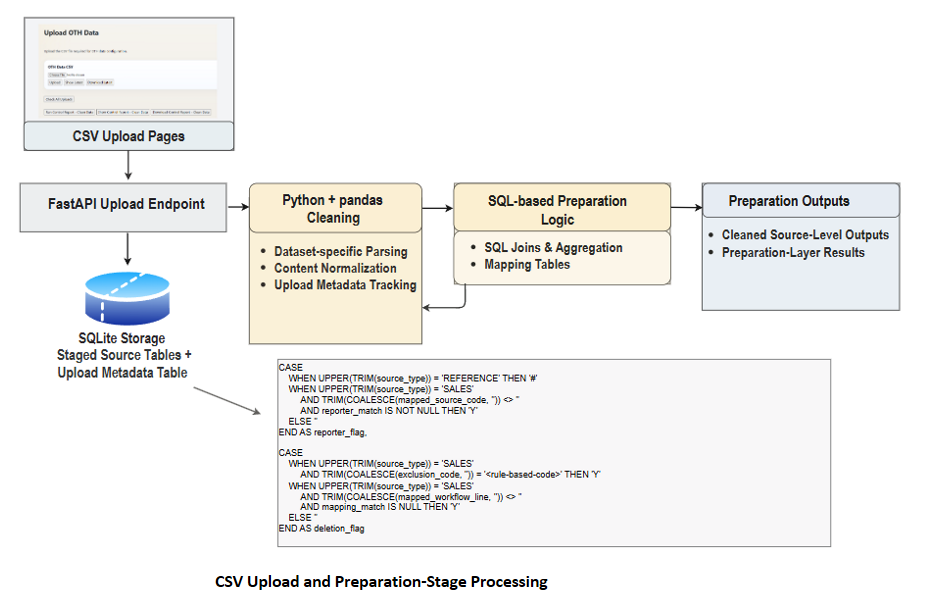
\includegraphics[width=1.05\linewidth]{5.4.png}
    \caption{Implementation of CSV upload and preparation-stage processing}
    \label{fig:5.4-main}
\end{figure}

Once the upload layer was established, the implementation was extended with workflow-specific result layers. In particular, the adjustment and split and resplit views were designed to expose intermediate rows and derived outputs in a form that business users could review directly in the browser.

\begin{figure}[H]
    \centering
    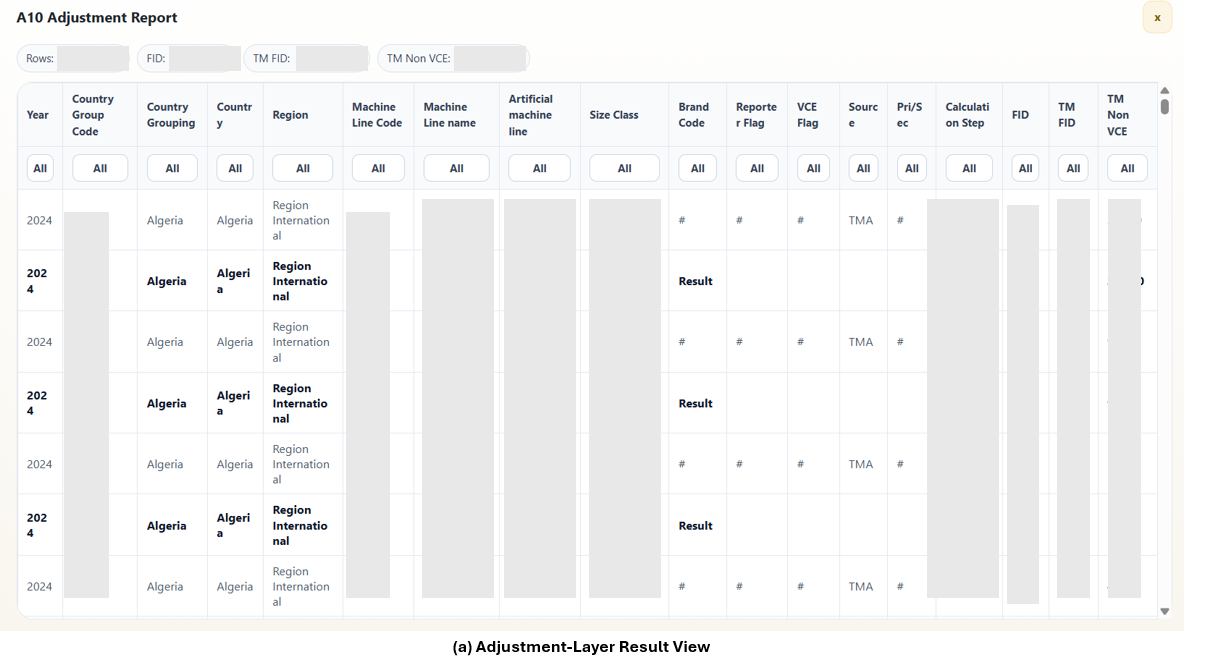
\includegraphics[width=1.05\linewidth]{5.6.1.1.png}
    \caption{Adjustment-layer result view}
    \label{fig:adjustment-layer-main}
\end{figure}

This implementation structure is important because it turns previously embedded workflow logic into explicit and reviewable processing steps. Instead of discussing each technical component in detail in the main body, the thesis focuses here on the design logic and its relation to transparency and inspectability. More detailed implementation notes, example interface views, and supplementary processing fragments are provided in Appendix~\ref{app:supplementary-material}.





% % !TEX root = ../Thesis.tex
% \chapter{Demonstration and Evaluation} 
% \label{cha:Evaluation}




% \section{Demonstration of the Artefact}


% The artefact was demonstrated using real workflow data from the year 2024 calculation cycle in order to evaluate its implemented workflow stages and inspectable outputs. The demonstration covered the deployed prototype setting, execution of the workflow in the web-based environment, and validation of selected outputs against manually verified 2024 results.


% \subsection{Setup of Test Environment}



% For the demonstration, the artefact was operated as a browser-accessible prototype in a \textit{controlled deployment environment}. The frontend, backend, and database layer were run together as one integrated web-based system, allowing users to access the workflow through the implemented interface rather than through local development views alone.

% The evaluation dataset consisted of real workflow data from the \textit{2024 calculation cycle}. This included OTH data, CRP and SAL related reference data, Volvo CE sales data, and matrix-based business input such as source matrix together with related mapping files. These datasets were used as the input basis for evaluating the implemented \textit{preparation}, \textit{adjustment}, and \textit{split-related} logic.


% % \subsection{Execution with Uploaded Workflow Data}

% % In the demonstration, source matrix CSV, CRP and SAL CSV files, and OTH CSV files were submitted through the implemented upload pages of the prototype. The uploaded files were processed successfully and could be displayed again through the corresponding frontend views and report tables.

% % This execution step showed that the prototype could handle heterogeneous CSV input in a consistent way. The implemented parsing logic supported normalization of column names and values, recognition of different header styles, handling of repeated header-like rows, and correct assignment of uploaded values to the expected workflow columns. As a result, the uploaded rows could be aligned reliably with the internal report structure used in later workflow stages.

% % The processed data was then available through filterable tables in the frontend, where rows and columns could be inspected directly. In addition, the prototype supported CSV download of complete generated result tables, allowing the exported outputs to be checked outside the web interface.



% % \subsection{Execution with Uploaded Workflow Data}

% % In the demonstration, the required workflow inputs were uploaded through the implemented frontend pages, including Source Matrix CSV, Reporter List CSV, Size Class CSV, Brand Mapping CSV, Group Country CSV, Machine Line Mapping CSV, OTH data, and CRP-related data. The upload views showed the availability of the required input categories, and each upload could be followed by showing the latest stored version or downloading the latest file from the interface.

% % The uploaded 2024 files were displayed correctly after submission, and the downloaded files matched the expected content without formatting issues or character corruption. The prototype also allowed edited upload data to be saved and downloaded again, and the resulting files remained consistent with the expected output. This confirmed that the upload, display, download, and save functionality worked correctly for the tested 2024 workflow inputs.

% % For the uploaded OTH and CRP data, the cleaned outputs were compared with the corresponding 2024 SAP export tables. The SQL-based cleaning and matching logic produced the expected values, including correct alignment of fields such as country name and market area. The comparison showed that the generated tables were consistent with the SAP reference data, indicating that the upload and initial data-processing steps behaved as intended within the scope of the evaluation.



% \subsection{Execution with Uploaded Workflow Data}

% After the test environment had been prepared, the prototype was executed with the selected 2024 TMC workflow data. The execution followed the implemented workflow sequence from file upload and backend processing to preparation, adjustment, market-view generation, split/resplit processing, and output review.

% The generated outputs were presented through filterable tables, summary views, charts, and CSV export functions. Table~\ref{tab:execution_outputs} summarises the execution steps and main outputs.

% \begin{longtable}{|>{\raggedright\arraybackslash}p{1.0cm}|>{\raggedright\arraybackslash}p{4.6cm}|>{\raggedright\arraybackslash}p{7.8cm}|}
% \caption{Execution flow and main outputs}
% \label{tab:execution_outputs} \\
% \hline
% \textbf{Step} & \textbf{Execution Activity} & \textbf{Main Output Produced} \\
% \hline
% \endfirsthead

% \hline
% \textbf{Step} & \textbf{Execution Activity} & \textbf{Main Output Produced} \\
% \hline
% \endhead

% 1 & Upload source and matrix files & Stored workflow inputs, including Source Matrix, Reporter List, Size Class, Brand Mapping, Group Country, and Machine Line Mapping, with display and download functions. \\
% \hline

% 2 & Upload and register CRP/TMA/SAL/OTH input data & Stored CRP- and TMA-related files, Volvo Sales data, and OTH data as executable workflow inputs for downstream stages. \\
% \hline

% 3 & Generate OTH deletion and reporter base input & Row-level OTH base records with deletion indicators, reporter indicators, source-related fields, and summary values. \\
% \hline

% 4 & Run preparation-stage processing & Cleaned, mapped, and aggregated preparation outputs with mapped dimensions, reporter/deletion fields, and stage-level intermediate results. \\
% \hline

% 5 & Generate market-view and VCE / Non-VCE results & Market-view outputs showing Total Market, Volvo CE, Non-Volvo CE values, summary cards, and ratio-related values. \\
% \hline

% 6 & Run adjustment-stage processing & Adjustment-layer tables with grouped and derived values for intermediate workflow review. \\
% \hline

% 7 & Execute split and resplit logic & Split and resplit outputs with split level, split ratio, before/after values, redistributed rows, and case-related results. \\
% \hline

% 8 & Inspect and export outputs & Filterable stage views, summary views, chart-based review, and CSV export files for comparison and evaluation. \\
% \hline

% \end{longtable}

% % This execution demonstrated how the prototype moves from uploaded source and matrix files to staged preparation, adjustment, split, and export outputs. The generated outputs were then used as the basis for the validation and requirement-based evaluation in the following sections.

% % \section{Evaluation of the Artefact}


% % The artefact was evaluated against the requirements defined in Section~\ref{sec:requirements}. The evaluation assessed both the correctness of the generated outputs and the extent to which the prototype fulfilled the functional, structural, performance, quality, and environmental requirements.

% % The evaluation therefore combined output validation with requirement-based assessment. The generated results were checked against expected business rules and, where comparable, 2024 SAP reference outputs. The requirement-based assessment focused on transparency, traceability, usability, validation support, and prototype-level performance within the selected workflow scope.


% % \subsection{Validation of Prototype Outputs}

% % The generated prototype outputs were validated against the expected workflow logic and, where comparable, against 2024 SAP reference outputs. This validation focused on whether the SQL-based processing produced correct cleaned, mapped, aggregated, split, and resplit-related outputs within the implemented workflow scope.

% % For the preparation stage, validation focused on row counts, mapped fields, reporter and deletion-related flags, aggregated values, and VCE / Non-VCE market-view calculations. For the split and resplit stages, validation focused on whether the prototype identified the correct split records, assigned the expected split levels and split ratios, redistributed values according to the defined business rules, and preserved before- and after-split totals. The detailed validation results are presented in the following subsections.






% % % \subsection{Preparation-Stage Validation}

% % % The preparation stage was evaluated by comparing the generated prototype outputs with workflow data from the 2024 calculation cycle that had already been manually checked. 

% % % For the CRP/TMA- and sales-related preparation outputs, the comparison examined whether the implemented preparation logic produced the expected workflow control fields and grouped values. In particular, the generated deletion flag and reporter flag were checked against the corresponding verified 2024 reference results. The comparison showed that these preparation-related outputs were consistent with the manually verified 2024 data.

% % % For OTH-related preparation, the evaluation focused on whether uploaded source rows were correctly aligned with the relevant mapping structures and then aggregated into the expected preparation-level outputs. In this stage, the mapped OTH values, including brand-related aggregated results, were displayed in the frontend tables and compared with the corresponding manually verified 2024 reference data. The comparison confirmed that the implemented OTH mapping and aggregation logic produced results consistent with the verified 2024 outputs.

% % % The preparation-stage evaluation also included inspection of the frontend-based market-view representation. The VCE and Non-VCE chart was rendered correctly and displayed the expected percentage distribution between the two value categories. In addition, the chart and summary values responded correctly to frontend filtering, and the displayed percentages and totals remained consistent with the filtered result set.


% % % \subsection{Validation of Adjustment- and Split-Related Results}

% % % After the preparation-stage outputs had been validated, the adjustment- and split-related results were evaluated through comparison with manually verified 2024 reference data. This validation focused on whether the implemented later-stage workflow logic produced outputs consistent with the expected 2024 results.

% % % For the adjustment stage, the generated output was compared with the corresponding manually verified 2024 result structure. The comparison showed that the grouped values, source-detail rows, and derived result rows generated by the prototype were consistent with the expected adjustment-related outputs within the scope of the implementation. The frontend representation also allowed these result rows to be inspected directly, making it possible to review how the adjustment output had been formed.

% % % For the split-related stage, validation focused on whether grouped values were redistributed into the expected more detailed result structures. In particular, the evaluation examined the calculated split ratios and the resulting redistributed values. These were compared with the corresponding manually verified 2024 split results. The comparison indicated that the implemented split ratios and the resulting split outputs were consistent with the expected reference results within the scope of the prototype.

% % % The split-related frontend views also supported direct inspection of both summary rows and detailed split rows, including the values before and after redistribution. 


% % % \subsection{Validation of Split- and Resplit-Related Results}

% % % The split- and resplit-related functionality was validated in two steps. First, the number of rows requiring split in the Excavators Split Case and Wheel Loaders Split Case was calculated and compared with the corresponding 2024 SAP records. This check was used to confirm that the prototype identified the same machine-line records as the reference system. In the tested cases, the resulting split row counts and machine-line assignments were consistent with the 2024 SAP outputs.

% % % Second, approximately 20\% of the resulting rows were manually spot-checked in more detail. For these sampled records, the Split Level and Split Ratio values were compared with the corresponding SAP-generated records and with the expected values defined by the split rules. The comparison showed that the prototype produced values consistent with both the SAP reference data and the defined business rules.

% % % Overall, the evaluation indicated that the split and resplit logic behaved as expected within the scope of the tested 2024 cases. The generated outputs matched the reference records, and the detailed sampled checks confirmed that the redistributed values followed the intended split definitions.




% % % \subsection{Preparation-Stage Validation}

% % % The preparation stage was validated by comparing the generated prototype outputs with the corresponding 2024 SAP reference data. The evaluation focused on whether the cleaned and mapped preparation outputs preserved the expected workflow structure, correctly assigned the relevant control fields, and produced row counts and aggregated values consistent with the reference system.

% % % For the CRP-related preparation output, the prototype was checked against the expected reporter classification and grouped preparation structure. In the tested 2024 data, the number of CRP rows identified as reporter rows was 338, which matched the corresponding SAP reference result. In addition, the deletion-related logic was checked to ensure that rows flagged for exclusion were treated consistently with the SAP output.

% % % For the OTH-related preparation output, the cleaned rows were compared with the SAP export to verify that the mapping logic produced the expected field values. In particular, fields such as country name and market area were checked against the corresponding SAP-generated tables, and the resulting outputs were found to be consistent. The evaluation also confirmed that the OTH Reporter Flag was assigned correctly, with 3,407 rows matching the expected reporter classification in the tested 2024 data.

% % % The preparation-stage validation also included the generated VCE / Non-VCE market view. Approximately 20\% of the resulting rows were manually spot-checked to verify that, for each tested country and machine-line combination, the TMA value was correctly reduced by the corresponding Volvo sales value and that the resulting VCE / Non-VCE ratio was displayed correctly. The checked records were consistent with the expected calculations, confirming that the prototype produced the intended market-share representation for the tested 2024 data.

% % % Overall, the preparation-stage validation showed that the prototype produced cleaned, mapped, and aggregated outputs consistent with the 2024 SAP reference data. The row counts, control flags, key mapped fields, and market-view calculations all matched the expected values, indicating that the implemented preparation logic behaved correctly within the scope of the evaluation.

% % \subsection{Preparation-Stage Validation}

% % The preparation stage was evaluated through data comparison and output inspection. The purpose of this validation was to assess whether the prototype generated preparation outputs that were consistent with the expected workflow logic and the corresponding 2024 SAP reference data. The evaluation parameters included row-count consistency, correctness of mapped fields, correctness of workflow control flags, and correctness of the VCE / Non-VCE market-view calculation.

% % For the CRP-related preparation output, the prototype result was compared with the expected reporter classification and grouped preparation structure from the SAP reference data. In the tested 2024 data, the number of CRP rows identified as reporter rows was 338, which matched the corresponding SAP reference result. The deletion-related logic was also checked to verify that rows flagged for exclusion were treated consistently with the SAP output.

% % For the OTH-related preparation output, the cleaned and mapped rows were compared with the SAP export tables. The comparison focused on whether key mapped fields, such as country name and market area, were aligned with the SAP-generated values. The generated outputs were consistent with the SAP reference data. The OTH Reporter Flag was also assigned correctly, with 3,407 rows matching the expected reporter classification in the tested 2024 data.

% % The preparation-stage validation further included the generated VCE / Non-VCE market view. Approximately 20\% of the resulting rows were manually spot-checked across selected country and machine-line combinations. For each checked record, the validation examined whether the TMA value was correctly reduced by the corresponding Volvo CE sales value and whether the resulting VCE / Non-VCE ratio was displayed correctly. The checked records were consistent with the expected calculations.



% % % \subsection{Validation of Split- and Resplit-Related Results}

% % % The split- and resplit-related functionality was validated in two steps. First, the number of rows requiring split in the Excavators Split Case and Wheel Loaders Split Case was calculated and compared with the corresponding 2024 SAP records. This check was used to verify that the prototype identified the same machine-line records as the reference system. In the tested cases, the resulting split row counts and machine-line assignments were consistent with the 2024 SAP outputs.

% % % Second, approximately 20\% of the resulting rows were manually spot-checked in more detail. The sampled records were selected from different country and machine-line combinations to ensure that the validation covered representative split patterns. For each sampled row, the Split Level, Split Ratio, and redistributed values were compared with both the SAP-generated records and the expected values defined by the split rules. In addition, the before-split and after-split values were checked to confirm that the redistribution followed the intended business logic and preserved the original totals.

% % % The same validation approach was applied to the resplit functionality. In this case, the resplit logic was guided by a manual business-rule check of whether a brand was actually sold in the relevant country or region for the affected machine line. If one of the finer target categories did not exist for that brand in the given market, the corresponding value was reassigned to the remaining valid category. In practice, the resplit logic redistributed the value into two finer buckets, ensuring that the value of the missing bucket was moved to the existing one according to the resplit rules. A similar spot-check was then applied to approximately 20\% of the resplit rows. The sampled records were compared with the corresponding SAP outputs and with the expected business-rule outcome for the relevant brand and region, and the results were consistent in the tested cases.

% % % Overall, the evaluation showed that the prototype produced split and resplit outputs consistent with the 2024 SAP reference data. The row selection, split assignment, and redistribution logic were consistent with the expected machine-line records, and the sampled detailed checks confirmed that the implemented behaviour matched the business rules within the scope of the tested cases.




% % \subsection{Split- and Resplit-Related Validation}

% % The split- and resplit-related outputs were evaluated through comparison with 2024 SAP reference records and manual output inspection. The validation focused on four parameters: correct identification of records requiring split, correctness of split level and split ratio assignment, correctness of redistributed values, and preservation of before- and after-split totals.

% % For the split functionality, the number of rows requiring split in the Excavators Split Case and Wheel Loaders Split Case was calculated and compared with the corresponding 2024 SAP records. This check verified whether the prototype identified the same machine-line records as the reference system. In the tested cases, the split row counts and machine-line assignments were consistent with the SAP outputs. Approximately 20\% of the resulting split rows were then manually spot-checked across different country and machine-line combinations. For each sampled row, the split level, split ratio, redistributed values, and before- and after-split totals were compared with the SAP-generated records and the expected values defined by the split rules.

% % The same validation approach was applied to the resplit functionality. The resplit logic was checked against the business rule that invalid brand--machine-line--size-class combinations should be removed and redistributed to the remaining valid categories. Approximately 20\% of the resplit rows were manually spot-checked and compared with the corresponding SAP outputs and expected business-rule outcomes. The sampled results were consistent in the tested cases, indicating that the implemented split and resplit logic behaved correctly within the evaluated scope.

% % During the split validation, one discrepancy was also observed between the currently expected split logic and the corresponding SAP output. According to the business interpretation used in the prototype, machine-line split for non-VCE reporter-brand values should be based on the distribution of non-VCE TMA values across the relevant finer size classes. Since the split is applied to non-VCE values, Volvo CE volume should be excluded from TMA before calculating the split ratio. However, in one reviewed SAP case, the observed split ratio appeared to be calculated from total TMA values including Volvo CE volume. This produced a different allocation compared with the non-VCE-based split ratio implemented in the prototype.

% % This discrepancy suggests that the SAP output may reflect historical calculation logic or an implementation detail that is not fully aligned with the currently expected business rule. It was therefore not treated simply as a prototype error, but as an important validation finding. The case demonstrates how making intermediate split ratios and rule applications visible can support discussion and clarification of business rules that are otherwise difficult to inspect in the SAP-based workflow.



% \section{Evaluation of the Artefact}

% The artefact was evaluated against the requirements defined in Section~\ref{sec:requirements}. The evaluation combined output validation with requirement-based assessment. Output validation examined whether the generated results were consistent with expected business rules and, where comparable, with 2024 SAP reference outputs. Requirement-based assessment examined whether the prototype fulfilled the functional, structural, performance, quality, and environmental requirements, with particular attention to transparency, traceability, usability, validation support, and prototype-level performance.

% \subsection{Validation of Prototype Outputs}

% The generated prototype outputs were validated against the expected workflow logic and, where comparable, against 2024 SAP reference outputs. The validation used comparison-based parameters to assess whether the SQL-based processing produced correct cleaned, mapped, aggregated, split, and resplit-related outputs within the implemented workflow scope.

% For the preparation stage, the validation parameters were:
% \begin{itemize}
%     \item row-count consistency;
%     \item mapped-field consistency;
%     \item workflow control-flag correctness;
%     \item aggregated-value consistency;
%     \item correctness of the VCE / Non-VCE market-view calculation.
% \end{itemize}

% For the split and resplit stages, the validation parameters were:
% \begin{itemize}
%     \item correct identification of records requiring split;
%     \item correctness of split level and split ratio assignment;
%     \item correctness of redistributed values;
%     \item preservation of before- and after-split totals.
% \end{itemize}

% The detailed validation results are presented in the following subsections.

% \subsection{Preparation-Stage Validation}

% The preparation stage was evaluated through comparison with 2024 SAP reference data and manual output inspection. The purpose was to assess whether the generated preparation outputs were consistent with the expected workflow logic.

% For the CRP-related preparation output, the prototype result was compared with the expected reporter classification and grouped preparation structure from the SAP reference data. In the tested 2024 data, 338 CRP rows were identified as reporter rows, matching the corresponding SAP reference result. The deletion-related logic was also checked to verify that rows flagged for exclusion were treated consistently with the SAP output.

% For the OTH-related preparation output, the cleaned and mapped rows were compared with SAP export tables. Key mapped fields, such as country name and market area, were aligned with the SAP-generated values. The OTH Reporter Flag was also assigned correctly, with 3,407 rows matching the expected reporter classification in the tested 2024 data.

% The preparation-stage validation further included the generated VCE / Non-VCE market view. Approximately 20\% of the resulting rows were manually spot-checked across selected country and machine-line combinations. For each checked record, the validation examined whether the TMA value was correctly reduced by the corresponding Volvo CE sales value and whether the resulting VCE / Non-VCE ratio was displayed correctly. The checked records were consistent with the expected calculations.

% Overall, the preparation-stage validation showed that the prototype produced cleaned, mapped, and aggregated outputs consistent with the 2024 SAP reference data and expected business logic within the tested scope.

% \subsection{Split- and Resplit-Related Validation}

% The split- and resplit-related outputs were evaluated through comparison with 2024 SAP reference records and manual output inspection. The validation focused on split-record identification, split-level and split-ratio correctness, redistributed-value correctness, and preservation of before- and after-split totals.

% For the split functionality, the number of rows requiring split in the Excavators Split Case and Wheel Loaders Split Case was calculated and compared with the corresponding 2024 SAP records. This check verified whether the prototype identified the same machine-line records as the reference system. In the tested cases, the split row counts and machine-line assignments were consistent with the SAP outputs. Approximately 20\% of the resulting split rows were then manually spot-checked across different country and machine-line combinations. For each sampled row, the split level, split ratio, redistributed values, and before- and after-split totals were compared with the SAP-generated records and the expected values defined by the split rules.

% The same validation approach was applied to the resplit functionality. The resplit logic was checked against the business rule that invalid brand--machine-line--size-class combinations should be removed and redistributed to the remaining valid categories. Approximately 20\% of the resplit rows were manually spot-checked and compared with the corresponding SAP outputs and expected business-rule outcomes. The sampled results were consistent in the tested cases, indicating that the implemented split and resplit logic behaved correctly within the evaluated scope.

% \paragraph{Observed discrepancy in split logic.}
% During the split validation, one discrepancy was also observed between the currently expected split logic and the corresponding SAP output. According to the business interpretation used in the prototype, machine-line split for non-VCE reporter-brand values should be based on the distribution of non-VCE TMA values across the relevant finer size classes. Since the split is applied to non-VCE values, Volvo CE volume should be excluded from TMA before calculating the split ratio. However, in one reviewed SAP case, the observed split ratio appeared to be calculated from total TMA values including Volvo CE volume. This produced a different allocation compared with the non-VCE-based split ratio implemented in the prototype.

% This discrepancy suggests that the SAP output may reflect historical calculation logic or an implementation detail that is not fully aligned with the currently expected business rule. It was therefore not treated simply as a prototype error, but as an important validation finding. The case demonstrates how making intermediate split ratios and rule applications visible can support discussion and clarification of business rules that are otherwise difficult to inspect in the SAP-based workflow.



% \section{Evaluation Against Requirements}

% The artefact was further evaluated against the requirements defined in Section~\ref{sec:requirements}. To make the assessment explicit, each requirement was linked to an evaluation parameter or metric and evaluated using evidence from the prototype functions, generated outputs, validation checks, and stakeholder feedback.

% SAP reference outputs were used where direct comparison was possible, particularly for validating preparation-, split-, and resplit-related results. However, not all evaluation parameters could be assessed through direct SAP comparison. Transparency, traceability, and usability were evaluated mainly through the implemented prototype functions, the visibility of intermediate outputs, the availability of source and rule context fields, and stakeholder feedback during prototype review. Performance and stability were assessed at prototype level through observed execution and repeated review operations in the test environment.

% The results are summarised in Table~\ref{tab:evaluation_parameters}.

% \begin{longtable}{|>{\raggedright\arraybackslash}p{1.2cm}|>{\raggedright\arraybackslash}p{2.7cm}|>{\raggedright\arraybackslash}p{4.0cm}|>{\raggedright\arraybackslash}p{6.0cm}|}
% \caption{Evaluation against requirements}
% \label{tab:evaluation_parameters} \\
% \hline
% \textbf{ID} & \textbf{Evaluation Dimension} & \textbf{Evaluation Parameter / Metric} & \textbf{Evidence and Evaluation Result} \\
% \hline
% \endfirsthead

% \hline
% \textbf{ID} & \textbf{Evaluation Dimension} & \textbf{Evaluation Metric} & \textbf{Evidence and Evaluation Result} \\
% \hline
% \endhead

% FR1 & Functional fulfilment & Completion of source and matrix file upload and management. & CSV-based source data and matrix files were uploaded through the frontend pages. The uploaded files could be displayed, stored, downloaded, and reused in later workflow stages. \\
% \hline

% FR2 & Functional fulfilment & Successful execution of backend workflow processing. & Backend processing re-expressed selected SAP-based TMC workflow logic, including preparation, adjustment, and split-related processing. The generated outputs were used for validation against expected business rules and, where comparable, SAP reference outputs. \\
% \hline

% FR3 & Functional fulfilment / usability & Availability of frontend review functions. & The prototype provided filterable tables, summary values, chart-based review, and CSV export. These functions allowed users to inspect detailed records and aggregated outputs through the browser interface. \\
% \hline

% SR1 & Structural fit & Separation of upload, processing, storage, and visualisation components. & The artefact used a modular web-based frontend-backend architecture, with frontend views, backend services, and relational database storage separated into different components. \\
% \hline

% SR2 & Structural fit & Structured storage of uploaded files, mappings, workflow records, and generated outputs. & Uploaded files, mapping data, intermediate workflow records, and generated outputs were stored in structured form, supporting repeated review and future extension to later workflow stages. \\
% \hline

% PR1 & Performance & Successful completion of stage and report execution for the selected 2024 dataset. & Demonstration runs using the selected 2024 TMC data completed within a practically acceptable time for prototype-based review. Formal production-level benchmarking was outside the thesis scope. \\
% \hline

% PR2 & Performance / stability & Absence of crashes, data loss, or inconsistent save/reload behaviour during repeated operations. & Repeated upload, processing, filtering, save/reload, and export operations were performed in the test environment. The prototype remained usable for prototype-level evaluation. \\
% \hline

% QR1 & Transparency & Visibility of intermediate workflow stages, row-level outputs, and stage summaries. & Compared with the SAP-based representation, the prototype exposed preparation, adjustment, split, and resplit-related outputs as separate inspectable stages. Row-level tables and summaries allowed users to review how values were formed step by step within the implemented scope. \\
% \hline

% QR2 & Traceability & Availability of source, mapping, control-flag, and rule-decision context in generated stage outputs. & Generated outputs preserved relevant stage-level context, including source, country, machine line, brand, reporter flags, deletion flags, split levels, and split ratios. This supported stage-level traceability between input data, rule context, and generated outputs, while full row-level lineage remains future work. \\
% \hline

% QR3 & Usability & Ability to complete BI review tasks through the browser interface with acceptable effort. & Users could navigate workflow stages, inspect records, filter outputs, review summaries and charts, and export CSV files. Stakeholder feedback indicated that these functions were useful for review and validation tasks, although further interface refinement would be needed for broader operational use. \\
% \hline

% ER1 & Environmental fit & Operation in a controlled prototype environment. & The artefact was operated as a browser-accessible prototype using a web frontend, backend service, and relational database. This environment supported demonstration and evaluation with the selected 2024 workflow data. \\
% \hline

% ER2 & Environmental fit & Future adaptability to more robust cloud or Volvo CE internal infrastructure. & The modular architecture provides a basis for future adaptation to more robust cloud deployment or Volvo CE internal infrastructure. Full enterprise integration remains future work. \\
% \hline

% \end{longtable}




% \section{Comparison with the SAP-Based Workflow}

% To further clarify the evaluation of transparency, traceability, usability, validation support, and performance, the prototype was compared with the current SAP-based workflow representation from a business-user perspective. This comparison does not claim that SAP lacks these capabilities technically. Rather, it assesses whether the functions are directly available and inspectable for business users within the reviewed workflow.

% \begin{longtable}{|
% >{\raggedright\arraybackslash}p{2.6cm}|
% >{\raggedright\arraybackslash}p{2.4cm}|
% >{\raggedright\arraybackslash}p{2.4cm}|
% >{\raggedright\arraybackslash}p{6.2cm}|}
% \caption{Comparison between the SAP-based workflow and the prototype from a business-user perspective}
% \label{tab:sap_prototype_comparison} \\
% \hline
% \textbf{Evaluation Dimension} & \textbf{SAP-based Workflow} & \textbf{Prototype} & \textbf{Explanation} \\
% \hline
% \endfirsthead

% \hline
% \textbf{Evaluation Dimension} & \textbf{SAP-based Workflow} & \textbf{Prototype} & \textbf{Explanation} \\
% \hline
% \endhead

% Transparency & Limited for business users & Supported & The prototype exposes preparation, adjustment, split, and resplit outputs as separate inspectable stages. In the SAP-based representation, these workflow layers are not provided in one review-oriented interface for business users. \\
% \hline

% Traceability & Limited for business users & Partly supported & The prototype preserves stage-level source and rule context fields, such as country, machine line, source, brand, flags, split level, and split ratio. Full row-level lineage across all transformations is not yet implemented. \\
% \hline

% Usability & Limited for business users & Supported & The prototype provides browser-based filtering, summaries, chart-based review, and CSV export for BI review tasks. The SAP-based workflow requires more SAP-specific navigation and technical knowledge. \\
% \hline

% Validation support & Limited for business users & Supported & Intermediate outputs, totals, flags, and split ratios can be inspected and compared with expected business rules in the prototype. In the SAP-based workflow, such validation often requires additional extraction or IT-supported investigation. \\
% \hline

% Performance and stability & Not directly compared & Prototype-level support & The prototype completed the selected 2024 workflow runs and remained usable during repeated upload, processing, filtering, save/reload, and export operations. A direct production-level performance comparison with SAP was outside the thesis scope. \\
% \hline

% \end{longtable}














% % \section{Evaluation Against Requirements}

% % The implemented artefact was assessed in relation to the requirements identified in Chapter 4. The outcome of this assessment is summarized in Table 4.1.

% % \begin{table}[H]
% % \centering
% % \begin{tabular}{p{2.5cm} p{10cm}}
% % \hline
% % \textbf{Category} & \textbf{Evaluation Result} \\
% % \hline

% % \textbf{Functional} & The artefact supports structured upload and management of CSV-based source data and matrix files, allowing users to provide the required inputs for the workflow. \\

% % \textbf{Functional} & Key parts of the SAP-based workflow logic were re-expressed through backend processing and staged report generation, making the transformation steps more explicit and easier to follow. \\

% % \textbf{Functional} & Within the scope of the prototype, preparation, adjustment, and split-related stages are represented through inspectable workflow-layer outputs, enabling step-by-step validation. \\

% % \textbf{Functional} & The frontend supports filtering, summary calculation, chart-based inspection, and CSV export, allowing users to explore both detailed records and aggregated results. \\

% % \hline

% % \textbf{Structural} & The artefact is implemented as a web-based system with a clear separation between frontend and backend components. \\

% % \textbf{Structural} & Upload handling, backend processing, and frontend visualization are implemented as separate modules, which improves maintainability and extensibility. \\

% % \textbf{Structural} & Within the prototype scope, the system supports structured storage of workflow data, mappings, and derived outputs, while allowing further extensions. \\

% % \hline

% % \textbf{Environmental} & The artefact provides a more transparent and user-oriented representation compared to the original SAP-based workflow. \\

% % \textbf{Environmental} & Intermediate outputs, totals, and potential data issues can be inspected directly, supporting validation and analysis. \\

% % \textbf{Environmental} & The prototype demonstrates potential for supporting market-related analysis, although full integration into existing enterprise systems remains future work. \\

% % \hline
% % \end{tabular}
% % \caption{Evaluation of artefact requirements}
% % \label{tab:requirement_evaluation_tmc}
% % \end{table}


% \section{Summary and Limitations}

% The evaluation showed that the artefact fulfills its core purpose as a web-based prototype for the TMC workflow. Within the implemented scope, the system supported structured CSV upload, staged backend processing, workflow-layer inspection, and validation of generated outputs against manually verified 2024 reference results.

% Several limitations nonetheless apply:
% \begin{itemize}
% \item The prototype covers only selected stages of the broader TMC process.
% \item The validation was conducted with data from the 2024 calculation cycle, so the results cannot yet be generalised across all years and workflow variations.
% \item The artefact remains sensitive to the structural quality of uploaded CSV files and mapping data, despite the cleaning and normalisation logic that has been implemented.
% \item The current deployment and storage setup is adequate for prototype use, but broader internal deployment would require more robust infrastructure and deeper integration with enterprise systems.
% \end{itemize}

% !TEX root = ../Thesis.tex


% \chapter{Demonstration and Evaluation} 
% \label{cha:Evaluation}

% \section{Demonstration of the Artefact}


% The artefact was demonstrated using real workflow data from the year 2024 calculation cycle in order to evaluate its implemented workflow stages and inspectable outputs. The demonstration covered the deployed prototype setting, execution of the workflow in the web-based environment, and validation of selected outputs against manually verified 2024 results.


% \subsection{Setup of Test Environment}

% For the demonstration, the artefact was operated as a browser-accessible prototype in a \textit{controlled deployment environment}. The frontend, backend, and database layer were run together as one integrated web-based system, allowing users to access the workflow through the implemented interface rather than through local development views alone.

% The evaluation dataset consisted of real workflow data from the \textit{2024 calculation cycle}. This included OTH data, CRP and SAL related reference data, Volvo CE sales data, and matrix-based business input such as source matrix together with related mapping files. These datasets were used as the input basis for evaluating the implemented \textit{preparation}, \textit{adjustment}, and \textit{split-related} logic.

% \subsection{Execution with Uploaded Workflow Data}

% After the test environment had been prepared, the prototype was executed with the selected 2024 TMC workflow data. The execution followed the implemented workflow sequence from file upload and backend processing to preparation, adjustment, market-view generation, split/resplit processing, and output review.

% The generated outputs were presented through filterable tables, summary views, charts, and CSV export functions. Table~\ref{tab:execution_outputs} summarises the execution steps and main outputs.

% \begin{longtable}{|>{\raggedright\arraybackslash}p{1.0cm}|>{\raggedright\arraybackslash}p{4.6cm}|>{\raggedright\arraybackslash}p{7.8cm}|}
% \caption{Execution flow and main outputs}
% \label{tab:execution_outputs} \\
% \hline
% \textbf{Step} & \textbf{Execution Activity} & \textbf{Main Output Produced} \\
% \hline
% \endfirsthead

% \hline
% \textbf{Step} & \textbf{Execution Activity} & \textbf{Main Output Produced} \\
% \hline
% \endhead

% 1 & Upload source and matrix files & Stored workflow inputs, including Source Matrix, Reporter List, Size Class, Brand Mapping, Group Country, and Machine Line Mapping, with display and download functions. \\
% \hline

% 2 & Upload and register CRP/TMA/SAL/OTH input data & Stored CRP- and TMA-related files, Volvo Sales data, and OTH data as executable workflow inputs for downstream stages. \\
% \hline

% 3 & Generate OTH deletion and reporter base input & Row-level OTH base records with deletion indicators, reporter indicators, source-related fields, and summary values. \\
% \hline

% 4 & Run preparation-stage processing & Cleaned, mapped, and aggregated preparation outputs with mapped dimensions, reporter/deletion fields, and stage-level intermediate results. \\
% \hline

% 5 & Generate market-view and VCE / Non-VCE results & Market-view outputs showing Total Market, Volvo CE, Non-Volvo CE values, summary cards, and ratio-related values. \\
% \hline

% 6 & Run adjustment-stage processing & Adjustment-layer tables with grouped and derived values for intermediate workflow review. \\
% \hline

% 7 & Execute split and resplit logic & Split and resplit outputs with split level, split ratio, before/after values, and redistributed rows. \\
% \hline

% 8 & Inspect and export outputs & Filterable stage views, summary views, chart-based review, and CSV export files for comparison and evaluation. \\
% \hline

% \end{longtable}

% \section{Evaluation of the Artefact}

% The artefact was evaluated against the requirements defined in Section~\ref{sec:requirements}. The evaluation combined output validation with requirement-based assessment. Output validation examined whether the generated results were consistent with expected business rules and, where comparable, with 2024 SAP reference outputs. Requirement-based assessment examined whether the prototype fulfilled the functional, structural, performance, quality, and environmental requirements, with particular attention to transparency, traceability, usability, validation support, and prototype-level performance.

% \subsection{Validation of Prototype Outputs}

% The generated prototype outputs were validated against the expected workflow logic and, where comparable, against 2024 SAP reference outputs. The validation used comparison-based parameters to assess whether the SQL-based processing produced correct cleaned, mapped, aggregated, split, and resplit-related outputs within the implemented workflow scope.

% For the preparation stage, the validation parameters were:
% \begin{itemize}
%     \item row-count consistency;
%     \item mapped-field consistency;
%     \item workflow control-flag correctness;
%     \item aggregated-value consistency;
%     \item correctness of the VCE / Non-VCE market-view calculation.
% \end{itemize}

% For the split and resplit stages, the validation parameters were:
% \begin{itemize}
%     \item correct identification of records requiring split;
%     \item correctness of split level and split ratio assignment;
%     \item correctness of redistributed values;
%     \item preservation of before- and after-split totals.
% \end{itemize}

% The detailed validation results are presented in the following subsections.

% \subsection{Preparation-Stage Validation}

% The preparation stage was evaluated through comparison with 2024 SAP reference data and manual output inspection. The purpose was to assess whether the generated preparation outputs were consistent with the expected workflow logic.

% For the CRP-related preparation output, the prototype result was compared with the expected reporter classification and grouped preparation structure from the SAP reference data. In the tested 2024 data, 338 CRP rows were identified as reporter rows, matching the corresponding SAP reference result. The deletion-related logic was also checked to verify that rows flagged for exclusion were treated consistently with the SAP output.

% For the OTH-related preparation output, the cleaned and mapped rows were compared with SAP export tables. Key mapped fields, such as country name and market area, were aligned with the SAP-generated values. The OTH Reporter Flag was also assigned correctly, with 3,407 rows matching the expected reporter classification in the tested 2024 data.

% The preparation-stage validation further included the generated VCE / Non-VCE market view. Approximately 20\% of the resulting rows were manually spot-checked across selected country and machine-line combinations. For each checked record, the validation examined whether the TMA value was correctly reduced by the corresponding Volvo CE sales value and whether the resulting VCE / Non-VCE ratio was displayed correctly. The checked records were consistent with the expected calculations.

% Overall, the preparation-stage validation showed that the prototype produced cleaned, mapped, and aggregated outputs consistent with the 2024 SAP reference data and expected business logic within the tested scope.



% \subsection{Split- and Resplit-Related Validation}

% The split- and resplit-related outputs were validated against 2024 SAP reference records and manual output inspection. The formal evaluation scope of this thesis was limited to workflow stages up to machine line split/resplit. Validation focused on: (1) correct split-row selection, (2) split-level and split-ratio correctness, (3) redistributed-value correctness, and (4) preservation of before/after totals.

% For split validation, row counts for the Excavators Split Case and Wheel Loaders Split Case were compared with SAP reference records. In the tested cases, split-row selection and machine-line assignments were consistent with SAP outputs. Approximately 20\% of resulting split rows were then spot-checked across representative country and machine-line combinations; sampled split levels, split ratios, redistributed values, and totals were consistent with expected rules.

% For resplit validation, approximately 20\% of resplit rows were spot-checked against SAP outputs and expected business-rule outcomes. The sampled cases were consistent within the tested scope.

% \paragraph{Observed discrepancy in split logic.}
% One discrepancy was observed in a reviewed SAP case: the SAP split ratio appeared to be based on total TMA including Volvo CE volume, while the prototype used non-VCE-based split interpretation for non-VCE split values. This finding was treated as a rule-clarification issue rather than a direct prototype failure, and it highlights the value of exposing intermediate split ratios and rule context.


% \section{Evaluation Against Requirements}

% The artefact was further evaluated against the requirements defined in Section~\ref{sec:requirements}. To make the assessment explicit, each requirement was linked to an evaluation parameter or metric and evaluated using evidence from the prototype functions, generated outputs, validation checks, and stakeholder feedback.

% SAP reference outputs were used where direct comparison was possible, particularly for validating preparation-, split-, and resplit-related results. However, not all evaluation parameters could be assessed through direct SAP comparison. Transparency, traceability, and usability were evaluated mainly through the implemented prototype functions, the visibility of intermediate outputs, the availability of source and rule context fields, and stakeholder feedback during prototype review. Performance and stability were assessed at prototype level through observed execution and repeated review operations in the test environment.

% The results are summarised in Table~\ref{tab:evaluation_parameters}.

% \begin{longtable}{|>{\raggedright\arraybackslash}p{1.2cm}|>{\raggedright\arraybackslash}p{2.7cm}|>{\raggedright\arraybackslash}p{4.0cm}|>{\raggedright\arraybackslash}p{6.0cm}|}
% \caption{Evaluation against requirements}
% \label{tab:evaluation_parameters} \\
% \hline
% \textbf{ID} & \textbf{Evaluation Dimension} & \textbf{Evaluation Parameter} & \textbf{Evaluation Result} \\
% \hline
% \endfirsthead

% \hline
% \textbf{ID} & \textbf{Evaluation Dimension} & \textbf{Evaluation Metric} & \textbf{Evaluation Result} \\
% \hline
% \endhead

% FR1 & Functional fulfilment & Completion of source and matrix file upload and management. & Source and matrix files were uploaded, stored, displayed, downloaded, and reused across downstream stages. \\
% \hline

% FR2 & Functional fulfilment & Successful execution of backend workflow processing. & Backend processing executed preparation, adjustment, and split/resplit logic and produced outputs used for rule and SAP-reference validation. \\
% \hline

% FR3 & Functional fulfilment / usability & Availability of frontend review functions. & Filterable tables, summaries, charts, and CSV export supported browser-based review of detailed and aggregated outputs. \\
% \hline

% SR1 & Structural fit & Separation of upload, processing, storage, and visualisation components. & The artefact used a modular frontend-backend-database architecture with separated responsibilities. \\
% \hline

% SR2 & Structural fit & Structured storage of uploaded files, mappings, workflow records, and generated outputs. & Structured persistence supported repeated review, save/reload behaviour, and extension to later workflow stages. \\
% \hline

% PR1 & Performance & Successful completion of stage and report execution for the selected 2024 dataset. & Demonstration runs completed successfully across preparation, market-view, adjustment, and split/resplit flows. Observed execution time was typically within a few seconds and up to around one minute depending on stage complexity and row volume; formal production benchmarking was outside scope. \\
% \hline

% PR2 & Performance / stability & Absence of crashes, data loss, or inconsistent save/reload behaviour during repeated operations. & Repeated upload/run/filter/save/export cycles were executed during demonstration and validation, and no crash, data-loss event, or inconsistent save/reload behaviour was observed in the tested 2024 scope. \\
% \hline

% QR1 & Transparency & Visibility of intermediate workflow stages, row-level outputs, and stage summaries. & Evidence: stage-specific views and outputs (OTH deletion base, preparation, adjustment, split/resplit), row-level tables, and summary cards allowed stepwise inspection of how values were formed from one stage to the next. \\
% \hline

% QR2 & Traceability & Availability of source, mapping, control-flag, and rule-decision context in generated stage outputs. & Evidence: generated tables include source, country, machine line, artificial machine line, brand, reporter/deletion flags, split level, and split ratio fields, enabling stage-level traceability between uploaded inputs, applied rules, and resulting outputs. \\
% \hline

% QR3 & Usability & Ability to complete BI review tasks through the browser interface with acceptable effort. & Evidence: users completed review tasks via browser navigation, table filtering, summary/chart inspection, and CSV export; stakeholder feedback indicated that these functions improved practical review compared with the prior representation. \\
% \hline

% ER1 & Environmental fit & Operation in a controlled prototype environment. & The artefact ran as a browser-accessible prototype with web frontend, backend service, and relational database for demonstration/evaluation. \\
% \hline

% ER2 & Environmental fit & Future adaptability to more robust cloud or Volvo CE internal infrastructure. & The modular design supports future adaptation to cloud or Volvo CE internal infrastructure; full enterprise integration remains future work. \\
% \hline

% \end{longtable}



% \section{Comparison with the SAP-Based Workflow}

% To further clarify the evaluation of transparency, traceability, usability, validation support, and performance, the prototype was compared with the current SAP-based workflow representation from a business-user perspective. This comparison does not claim that SAP lacks these capabilities technically. Rather, it assesses whether the functions are directly available and inspectable for business users within the reviewed workflow.

% \begin{longtable}{|>{\raggedright\arraybackslash}p{2.8cm}|>{\raggedright\arraybackslash}p{2.5cm}|>{\raggedright\arraybackslash}p{2.5cm}|>{\raggedright\arraybackslash}p{5.8cm}|}
% \caption{Concise comparison between SAP-based representation and prototype}
% \label{tab:sap_prototype_comparison} \\
% \hline
% \textbf{Dimension} & \textbf{SAP-based Workflow} & \textbf{Prototype} & \textbf{Evidence} \\
% \hline
% \endfirsthead
% \hline
% \textbf{Dimension} & \textbf{SAP-based Workflow} & \textbf{Prototype} & \textbf{Evidence} \\
% \hline
% \endhead

% Transparency & Limited for business-user inspection & Supported & Preparation, adjustment, and split/resplit are exposed as separate inspectable stages with row-level and summary views. \\
% \hline
% Traceability & Limited and dispersed across technical structures & Partly supported & Stage outputs preserve source/rule context fields (country, machine line, source, brand, flags, split level/ratio), enabling stage-level tracing. \\
% \hline
% Usability & Requires more SAP-specific navigation & Supported & Browser-based filtering, summaries/charts, and CSV export supported practical BI review tasks. \\
% \hline
% Validation support & Often requires extra extraction/IT support & Supported & Intermediate values, totals, and split parameters were directly inspectable and comparable with expected rules/SAP references. \\
% \hline
% \end{longtable}


% \section{Summary and Limitations}

% The evaluation showed that the artefact fulfills its core purpose as a web-based prototype for the TMC workflow. Within the implemented scope, the system supported structured CSV upload, staged backend processing, workflow-layer inspection, and validation of generated outputs against manually verified 2024 reference results.

% Several limitations nonetheless apply:
% \begin{itemize}
% \item The prototype covers only selected stages of the broader TMC process, and the formal evaluation scope was limited to outputs up to machine line split/resplit.
% \item The validation was conducted with data from the 2024 calculation cycle, so the results cannot yet be generalised across all years and workflow variations.
% \item The artefact remains sensitive to the structural quality of uploaded CSV files and mapping data, despite the cleaning and normalisation logic that has been implemented.
% \item The current deployment and storage setup is adequate for prototype use, but broader internal deployment would require more robust infrastructure and deeper integration with enterprise systems.
% \end{itemize}




% !TEX root = ../Thesis.tex
% \chapter{Demonstration and Evaluation}
% \label{cha:Evaluation}

% \section{Demonstration of the Artefact}

% The artefact was demonstrated using real workflow data from Volvo CE's 2024 TMC calculation cycle. The purpose of the demonstration was to show how the implemented prototype could be used to execute selected workflow stages, generate inspectable outputs, and support later validation and evaluation. The demonstration covered the prototype environment, workflow execution through the web interface, and generation of staged outputs for preparation, adjustment, market-view, split, and resplit-related processing.

% \subsection{Setup of the Test Environment}

% For the demonstration, the artefact was operated as a browser-accessible prototype in a controlled web-based environment. The frontend, backend service, and relational database were run together as one integrated system, allowing the workflow to be accessed through the implemented interface rather than through local development views alone.

% The evaluation dataset consisted of real workflow data from the 2024 TMC calculation cycle. This included OTH data, CRP/TMA-related data, Volvo CE sales data, and matrix-based business inputs such as Source Matrix, Reporter List, Size Class, Brand Mapping, Group Country, and Machine Line Mapping. These files were used as the input basis for demonstrating and evaluating the implemented preparation, adjustment, market-view, split, and resplit-related logic.

% The demonstration and evaluation were limited to the implemented prototype scope. The purpose was to assess whether the prototype could support inspectable execution and validation of selected TMC workflow stages, rather than to conduct full production deployment testing or replace the SAP-based workflow.

% \subsection{Execution with Uploaded Workflow Data}

% After the test environment had been prepared, the prototype was executed with the selected 2024 TMC workflow data. The execution followed the implemented workflow sequence from file upload and backend processing to preparation, adjustment, market-view generation, split/resplit processing, and output review.

% The generated outputs were presented through filterable tables, summary views, charts, and CSV export functions. Table~\ref{tab:execution_outputs} summarises the execution steps and main outputs.

% \begin{longtable}{|>{\raggedright\arraybackslash}p{1.0cm}|>{\raggedright\arraybackslash}p{4.6cm}|>{\raggedright\arraybackslash}p{7.8cm}|}
% \caption{Execution flow and main outputs}
% \label{tab:execution_outputs} \\
% \hline
% \textbf{Step} & \textbf{Execution Activity} & \textbf{Main Output Produced} \\
% \hline
% \endfirsthead

% \hline
% \textbf{Step} & \textbf{Execution Activity} & \textbf{Main Output Produced} \\
% \hline
% \endhead

% 1 & Upload source and matrix files & Stored workflow inputs, including Source Matrix, Reporter List, Size Class, Brand Mapping, Group Country, and Machine Line Mapping, with display and download functions. \\
% \hline

% 2 & Upload and register CRP/TMA/SAL/OTH input data & Stored CRP- and TMA-related files, Volvo CE sales data, and OTH data as executable workflow inputs for downstream stages. \\
% \hline

% 3 & Generate OTH deletion and reporter base input & Row-level OTH base records with deletion indicators, reporter indicators, source-related fields, and summary values. \\
% \hline

% 4 & Run preparation-stage processing & Cleaned, mapped, and aggregated preparation outputs with mapped dimensions, reporter/deletion fields, and stage-level intermediate results. \\
% \hline

% 5 & Generate market-view and VCE / Non-VCE results & Market-view outputs showing Total Market, Volvo CE, Non-Volvo CE values, summary cards, and ratio-related values. \\
% \hline

% 6 & Run adjustment-stage processing & Adjustment-layer tables with grouped and derived values for intermediate workflow review. \\
% \hline

% 7 & Execute split and resplit logic & Split and resplit outputs with split level, split ratio, before/after values, and redistributed rows. \\
% \hline

% 8 & Inspect and export outputs & Filterable stage views, summary views, chart-based review, and CSV export files for comparison and evaluation. \\
% \hline

% \end{longtable}

% The execution demonstrated that the prototype could move from uploaded source and matrix files to staged workflow outputs within the selected scope. These generated outputs were then used as the basis for validation and requirement-based evaluation.

% \section{Evaluation of the Artefact}

% The artefact was evaluated against the requirements defined in Section~\ref{sec:requirements}. The evaluation combined output validation with requirement-based assessment. Output validation examined whether the generated results were consistent with expected business rules and, where comparable, with 2024 SAP reference outputs. Requirement-based assessment examined whether the prototype fulfilled the functional, structural, performance, quality, and environmental requirements, with particular attention to transparency, traceability, usability, validation support, and prototype-level performance.

% \subsection{Evaluation Parameters and Evidence}

% To avoid evaluating the artefact only as a set of implemented functions, the evaluation used explicit parameters and data evidence. Two types of evaluation were applied. First, output validation was used to assess whether the generated results were consistent with expected business rules and, where comparable, with 2024 SAP reference outputs. Second, requirement-based evaluation was used to assess whether the artefact supported transparency, traceability, usability, validation support, and prototype-level performance.

% For the preparation stage, the output validation parameters were:
% \begin{itemize}
%     \item row-count consistency;
%     \item mapped-field consistency;
%     \item workflow control-flag correctness;
%     \item aggregated-value consistency;
%     \item correctness of the VCE / Non-VCE market-view calculation.
% \end{itemize}

% For the split and resplit stages, the output validation parameters were:
% \begin{itemize}
%     \item correct identification of records requiring split;
%     \item correctness of split level and split ratio assignment;
%     \item correctness of redistributed values;
%     \item preservation of before- and after-split totals.
% \end{itemize}

% Table~\ref{tab:data_evidence_validation} summarises the main data evidence used in the validation.

% \begin{longtable}{|>{\raggedright\arraybackslash}p{3.6cm}|>{\raggedright\arraybackslash}p{4.1cm}|>{\raggedright\arraybackslash}p{6.2cm}|}
% \caption{Data evidence used in validation}
% \label{tab:data_evidence_validation} \\
% \hline
% \textbf{Evidence Type} & \textbf{Observed Data} & \textbf{Use in Evaluation} \\
% \hline
% \endfirsthead

% \hline
% \textbf{Evidence Type} & \textbf{Observed Data} & \textbf{Use in Evaluation} \\
% \hline
% \endhead

% Preparation control-flag counts & CRP reporter rows: 338; OTH reporter-flag rows: 3,407. & Verified reporter-related preparation logic against SAP reference results and expected classifications. \\
% \hline

% Mapped-field checks & Country, market area, and related mapped fields checked against SAP export tables. & Verified cleaning and mapping consistency for prepared source records. \\
% \hline

% Market-view value checks & Approximately 20\% sampled rows across selected country and machine-line combinations. & Verified TMA reduction by Volvo CE sales and correctness of VCE / Non-VCE ratio values. \\
% \hline

% Split and resplit checks & Split-row selection and approximately 20\% sampled split/resplit rows. & Verified split level, split ratio, redistributed values, and preservation of before/after totals. \\
% \hline

% Runtime observation & Runs completed in practical review time, typically from a few seconds to around one minute depending on stage complexity and row volume. & Provided prototype-level performance evidence, without constituting formal production benchmarking. \\
% \hline

% Stability observation & Repeated upload, run, filter, save/reload, and export cycles. & Checked whether the prototype remained stable during repeated review operations. \\
% \hline

% \end{longtable}

% \subsection{Preparation-Stage Validation}

% The preparation stage was evaluated through comparison with 2024 SAP reference data and manual output inspection. The purpose was to assess whether the generated preparation outputs were consistent with the expected workflow logic and whether the implemented cleaning, mapping, and control-flag logic behaved correctly within the tested scope.

% For the CRP-related preparation output, the prototype result was compared with the expected reporter classification and grouped preparation structure from the SAP reference data. In the tested 2024 data, 338 CRP rows were identified as reporter rows, matching the corresponding SAP reference result. The deletion-related logic was also checked to verify that rows flagged for exclusion were treated consistently with the SAP output.

% For the OTH-related preparation output, the cleaned and mapped rows were compared with SAP export tables. Key mapped fields, such as country name and market area, were aligned with the SAP-generated values. The OTH Reporter Flag was also assigned correctly, with 3,407 rows matching the expected reporter classification in the tested 2024 data.

% The preparation-stage validation further included the generated VCE / Non-VCE market view. Approximately 20\% of the resulting rows were manually spot-checked across selected country and machine-line combinations. For each checked record, the validation examined whether the TMA value was correctly reduced by the corresponding Volvo CE sales value and whether the resulting VCE / Non-VCE ratio was displayed correctly. The checked records were consistent with the expected calculations.

% Overall, the preparation-stage validation showed that the prototype produced cleaned, mapped, and aggregated outputs consistent with the 2024 SAP reference data and expected business logic within the tested scope.

% \subsection{Split- and Resplit-Related Validation}

% The split- and resplit-related outputs were validated against 2024 SAP reference records and manual output inspection. The formal evaluation scope of this thesis was limited to workflow stages up to machine line split/resplit. Validation focused on correct split-row selection, split-level and split-ratio correctness, redistributed-value correctness, and preservation of before/after totals.

% For split validation, row counts for the Excavators Split Case and Wheel Loaders Split Case were compared with SAP reference records. This check was used to verify whether the prototype identified the same machine-line records as the SAP reference system. In the tested cases, split-row selection and machine-line assignments were consistent with SAP outputs.

% Approximately 20\% of the resulting split rows were then manually spot-checked across representative country and machine-line combinations. For each sampled row, the split level, split ratio, redistributed values, and before- and after-split totals were compared with SAP-generated records and expected values defined by the split rules. The sampled records were consistent with the expected logic.

% For resplit validation, approximately 20\% of resplit rows were spot-checked against SAP outputs and expected business-rule outcomes. The validation checked whether invalid brand--machine-line--size-class combinations were removed and redistributed to the remaining valid categories according to the intended resplit rules. The sampled cases were consistent within the tested scope.

% \paragraph{Observed discrepancy in split logic.}
% One reviewed SAP case showed a different split-ratio basis. The SAP split ratio appeared to be based on total TMA including Volvo CE volume, while the prototype used a non-VCE-based interpretation for non-VCE split values. Since the split logic is applied to non-VCE reporter-brand values, the prototype interpretation excluded Volvo CE volume from the TMA basis before calculating the split ratio.

% This finding was treated as a rule-clarification issue rather than a direct prototype failure. It suggests that the observed SAP output may reflect historical calculation logic or an implementation detail that is not fully aligned with the currently expected business interpretation. The case highlights the value of exposing intermediate split ratios and rule context, since such discrepancies are difficult to identify from final SAP outputs alone.

% \section{Evaluation Against Requirements}

% The artefact was further evaluated against the requirements defined in Section~\ref{sec:requirements}. To make the assessment explicit, each requirement was linked to an evaluation parameter and evaluated using evidence from prototype functions, generated outputs, validation checks, runtime/stability observations, and stakeholder feedback.

% SAP reference outputs were used where direct comparison was possible, particularly for validating preparation-, split-, and resplit-related results. However, not all evaluation parameters could be assessed through direct SAP comparison. Transparency, traceability, and usability were evaluated mainly through the implemented prototype functions, the visibility of intermediate outputs, the availability of source and rule context fields, and stakeholder feedback during prototype review. Performance and stability were assessed at prototype level through observed execution and repeated review operations in the test environment.

% The results are summarised in Table~\ref{tab:evaluation_parameters}.

% \begin{longtable}{|>{\raggedright\arraybackslash}p{1.2cm}|>{\raggedright\arraybackslash}p{2.7cm}|>{\raggedright\arraybackslash}p{4.0cm}|>{\raggedright\arraybackslash}p{6.0cm}|}
% \caption{Evaluation against requirements}
% \label{tab:evaluation_parameters} \\
% \hline
% \textbf{ID} & \textbf{Evaluation Dimension} & \textbf{Evaluation Parameter} & \textbf{Evaluation Result} \\
% \hline
% \endfirsthead

% \hline
% \textbf{ID} & \textbf{Evaluation Dimension} & \textbf{Evaluation Parameter} & \textbf{Evaluation Result} \\
% \hline
% \endhead

% FR1 & Functional fulfilment & Completion of source and matrix file upload and management. & Source and matrix files were uploaded, stored, displayed, downloaded, and reused across downstream stages. \\
% \hline

% FR2 & Functional fulfilment & Successful execution of backend workflow processing. & Backend processing executed preparation, adjustment, and split/resplit logic and produced outputs used for rule and SAP-reference validation. \\
% \hline

% FR3 & Functional fulfilment / usability & Availability of frontend review functions. & Filterable tables, summaries, charts, and CSV export supported browser-based review of detailed and aggregated outputs. \\
% \hline

% SR1 & Structural fit & Separation of upload, processing, storage, and visualisation components. & The artefact used a modular frontend-backend-database architecture with separated responsibilities. \\
% \hline

% SR2 & Structural fit & Structured storage of uploaded files, mappings, workflow records, and generated outputs. & Structured persistence supported repeated review, save/reload behaviour, and extension to later workflow stages. \\
% \hline

% PR1 & Performance & Successful completion of stage and report execution for the selected 2024 dataset. & Demonstration runs completed successfully across preparation, market-view, adjustment, and split/resplit flows. Observed execution time was typically within a few seconds and up to around one minute depending on stage complexity and row volume; formal production benchmarking was outside the thesis scope. \\
% \hline

% PR2 & Performance / stability & Absence of crashes, data loss, or inconsistent save/reload behaviour during repeated operations. & Repeated upload, run, filter, save/reload, and export cycles were executed during demonstration and validation. No crash, data-loss event, or inconsistent save/reload behaviour was observed in the tested 2024 scope. \\
% \hline

% QR1 & Transparency & Visibility of intermediate workflow stages, row-level outputs, and stage summaries. & Stage-specific views and outputs, including OTH deletion base, preparation, adjustment, and split/resplit, allowed stepwise inspection of how values were formed from one stage to the next. \\
% \hline

% QR2 & Traceability & Availability of source, mapping, control-flag, and rule-decision context in generated stage outputs. & Generated tables included source, country, machine line, artificial machine line, brand, reporter/deletion flags, split level, and split ratio fields, enabling stage-level traceability between uploaded inputs, applied rules, and resulting outputs. \\
% \hline

% QR3 & Usability & Ability to complete BI review tasks through the browser interface with acceptable effort. & Users completed review tasks through browser navigation, table filtering, summary/chart inspection, and CSV export. Stakeholder feedback indicated that these functions improved practical review compared with the prior representation. \\
% \hline

% ER1 & Environmental fit & Operation in a controlled prototype environment. & The artefact ran as a browser-accessible prototype with web frontend, backend service, and relational database for demonstration and evaluation. \\
% \hline

% ER2 & Environmental fit & Future adaptability to more robust cloud or Volvo CE internal infrastructure. & The modular design supports future adaptation to cloud or Volvo CE internal infrastructure; full enterprise integration remains future work. \\
% \hline

% \end{longtable}

% \section{Comparison with the SAP-Based Workflow}

% To further clarify the evaluation of transparency, traceability, usability, validation support, and performance, the prototype was compared with the SAP-based workflow representation from a business-user perspective. This comparison does not claim that SAP lacks these capabilities technically. Rather, it assesses whether the functions are directly available and inspectable for business users within the reviewed workflow.

% \begin{longtable}{|>{\raggedright\arraybackslash}p{2.8cm}|>{\raggedright\arraybackslash}p{2.5cm}|>{\raggedright\arraybackslash}p{2.5cm}|>{\raggedright\arraybackslash}p{5.8cm}|}
% \caption{Concise comparison between SAP-based representation and prototype}
% \label{tab:sap_prototype_comparison} \\
% \hline
% \textbf{Dimension} & \textbf{SAP-based Workflow} & \textbf{Prototype} & \textbf{Evidence in this thesis} \\
% \hline
% \endfirsthead

% \hline
% \textbf{Dimension} & \textbf{SAP-based Workflow} & \textbf{Prototype} & \textbf{Evidence in this thesis} \\
% \hline
% \endhead

% Transparency & Limited for business-user inspection & Supported & Preparation, adjustment, and split/resplit are exposed as separate inspectable stages with row-level and summary views. \\
% \hline

% Traceability & Limited and dispersed across technical structures & Partly supported & Stage outputs preserve source/rule context fields, including country, machine line, source, brand, flags, split level, and split ratio, enabling stage-level tracing. \\
% \hline

% Usability & Requires more SAP-specific navigation & Supported & Browser-based filtering, summaries/charts, and CSV export supported practical BI review tasks. \\
% \hline

% Validation support & Often requires extra extraction or IT support & Supported & Intermediate values, totals, and split parameters were directly inspectable and comparable with expected rules and SAP references. \\
% \hline

% \end{longtable}

% \section{Summary and Limitations}

% The evaluation showed that the artefact fulfilled its core purpose as a web-based prototype for the selected TMC workflow stages. Within the implemented scope, the system supported structured CSV upload, staged backend processing, workflow-layer inspection, and validation of generated outputs against 2024 SAP reference results and expected business rules. The evaluation also showed that the prototype supported transparency, stage-level traceability, usability, validation support, and prototype-level performance in the controlled test setting.

% Several limitations nonetheless apply:
% \begin{itemize}
% \item The prototype covers only selected stages of the broader TMC process, and the formal evaluation scope was limited to outputs up to machine line split/resplit.
% \item The validation was conducted with data from the 2024 calculation cycle, so the results cannot yet be generalised across all years and workflow variations.
% \item The artefact supports stage-level traceability, but full row-level lineage across all transformations remains future work.
% \item The artefact remains sensitive to the structural quality of uploaded CSV files and mapping data, despite the cleaning and normalisation logic that has been implemented.
% \item The current deployment and storage setup is adequate for prototype use, but broader internal deployment would require more robust infrastructure and deeper integration with enterprise systems.
% \end{itemize}

% !TEX root = ../Thesis.tex


\chapter{Demonstration and Evaluation}
\label{cha:Evaluation}

\section{Demonstration of the Artefact}

The artefact was demonstrated using real workflow data from Volvo CE's 2024 TMC calculation cycle. The demonstration showed how the prototype executed selected workflow stages through the web interface and generated inspectable outputs for later validation and evaluation.

\subsection{Setup of the Test Environment}

For the demonstration, the artefact was operated as a browser-accessible prototype in a controlled web-based environment. The frontend, backend service, and relational database were run together as one integrated system, allowing the workflow to be accessed through the implemented interface.

The evaluation used real workflow data from the 2024 TMC calculation cycle, including OTH data, CRP/TMA-related data, Volvo CE sales data, and matrix-based inputs such as Source Matrix, Reporter List, Size Class, Brand Mapping, Group Country, and Machine Line Mapping. Sensitive values, identifiers, and company-specific details were anonymised or masked in the thesis presentation. These files were used to demonstrate and evaluate the implemented preparation, adjustment, market-view, split, and resplit-related logic. The evaluation was limited to the implemented prototype scope and did not aim to replace the SAP-based workflow or conduct production-level deployment testing.



\subsection{Execution with Uploaded Workflow Data}

After the test environment had been prepared, the prototype was executed with the selected 2024 TMC workflow data. The execution moved from file upload and backend processing to preparation, market-view generation, adjustment, split/resplit processing, and output review.

The generated outputs were available through filterable tables, summary views, charts, and CSV export. Within the selected scope, the execution demonstrated that the prototype could transform uploaded source and matrix files into inspectable staged workflow outputs, which were then used as the basis for validation and requirement-based evaluation.






\section{Evaluation of the Artefact}

The artefact was evaluated against the requirements defined in Section~\ref{sec:requirements}. The evaluation combined output validation and requirement-based assessment. Output validation checked whether generated results were consistent with expected business rules and, where comparable, with 2024 SAP reference outputs. Requirement-based assessment focused on transparency, traceability, usability, validation support, and prototype-level performance.

% \subsection{Evaluation Parameters}

% Explicit evaluation parameters were used to avoid assessing the artefact only as a set of implemented functions. Output validation focused on consistency with expected business rules and SAP reference outputs where comparison was possible. Requirement-based evaluation focused on transparency, traceability, usability, validation support, and prototype-level performance.

% For the preparation stage, the output validation parameters were:
% \begin{itemize}
%     \item row-count consistency;
%     \item mapped-field consistency;
%     \item workflow control-flag correctness;
%     \item aggregated-value consistency;
%     \item correctness of the VCE / Non-VCE market-view calculation.
% \end{itemize}

% For the split and resplit stages, the output validation parameters were:
% \begin{itemize}
%     \item correct identification of records requiring split;
%     \item correctness of split level and split ratio assignment;
%     \item correctness of redistributed values;
%     \item preservation of before- and after-split totals.
% \end{itemize}

% The following subsections present the validation results based on these parameters.



\subsection{Validation of Prototype Outputs}

The generated prototype outputs were validated against expected workflow logic and, where comparable, against 2024 SAP reference outputs. The focus was on whether the implemented processing produced correct preparation, market-view, split, and resplit-related results within the selected scope.


\subsection{Preparation-Stage Validation}

The preparation stage was validated through manual Excel-based checks, comparison with 2024 SAP reference data, and stakeholder clarification. For CRP-related preparation, the reporter classification and grouped output matched the SAP reference result, including the identification of 338 reporter rows. For OTH-related preparation, mapped fields such as country, market area, machine line, brand code, and size class were manually checked and found to follow the intended rules.

The main discrepancy concerned OTH reporter-row counts: the prototype identified 3,452 rows, while the SAP reference output contained 3,467 rows, with a net difference of 68 FID. Manual checking and later stakeholder clarification showed that this difference came from a reporter-list version adjustment rather than from incorrect prototype execution. Selected VCE / Non-VCE market-view records were also spot-checked in Excel and were consistent with the expected calculations. Overall, the preparation-stage results were considered correct within the tested scope.


\begin{figure}[H]
    \centering
    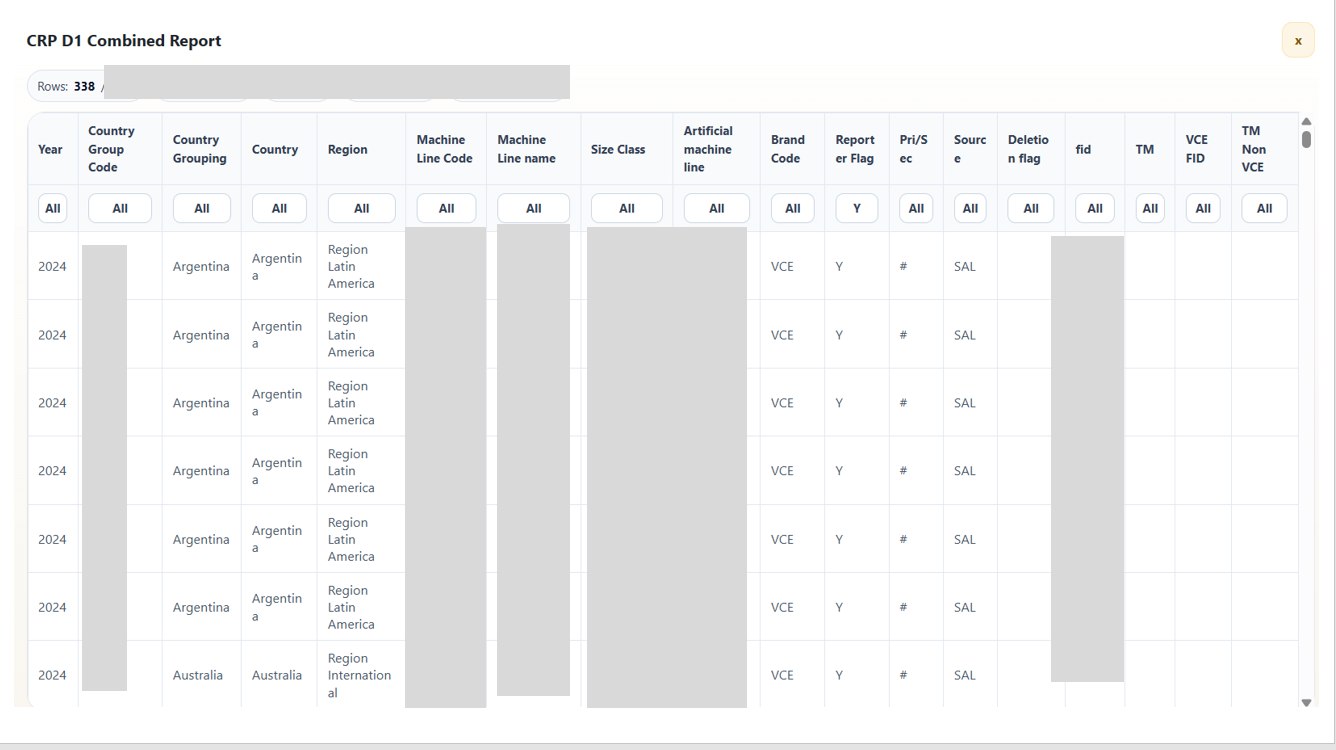
\includegraphics[width=1.1\linewidth]{6.1.png}
    \caption{CRP preparation validation result}
    \label{fig:crp_preparation_validation}
\end{figure}

\begin{figure}[H]
    \centering
    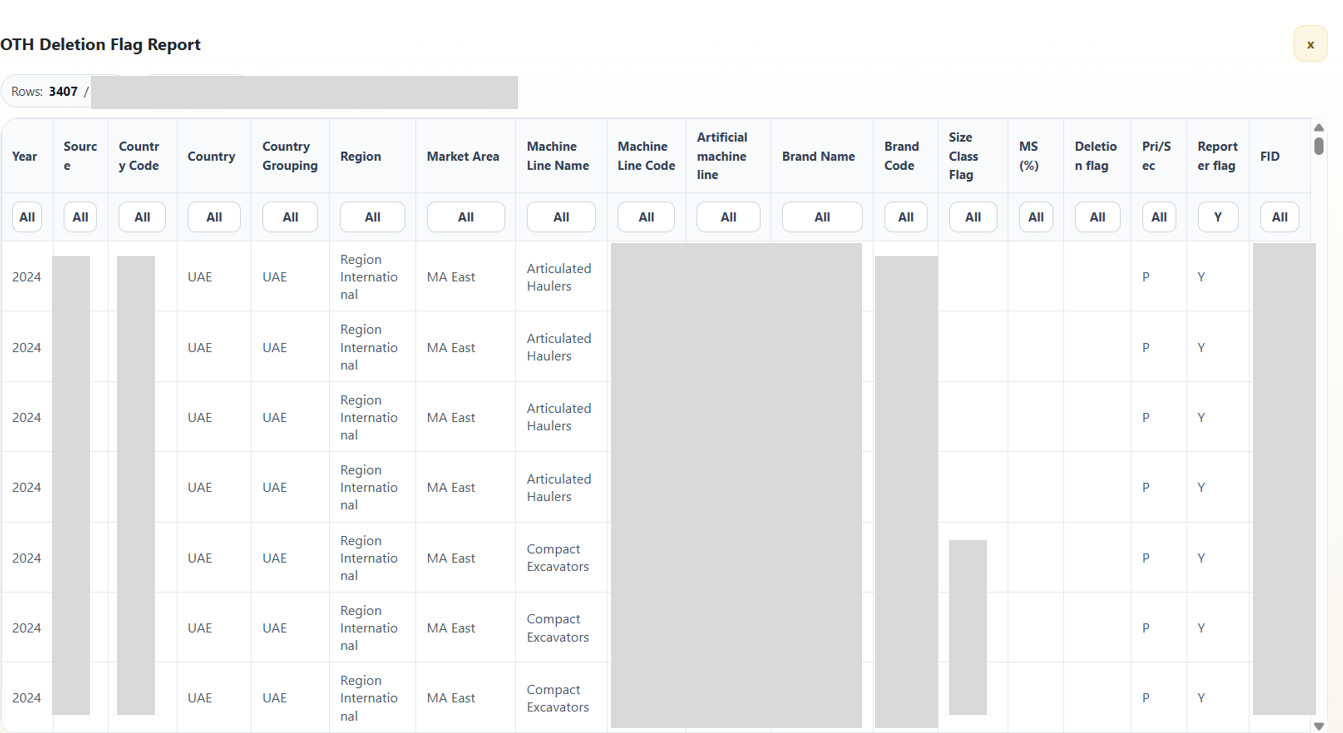
\includegraphics[width=1.1\linewidth]{6.2.png}
    \caption{OTH deletion flag and reporter flag validation result}
    \label{fig:oth_deletion_report_validation}
\end{figure}



\subsection{Split- and Resplit-Related Validation}

The split- and resplit-related outputs were validated through manual Excel-based checks, SAP reference comparison, and output inspection. For split validation, records that should enter the split process were manually filtered in Excel and compared with the prototype's split input totals. The totals were consistent for the tested Excavators and Wheel Loaders split cases, indicating correct record selection.

Approximately 10\% of split output rows and 10\% of resplit output rows were then spot-checked across selected country, source, machine-line, and size-class combinations. The sampled records followed the intended split and resplit logic, and the before/after totals remained consistent. Some differences from SAP outputs were nevertheless observed. Part of that difference was again related to reporter-list version differences, while one reviewed case suggested a different split-ratio basis in SAP than in the prototype. These findings were treated as reference-data and rule-clarification issues rather than direct prototype failures. Overall, the split and resplit logic behaved correctly within the tested scope.

\begin{figure}[H]
    \centering
    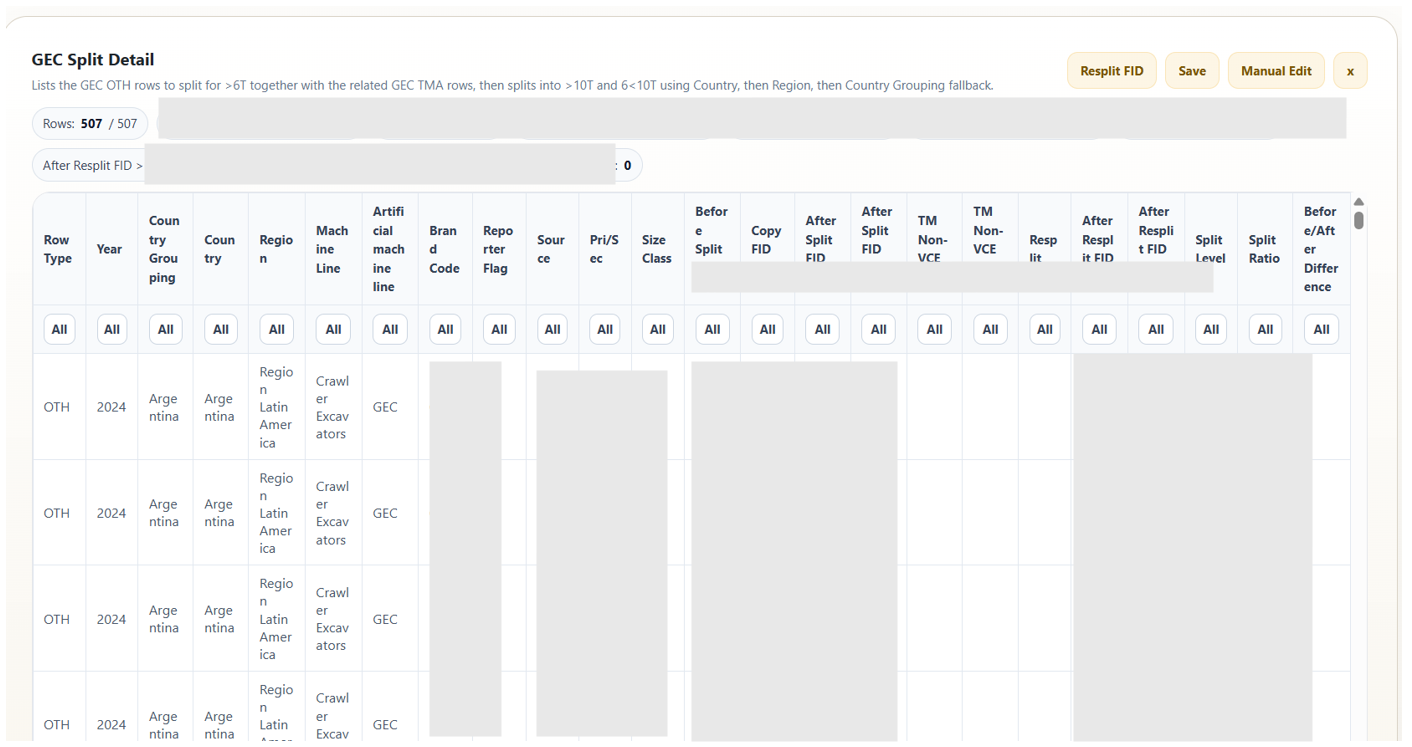
\includegraphics[width=1.1\linewidth]{6.3.png}
    \caption{Example of split and resplit validation results for GEC records}
    \label{fig:gec_split_resplit_validation}
\end{figure}

% \subsection{Summary of Validation Evidence and Results}

% Table~\ref{tab:data_evidence_validation} summarises the main validation evidence and results from the tested 2024 workflow data.

% \begin{longtable}{|>{\raggedright\arraybackslash}p{3.6cm}|>{\raggedright\arraybackslash}p{4.1cm}|>{\raggedright\arraybackslash}p{6.2cm}|}
% \caption{Summary of validation evidence and results}
% \label{tab:data_evidence_validation} \\
% \hline
% \textbf{Validation Area} & \textbf{Evidence / Data Checked} & \textbf{Validation Result} \\
% \hline
% \endfirsthead

% \hline
% \textbf{Validation Area} & \textbf{Evidence / Data Checked} & \textbf{Validation Result} \\
% \hline
% \endhead

% Preparation control flags & CRP reporter rows: 338; OTH reporter-flag rows: 3,407. & Reporter-related preparation outputs matched the expected classifications and corresponding SAP reference results. \\
% \hline

% Mapped fields & Country, market area, and related mapped fields checked against SAP export tables. & The mapped fields were aligned with the SAP-generated values in the tested 2024 data. \\
% \hline

% Market-view calculation & Approximately 20\% of rows sampled across selected country and machine-line combinations. & The sampled records showed correct TMA reduction by Volvo CE sales and correct VCE / Non-VCE ratio calculation. \\
% \hline

% Split and resplit outputs & Split-row selection and approximately 20\% of split/resplit rows sampled. & Split levels, split ratios, redistributed values, and before/after totals were consistent with expected rules in the sampled cases. \\
% \hline

% Runtime observation & Demonstration runs across preparation, market-view, adjustment, and split/resplit stages. & The prototype completed the tested runs within practical review time for prototype-level evaluation. \\
% \hline

% Stability observation & Repeated upload, run, filter, save/reload, and export cycles. & No crash, data loss, or inconsistent save/reload behaviour was observed in the tested scope. \\
% \hline

% \end{longtable}

% \section{Evaluation Against Requirements}

% The artefact was further evaluated against the requirements defined in Section~\ref{sec:requirements}. Each requirement was linked to an evaluation parameter and assessed using prototype functions, generated outputs, validation checks, runtime/stability observations, and stakeholder feedback.

% SAP reference outputs were used where direct comparison was possible, mainly for preparation-, split-, and resplit-related validation. Transparency, traceability, and usability were evaluated through prototype functions, visible intermediate outputs, available source/rule context fields, and stakeholder feedback. Performance and stability were assessed through observed execution and repeated review operations.

% The results are summarised in Table~\ref{tab:evaluation_parameters}.

% \begin{longtable}{|>{\raggedright\arraybackslash}p{1.2cm}|>{\raggedright\arraybackslash}p{2.7cm}|>{\raggedright\arraybackslash}p{4.0cm}|>{\raggedright\arraybackslash}p{6.0cm}|}
% \caption{Evaluation against requirements}
% \label{tab:evaluation_parameters} \\
% \hline
% \textbf{ID} & \textbf{Evaluation Dimension} & \textbf{Evaluation Parameter} & \textbf{Evaluation Result} \\
% \hline
% \endfirsthead

% \hline
% \textbf{ID} & \textbf{Evaluation Dimension} & \textbf{Evaluation Parameter} & \textbf{Evaluation Result} \\
% \hline
% \endhead

% FR1 & Functional fulfilment & Completion of source and matrix file upload and management. & Source and matrix files were uploaded, stored, displayed, downloaded, and reused across downstream stages. \\
% \hline

% FR2 & Functional fulfilment & Successful execution of backend workflow processing. & Backend processing executed preparation, adjustment, and split/resplit logic and produced outputs used for rule and SAP-reference validation. \\
% \hline

% FR3 & Functional fulfilment / usability & Availability of frontend review functions. & Filterable tables, summaries, charts, and CSV export supported browser-based review of detailed and aggregated outputs. \\
% \hline

% SR1 & Structural fit & Separation of upload, processing, storage, and visualisation components. & The artefact used a modular frontend-backend-database architecture with separated responsibilities. \\
% \hline

% SR2 & Structural fit & Structured storage of uploaded files, mappings, workflow records, and generated outputs. & Structured persistence supported repeated review, save/reload behaviour, and extension to later workflow stages. \\
% \hline

% PR1 & Performance & Successful completion of stage and report execution for the selected 2024 dataset. & Demonstration runs completed successfully across preparation, market-view, adjustment, and split/resplit flows. Observed execution time was typically within a few seconds and up to around one minute depending on stage complexity and row volume; formal production benchmarking was outside the thesis scope. \\
% \hline

% PR2 & Performance / stability & Absence of crashes, data loss, or inconsistent save/reload behaviour during repeated operations. & Repeated upload, run, filter, save/reload, and export cycles were executed during demonstration and validation. No crash, data-loss event, or inconsistent save/reload behaviour was observed in the tested 2024 scope. \\
% \hline

% QR1 & Transparency & Visibility of intermediate workflow stages, row-level outputs, and stage summaries. & Stage-specific views and outputs, including OTH deletion base, preparation, adjustment, and split/resplit, allowed stepwise inspection of how values were formed from one stage to the next. \\
% \hline

% QR2 & Traceability & Availability of source, mapping, control-flag, and rule-decision context in generated stage outputs. & Generated tables included source, country, machine line, artificial machine line, brand, reporter/deletion flags, split level, and split ratio fields, enabling stage-level traceability between uploaded inputs, applied rules, and resulting outputs. \\
% \hline

% QR3 & Usability & Ability to complete BI review tasks through the browser interface with acceptable effort. & Users completed review tasks through browser navigation, table filtering, summary/chart inspection, and CSV export. Stakeholder feedback indicated that these functions improved practical review compared with the prior representation. \\
% \hline

% ER1 & Environmental fit & Operation in a controlled prototype environment. & The artefact ran as a browser-accessible prototype with web frontend, backend service, and relational database for demonstration and evaluation. \\
% \hline

% ER2 & Environmental fit & Future adaptability to more robust cloud or Volvo CE internal infrastructure. & The modular design supports future adaptation to cloud or Volvo CE internal infrastructure; full enterprise integration remains future work. \\
% \hline

% \end{longtable}











% \section{Evaluation Against Requirements}

% The artefact was evaluated against the requirements defined in Section~\ref{sec:requirements}. Each requirement was assessed through generated outputs, SAP reference comparisons where applicable, runtime observations, repeated stability testing, and stakeholder feedback. Five repeated workflow runs with the selected 2024 dataset were used to record execution times for the main workflow stages.

% Stakeholder feedback was collected during prototype demonstrations and review discussions with Business Intelligence-related stakeholders in Volvo CE Strategy and Business Development, focusing on whether the separated workflow views, filters, summaries, and intermediate outputs made the selected TMC stages easier to inspect, validate, and discuss than in the SAP-based representation.

% The results are summarised in Table~\ref{tab:evaluation_parameters}.

% \begin{longtable}{|>{\raggedright\arraybackslash}p{3.2cm}|>{\raggedright\arraybackslash}p{4.6cm}|>{\raggedright\arraybackslash}p{6.2cm}|}
% \caption{Evaluation against requirements}
% \label{tab:evaluation_parameters} \\
% \hline
% \textbf{Requirement} & \textbf{Evaluation Question / Metric} & \textbf{Evidence and Result} \\
% \hline
% \endfirsthead

% \hline
% \textbf{Requirement} & \textbf{Evaluation Question / Metric} & \textbf{Evidence and Result} \\
% \hline
% \endhead

% FR1 Functional fulfilment & Can required source and matrix files be uploaded, shown, downloaded, and reused? & Yes. The required datasets in scope were uploaded and reused in workflow execution, including Source Matrix, Reporter List, Size Class, Brand Mapping, Group Country, Machine Line Mapping, OTH, CRP- and TMA-related data, and Volvo CE sales data. Upload pages supported \textit{Show Latest} and \textit{Download Latest}. \\
% \hline

% FR2 Functional fulfilment & Can backend logic generate staged workflow outputs? & Yes. The backend generated OTH deletion and reporter base outputs, preparation outputs, market-view outputs, adjustment outputs, and split/resplit outputs used in later validation. \\
% \hline

% FR3 Functional fulfilment / usability & Can users inspect outputs through frontend review functions? & Yes. Users reviewed outputs through filterable tables, summary cards, chart-based views, and CSV export. These functions were used in demonstration and validation tasks. \\
% \hline

% SR1 Structural fit & Are upload, processing, storage, and visualisation modularised? & Yes. The prototype operated with separated frontend pages, backend report and processing routes, and relational storage for uploaded and derived records. \\
% \hline

% SR2 Structural fit & Is workflow data persisted in structured form for repeated review? & Yes. Uploaded files, mapping data, intermediate records, and generated outputs were persisted and reused across stages, including repeated save/reload review cycles. \\
% \hline

% PR1 Performance & Can the 2024 workflow be completed within the defined 40-minute review window? & The selected 2024 workflow was tested \textbf{five} times and completed within the defined \textbf{40-minute} review window. The observed time ranges were approximately \textbf{4--5 minutes} for \textit{Upload Submit Matrix}, \textbf{5--6 minutes} for \textit{Upload OTH Data} and \textit{Upload CRP Data}, \textbf{10 minutes} for the preparation stage, \textbf{3 minutes} for the adjustment layer, and \textbf{10--12 minutes} for the machine line split layer. The workflow completion time included processing, result inspection, manual correction, and saving. \\
% \hline

% PR2 Performance / stability & Is behaviour stable during repeated upload, run, filter, save, reload, and export cycles? & The stability requirement was met during repeated validation runs. The prototype was tested through \textbf{five} repeated operation cycles using the selected 2024 dataset. Each cycle covered matrix upload, OTH/CRP upload, preparation, adjustment, machine line split, filtering, manual correction, saving, reload, and CSV export. The average completion time for a full workflow cycle was approximately \textbf{33 minutes}, remaining within the defined 40-minute review window. No crash, data loss, or inconsistent save/reload behaviour was observed. \\
% \hline

% QR1 Transparency & Are intermediate stages directly inspectable? & Yes. Stage outputs were visible separately, including OTH deletion base, preparation, adjustment, market view, and split/resplit, with row-level tables and summaries for stepwise inspection. \\
% \hline

% QR2 Traceability & Can output rows be related to source and rule context at stage level? & Partly. Outputs retained key context fields, including source, country, machine line, artificial machine line, brand, reporter/deletion flags, split level, and split ratio. This enabled stage-level tracing. Full end-to-end row lineage remains future work. \\
% \hline

% QR3 Usability & Can BI users complete review, validation, and export tasks with acceptable effort? & Yes within the prototype scope. Stakeholders could navigate stages, apply filters, inspect summaries/charts, and export CSV. Review feedback indicated improved practical inspectability compared with the prior representation. \\
% \hline

% QR4 Validation support & Do outputs match SAP and business-rule expectations where comparison is possible? & 
% Mostly yes.
% \begin{itemize}[leftmargin=*]
%     \item Manual Excel checks confirmed that the prototype applied the predefined rules correctly before comparison with SAP reference data. CRP reporter rows matched the SAP result, with 338 rows identified.
%     \item For OTH, the prototype classified 3,452 reporter rows, while SAP contained 3,467 rows with a net FID difference of 68. This was traced to a reporter-list version difference rather than a prototype error.
%     \item About 20\% of market-view rows and 10\% of split/resplit rows were spot-checked. The sampled records were consistent with expected calculations, split-case selection, redistribution logic, and before/after total preservation. One split-ratio discrepancy was recorded as a rule-clarification finding.
% \end{itemize}
% \\
% \hline

% ER1 Environmental fit & Can the artefact run in a controlled prototype environment? & Yes. The system was evaluated as a browser-accessible prototype with frontend, backend service, and relational database using 2024 workflow data. \\
% \hline

% ER2 Environmental fit & Is future adaptation to cloud or internal infrastructure feasible? & Partly. The modular design supports adaptation to cloud or Volvo CE internal infrastructure, but enterprise integration, production deployment, and internal authentication/integration constraints remain future work. \\
% \hline

% \end{longtable}




\subsection{Evaluation Against Requirements}

The artefact was evaluated against the functional and performance requirements defined in Section~\ref{sec:requirements}. The assessment combined generated workflow outputs, SAP reference comparisons where applicable, manual Excel checks, runtime observations, repeated stability testing, and stakeholder feedback from weekly review discussions.

Overall, the results indicate that the main requirements were met within the prototype scope. The system supported upload and reuse of the required datasets, generated staged outputs for the selected workflow layers, and provided structured inspection through filters, summaries, charts, and CSV export. Validation support was also largely confirmed: manually checked rule behaviour matched the prototype outputs, CRP reporter rows matched the SAP reference result, and sampled market-view and split/resplit records followed the expected calculation logic. The main observed exception was an OTH reporter-row difference that was traced to a reporter-list version difference rather than a prototype error.

Performance and stability results were also acceptable for the evaluated setting. Repeated workflow cycles remained within the defined review window, and no crash, data loss, or inconsistent save/reload behaviour was observed during the repeated test runs. A more detailed requirement-by-requirement table is provided in Appendix~\ref{app:supplementary-material}.








% \section{Comparison with the SAP-Based Workflow}

% To further clarify transparency, traceability, usability, and validation support, the prototype was compared with the SAP-based workflow from a business-user perspective. The comparison does not claim that SAP lacks these capabilities technically, but assesses whether they are directly available and inspectable for business users within the reviewed workflow.

% \begin{longtable}{|>{\raggedright\arraybackslash}p{2.8cm}|>{\raggedright\arraybackslash}p{2.5cm}|>{\raggedright\arraybackslash}p{2.5cm}|>{\raggedright\arraybackslash}p{5.8cm}|}
% \caption{Concise comparison between SAP-based representation and prototype}
% \label{tab:sap_prototype_comparison} \\
% \hline
% \textbf{Dimension} & \textbf{SAP-based Workflow} & \textbf{Prototype} & \textbf{Evidence in this thesis} \\
% \hline
% \endfirsthead

% \hline
% \textbf{Dimension} & \textbf{SAP-based Workflow} & \textbf{Prototype} & \textbf{Evidence in this thesis} \\
% \hline
% \endhead

% Transparency & Limited for business-user inspection & Supported & Preparation, adjustment, and split/resplit are exposed as separate inspectable stages with row-level and summary views. \\
% \hline

% Traceability & Limited and dispersed across technical structures & Partly supported & Stage outputs preserve source/rule context fields, including country, machine line, source, brand, flags, split level, and split ratio, enabling stage-level tracing. \\
% \hline

% Usability & Requires more SAP-specific navigation & Supported & Browser-based filtering, summaries/charts, and CSV export supported practical BI review tasks. \\
% \hline

% Validation support & Often requires extra extraction or IT support & Supported & Intermediate values, totals, and split parameters were directly inspectable and comparable with expected rules and SAP references. \\
% \hline

% \end{longtable}



\section{Comparison with the SAP-Based Workflow}

To further clarify transparency, traceability, usability, and validation support, the prototype was compared with the SAP-based workflow from a business-user perspective. The comparison does not claim that SAP lacks these capabilities technically, but assesses whether they are directly available and inspectable for business users within the reviewed workflow.

Compared with the SAP-based representation, the prototype made four differences visible within the evaluated scope. First, transparency improved because preparation, adjustment, and split/resplit outputs were exposed as separate inspectable stages rather than being dispersed across technical SAP artefacts. Second, traceability improved at stage level because outputs retained source and rule context such as country, machine line, source, brand, flags, split level, and split ratio. Third, usability improved because business users could review results through browser-based filtering, summaries, charts, and CSV export rather than SAP-specific navigation. Fourth, validation became more direct because intermediate values and rule-relevant fields could be inspected without additional extraction or IT-supported investigation.








% \section{Summary and Limitations}

% The evaluation showed that the artefact fulfilled its core purpose as a web-based prototype for the selected TMC workflow stages. Within the implemented scope, it supported structured CSV upload, staged backend processing, workflow-layer inspection, and validation against 2024 SAP reference results and expected business rules. It also supported transparency, stage-level traceability, usability, validation support, and prototype-level performance in the controlled test setting.

% Several limitations nonetheless apply:
% \begin{itemize}
% \item The prototype covers only selected stages of the broader TMC process, and the formal evaluation scope was limited to outputs up to machine line split/resplit.
% \item The validation was conducted with data from the 2024 calculation cycle, so the results cannot yet be generalised across all years and workflow variations.
% \item The artefact supports stage-level traceability, but full row-level lineage across all transformations remains future work.
% \item The artefact remains sensitive to the structural quality of uploaded CSV files and mapping data, despite the cleaning and normalisation logic that has been implemented.
% \item The current deployment and storage setup is adequate for prototype use, but broader internal deployment would require more robust infrastructure and deeper integration with enterprise systems.
% \end{itemize}

\section{Summary and Limitations}

The evaluation showed that the artefact fulfilled its core purpose as a web-based prototype for the selected TMC workflow stages. Within the implemented scope, it supported structured CSV upload, staged backend processing, intermediate output inspection, and rule-based validation against 2024 SAP reference outputs where comparison was possible. The results indicate that the prototype improved transparency and stage-level traceability by making preparation, market-view, adjustment, and split/resplit outputs easier to inspect and verify.

The validation results were largely consistent with the expected business rules. CRP preparation matched the SAP reference output, while the observed OTH reporter-flag difference was traced to a reporter-list version difference rather than a prototype error. For split and resplit, Excel-based checks showed that totals were preserved and sampled records followed the expected split-case, redistribution, and size-class flag rules. One split-ratio difference was identified as a rule-clarification issue.

Several limitations nonetheless apply:
\begin{itemize}
    \item The prototype covers only selected stages of the broader TMC process. Formal evaluation was limited to source upload, preparation, market-view derivation, adjustment, and selected split/resplit-related outputs.
    \item The validation was based on the 2024 calculation cycle, so the findings cannot yet be generalised to all years, source configurations, or annual workflow variations.
    \item Some SAP comparisons were affected by reference-data or calculation-basis differences, such as the reporter-list adjustment and the observed split-ratio discrepancy.
    \item The artefact supports stage-level traceability, but full row-level lineage across all transformations remains future work.
    \item The current deployment and storage setup is adequate for prototype demonstration, but broader internal use would require more robust infrastructure, access control, and integration with enterprise systems.
\end{itemize}


% !TEX root = ../Thesis.tex

\chapter{Conclusions and Discussion} 
\label{cha:Discussion}


% \section{Reflection on the Artefact Development}


\section{Answer to the Research Questions}







\subsection{Answer to Sub-RQ1: How can the architecture and data handling of a web-based prototype be designed to support structured upload, storage, and management of heterogeneous workflow inputs, including source datasets and matrix-based business rules?}


Sub-RQ1 is addressed by implementing a web-based input management layer that supports structured upload, review, and versioning of workflow files. The prototype provides dedicated upload interfaces for both source datasets and matrix inputs. Uploaded files are validated, normalised, and stored together with metadata such as file type, timestamp, processing status, row count, and version information. This makes it possible to track which input files were used and to retrieve the latest valid version of each required dataset.

The frontend also supports practical management actions such as viewing uploaded data, downloading stored inputs, and saving edited data as a new version. In this way, input handling becomes a traceable process rather than a one-time file upload. Users can inspect rows directly in the interface and verify whether required inputs are available before running downstream workflow steps.

The 2024 evaluation showed that different source and matrix files could be ingested, stored, retrieved, downloaded, and re-saved correctly. Therefore, the artefact answers Sub-RQ1 by making workflow inputs easier to access, manage, inspect, and reuse through a structured web-based interface.



% \subsection{Answer to Sub-RQ2: How can the preparation, adjustment, and machine line split stages of the TMC workflow be re-expressed in a web-based environment so that intermediate transformations and derived results become inspectable and traceable for business users?}


% Sub-RQ2 is addressed by re-expressing the preparation, adjustment, and machine line split stages as explicit web-based workflow layers with persisted intermediate outputs, rule-visible fields, and stage-specific inspection views.

% \begin{itemize}
%     \item \textbf{Preparation re-expression:}  
%     Preparation is implemented as a dedicated processing layer that validates, cleans, and aligns CRP, SAL, and OTH with matrix-based rules (source, country grouping, machine line, brand, and size class). The system exposes mapped dimensions and control fields (e.g., reporter and deletion-related flags), making the interpretation of raw rows inspectable before downstream calculations.

%     \item \textbf{Adjustment re-expression:}  
%     Adjustment is represented as a separate regrouping layer that outputs both source-detail and derived rows in a common review structure. This makes the transformation from prepared data to adjusted results traceable at row level and aggregate level.

%     \item \textbf{Machine line split re-expression:}  
%     Split is represented as an explicit redistribution layer where grouped OTH values are transformed into finer machine-line and size-class buckets using rule-based split ratios derived from prepared references. Before/after values and split details are exposed so users can verify redistribution logic directly.

%     \item \textbf{Traceability and inspection mechanism:}  
%     Workflow execution is presented through Pipeline Viewer (stage status, readiness, dependencies) and Layer Detail pages (row-level outputs, summaries, rule-related fields). Together, these views connect stage-level monitoring with record-level validation and make intermediate transformations and derived results traceable across the full workflow path.
% \end{itemize}

% This layered web representation turns previously embedded transformations into explicit, inspectable, and traceable workflow stages for business users.


\subsection{Answer to Sub-RQ2: How can staged data-processing activities be re-expressed in a web-based environment so that intermediate transformations and derived results become inspectable and traceable for business users?}

Sub-RQ2 is answered by representing selected workflow stages as explicit web-based layers with persisted intermediate outputs and stage-specific inspection views. In the case setting, this covers preparation, adjustment, and machine line split. Preparation validates, cleans, and aligns CRP, SAL, and OTH data with matrix-based rules while exposing mapped dimensions and control fields. Adjustment is represented as a separate reviewable step that keeps source-detail and derived rows visible in a common structure. Machine line split makes redistribution logic explicit by exposing split ratios, before/after totals, and redistributed rows. Pipeline Viewer and Layer Detail pages then connect workflow-level monitoring with record-level inspection. Together, these design choices turn selected SAP-embedded transformations into explicit, inspectable, and traceable workflow stages.



% \subsection{Answer to Sub-RQ3: To what extent does the implemented prototype improve transparency, usability, and traceability in the TMC workflow compared to the existing SAP-based representation, as assessed through demonstration and stakeholder feedback?}


% In the SAP-based representation, the TMC workflow is organized as technical calculation steps, but intermediate logic is distributed across multiple system objects (e.g., matrix structures, planning functions/sequences, and reporting objects), which makes business-side inspection and step-by-step validation difficult. In practice, users can run the process, but tracing how a specific output is formed from CRP, SAL, OTH, and matrix rules is less direct.

% In the implemented prototype, the same workflow is exposed through explicit web-based inspection flows. Input handling is centralized through matrix/upload pages with latest-version retrieval, download, and edited-save operations; workflow-state visibility is provided through Pipeline Viewer; and stage-level result inspection is provided through Layer Detail pages with row-level outputs, summaries, and rule-related fields. This structure makes preparation, adjustment, and split transformations directly visible and easier to audit.

% Compared with the SAP-based representation, the prototype improved transparency, usability, and traceability in the evaluated scope. Demonstration with 2024 workflow data showed outputs consistent with manually verified reference results in the tested cases, and stakeholder feedback indicated clearer understanding of intermediate steps and easier validation of derived results.

% The improvement was assessed through demonstration with 2024 workflow data and stakeholder feedback. The evaluation showed that, within the implemented scope, the prototype met the main expectations by making intermediate workflow stages more visible, results easier to inspect, and validation more practical. Compared with the existing representation, users could follow dependencies and transformations more directly through the web-based views, which reduced ambiguity and increased confidence during result checking. Overall, stakeholders viewed the prototype as a more transparent and usable representation of the evaluated TMC stages.

\subsection{Answer to Sub-RQ3: To what extent does the implemented prototype improve transparency, usability, and traceability compared to an existing SAP-based workflow representation, as assessed through demonstration and stakeholder feedback?}

Sub-RQ3 asked to what extent the implemented prototype improves transparency, usability, and traceability compared with an existing SAP-based workflow representation.

In the SAP-based representation, the TMC workflow is organised through technical calculation steps and system objects such as matrix structures, planning functions, planning sequences, and reporting objects. Although the process can be executed in SAP, business-side inspection of intermediate logic is less direct, especially when users need to trace how outputs are formed from CRP, SAL, OTH, and matrix-based rules.

The prototype improves this representation by exposing the workflow through dedicated web-based inspection flows. Input handling is centralised through upload and matrix-management pages, workflow progress is shown through Pipeline Viewer, and intermediate results are made available through Layer Detail pages with row-level outputs, summaries, and rule-related fields. This makes preparation, adjustment, and split-related transformations easier to inspect, validate, and discuss.

The improvement was assessed through demonstration with 2024 workflow data and stakeholder feedback. Within the evaluated scope, the prototype made intermediate stages more visible, reduced ambiguity in result checking, and supported more practical validation of derived outputs. Stakeholder feedback indicated that the separated workflow views helped users follow dependencies, inspect intermediate results, and discuss rule behaviour more directly than in the SAP-based workflow.

More broadly, this suggests that inspection-oriented representations can add value in enterprise workflows where business understanding depends on seeing how staged transformations connect inputs, rules, and outputs rather than only reviewing final reported values.


% \subsection{Restatement of the Research Question}

% This thesis addressed the following research question: \textit{How can an interactive data processing and visualization prototype be designed to improve transparency, inspectability, and usability in the Volvo CE TMC workflow?} To answer this question, three sub-questions were defined:

% \begin{itemize}
%     \item  \textbf{Sub-RQ1:} How can a web-based system support the upload, management, and display of workflow input files so that different source datasets and matrix-based business input become easier to access and inspect?
%     \item \textbf{Sub-RQ2:} How can the workflow stages of preparation, adjustment, and split be represented in a web-based system so that users can more clearly follow how results are derived from CRP, SAL, OTH, and related business rules?
%     \item \textbf{Sub-RQ3:} How can interactive UI elements, such as filtering, summary calculations, chart-based displays, and layer-based views, improve usability and support validation of intermediate and derived workflow results?
% \end{itemize}

% The developed artefact provides clear answers to these questions. For the first sub-question, the prototype introduced structured upload and display of workflow input through dedicated web-based pages for source data and matrix files. For the second sub-question, the artefact represented preparation-, adjustment-, and split-related logic through staged backend processing and inspectable layer-based views. For the third sub-question, the prototype used filtering, summary values, chart-based displays, and CSV export to support more direct review and validation of workflow results.

% Taken together, the artefact shows that a web-based prototype can make selected parts of the TMC workflow more transparent, inspectable, and usable by combining structured input handling, staged result generation, and interactive frontend inspection.


% \subsection{Restatement of the Research Question}

% This thesis addressed the following research question: \textit{How can an interactive data processing and visualization prototype be designed to improve transparency, inspectability, and usability in the Volvo CE TMC workflow?} To answer this question, three sub-questions were defined:

% \begin{itemize}
%     \item \textbf{Sub-RQ1:} How can a web-based system support the upload, management, and review of workflow input files so that different source datasets and matrix-based business input become easier to access and inspect?
%     \item \textbf{Sub-RQ2:} How can the workflow stages of preparation, adjustment, and split be represented in a web-based system so that users can more clearly follow how results are derived from CRP, SAL, OTH, and related business rules?
%     \item \item \textbf{Sub-RQ3:} How can interactive UI elements, such as filtering, summary calculations, chart-based displays, and layer-based views, improve usability and support validation of intermediate and derived workflow results?
% \end{itemize}

% The developed artefact provides clear answers to these questions. For the first sub-question, the prototype introduced structured upload, display, and download of workflow input through dedicated web-based pages for source data and matrix files. For the second sub-question, the artefact represented preparation-, adjustment-, and split-related logic through staged backend processing and inspectable layer-based views. For the third sub-question, the prototype used filtering, summary values, chart-based displays, and CSV export to support more direct review and validation of workflow results.

% Taken together, the artefact shows that a web-based prototype can make selected parts of the TMC workflow more transparent, inspectable, and usable by combining structured input handling, staged result generation, and interactive frontend inspection.




























% \subsection{Design Decisions of the Artefact}

% Several design decisions influenced the development of the artefact. First, the workflow was represented in a web-based prototype rather than within SAP itself. This was done because the aim of the thesis was to improve transparency and inspectability for business users instead of extending the existing SAP environment directly.

% Second, a modular frontend-backend architecture was adopted. This allowed upload handling, workflow processing, and result visualization to be separated into distinct components, which supported both implementation and extensibility.

% Third, CSV-based input handling was chosen as the prototype interface to workflow data. This made it possible to work with realistic workflow input while remaining independent from direct SAP integration during development and evaluation.

% Finally, the workflow was represented through inspectable layers instead of only final outputs. This decision was important for making intermediate transformations visible and for supporting validation of workflow logic in a more user-oriented way.






% \subsection{Practical Value}


% The practical value of the artefact lies in its re-expression of selected parts of the SAP-based TMC workflow in a more inspectable web-based environment. In the existing process, important workflow logic is embedded in SAP-specific planning functions, planning sequences, and matrix-related structures, which makes it difficult for business users to understand how intermediate and final results are formed. The developed prototype addresses this by translating selected parts of that logic into SQL-based backend processing and presenting the resulting workflow stages through a web interface.

% A further practical contribution is that the artefact supports structured upload, staged result generation, and direct review of intermediate and derived outputs. Through layer-based views, filterable tables, summary values, charts, and CSV export, users can inspect how values are formed and review workflow results in a more direct and transparent way.


% If deployed for internal use, the artefact could also enable the Business Intelligence team to run and inspect selected workflow stages more independently, without relying entirely on Volvo IT to execute the corresponding process in SAP. In this way, the artefact provides a more transparent basis for reviewing yearly TMC results and reduces some of the effort required to interpret workflow behaviour outside the SAP environment.




% The practical value of the artefact lies in its re-expression of selected parts of the SAP-based TMC workflow in a more transparent and inspectable web-based environment. In the existing process, important workflow logic is embedded in SAP-specific planning functions and matrix structures, making it difficult for business users to trace how values are derived. The prototype addresses this by separating input handling, processing, and result inspection into explicit and reviewable steps accessible through a standard web interface.

% A key contribution is that the artefact exposes intermediate workflow stages rather than only final aggregated outputs. Through dedicated views for preparation, adjustment, and split-related results, users can inspect how values are formed step by step, compare grouped results with source rows, and validate whether the implemented logic behaves as expected. Filterable tables, summary values, charts, and CSV export further support both overview and row-level inspection within the same interface.

% The prototype also has practical value because it was validated against manually verified 2024 SAP reference data. This indicates that the artefact is not only a conceptual demonstration, but a working system that produced outputs consistent with the tested reference cases. For the Business Intelligence team, this provides a more transparent basis for reviewing TMC results, comparing outputs, and identifying mismatches in the underlying data or rule





% From an academic perspective, this thesis provides a practical example of how a complex enterprise workflow can be re-expressed in a more inspectable and user-oriented prototype environment. By applying the Design Science Research approach, the study translates a problem of limited transparency in a SAP-based process into design requirements, artefact development, and evaluation.

% The study is also relevant to research on enterprise-system usability and transparency. Prior work has shown that usability characteristics influence end-user satisfaction in ERP systems and that information transparency affects how such systems are perceived and adopted \cite{calisir2004erp}. In addition, SAP itself has been discussed as a system where usability can become a significant issue for business users \cite{wong2016sap}. Against this background, the thesis contributes a concrete case in which selected workflow logic is moved from embedded SAP-related structures into a combination of SQL-based processing and web-based visualization.

% In this way, the thesis adds practical knowledge to research on workflow transparency, inspectability, and usability in enterprise data processes, while also showing how these goals can be addressed through an implemented prototype rather than through conceptual discussion alone.



% This thesis contributes a design approach for making complex enterprise data workflows more inspectable. Rather than treating the SAP-based TMC process as a single black-box calculation, the study decomposes selected workflow stages into separate and reviewable layers. Each layer produces intermediate outputs that can be inspected, compared, exported, and validated. This staged representation is a central contribution of the artefact, because it makes the transformation process itself visible instead of only presenting final results.

% A further artefact contribution is the combination of rule-based backend processing with interactive frontend inspection. The prototype does not only automate selected parts of the TMC workflow; it also exposes how results are formed through upload management, preparation-, adjustment-, and split-related views, filtering, summary values, charts, and export functions. In this sense, the artefact differs from a conventional dashboard, where the emphasis is mainly on final indicators. Here, intermediate data states are treated as important outputs of the system and as a basis for validation.

% Methodologically, the thesis shows how Design Science Research can be used to translate a practical organizational problem into an implemented and evaluated artefact. The study connects stakeholder needs, artefact requirements, implementation decisions, and evaluation through 2024 reference-data comparison and stakeholder feedback. This provides a structured example of how transparency, inspectability, and usability concerns can be turned into concrete design features in an enterprise data workflow.


% \subsection{Practical Contributions}





% The main practical contribution of this thesis is the development of a working web-based prototype for selected stages of the Volvo CE TMC workflow. The artefact provides a more transparent and inspectable alternative to relying only on the existing SAP-based execution and review process. By re-expressing selected workflow logic in a user-oriented web environment, the prototype demonstrates how SAP-based enterprise processes can be complemented by a dedicated validation and inspection tool.

% A key contribution is that the prototype exposes intermediate workflow outputs, including preparation, adjustment, and split-related results, rather than only presenting final aggregated figures. Through filterable tables, summary values, charts, and CSV export, users can inspect how values are formed, compare outputs with source data, and validate whether the implemented logic behaves as expected.

% For the Strategy and Business Intelligence function, the prototype offers a new digital way of working with TMC-related data. It supports process transparency, independent review, and more efficient discussion of workflow logic and data-quality issues.











% \subsection{Methodological and Artefact Contributions}

% This thesis contributes a design approach for making complex enterprise data workflows more inspectable. Instead of treating the SAP-based TMC process as a single black-box calculation, the study decomposes selected workflow stages into separate layers that can be processed, inspected, exported, and validated.

% The artefact contribution lies in combining rule-based backend processing with interactive frontend inspection. Unlike a conventional dashboard that mainly presents final indicators, the prototype treats intermediate data states as important outputs of the system. This supports both technical validation and business-user understanding.

% Methodologically, the thesis shows how stakeholder needs, artefact requirements, implementation decisions, reference-data comparison, and stakeholder feedback can be connected within a Design Science Research process. It provides an example of how organizational concerns about transparency and usability can be translated into concrete design features in an enterprise data workflow.


% \subsection{Academic Contributions}

% From an academic perspective, this thesis contributes to research on enterprise-system usability and workflow transparency by providing an implementation-oriented case in an industrial setting. Prior research has shown that usability characteristics influence end-user satisfaction in ERP systems and that information transparency affects how such systems are perceived and adopted \cite{calisir2004erp}. SAP has also been discussed as a system where usability can become a significant issue for business users \cite{wong2016sap}. This thesis extends this discussion by showing how such concerns can be addressed through a concrete prototype rather than through conceptual analysis alone.

% The academic contribution is not the proposal of a new algorithm, but practical design knowledge about how embedded ERP workflow logic can be made more transparent and inspectable. The thesis demonstrates that selected SAP-related logic can be externalized into a web-based environment while preserving step-wise traceability and supporting user-oriented validation.

% In this way, the thesis adds to existing work by showing how a black-box enterprise process can be transformed into an inspectable prototype that supports both technical validation and business-user understanding.


\section{Contributions and Originality}
\subsection{Practical Contributions}

The main practical contribution of this thesis is a case-grounded demonstration of how selected parts of an SAP-based enterprise workflow can be re-expressed in a user-oriented environment for validation, inspection, and communication without replacing the underlying operational platform. The implemented prototype for selected stages of the Volvo CE Total Market Calculation (TMC) workflow serves as the concrete instantiation of that contribution.

A key contribution is the exposure of intermediate workflow outputs, including preparation, adjustment, and split-related results, instead of only final aggregated figures. Through filterable tables, summaries, charts, and CSV export, users can inspect how values are formed and compare outputs with source data. The case therefore contributes practical design knowledge on how enterprise data-processing workflows with heterogeneous inputs, embedded rules, and sequential transformations can be made more inspectable through staged output exposure and workflow-oriented review views.

\subsection{Academic Contributions}

On the academic side, this thesis contributes a concrete example of how transparency, traceability, usability, and inspectability challenges in complex enterprise data-processing workflows can be addressed through a workflow-oriented web-based artefact. While the implemented prototype is grounded in the Volvo CE TMC case, the underlying design problem is not limited to that setting. Many enterprise workflows depend on heterogeneous inputs, embedded business rules, staged transformations, and intermediate results that are difficult for business users to inspect and validate \cite{foidl2024pipeline,putrama2024heterogeneous}.

Prior research has shown that enterprise data processing is often organised as staged ETL or decision-support workflows, that ERP usability and transparency affect how such systems are experienced by end users, and that embedded technical logic is often difficult to communicate and validate from a business perspective \cite{vassiliadis2009etl,calisir2004erp,ori2024misalignment}.

Against this background, the academic contribution of this thesis is not a new algorithm, but design knowledge about how selected enterprise workflow logic can be re-expressed in a more reviewable and business-facing form. More specifically, the thesis shows how structured input handling, staged output exposure, interactive inspection, and explicit intermediate representations can support validation, communication, and error investigation in complex enterprise data-processing workflows.

Methodologically, the thesis also provides a Design Science Research example of translating a practical enterprise workflow problem into design requirements, iterative artefact development, and formative evaluation \cite{johannesson2021}. In this way, the Volvo CE case functions as the empirical setting through which a broader workflow-design problem is investigated rather than as the sole relevance of the study.

\subsection{Originality}

The originality of this thesis lies in the independent design and development of a dedicated web-based prototype that re-expresses selected SAP-embedded workflow stages as inspectable processing layers. Before this work, there was no such solution in the studied Volvo CE context. The thesis uses that case to articulate a more general design approach for inspection-oriented enterprise workflow support.

The prototype is original in its combination of structured input management, staged processing outputs, and workflow-oriented inspection views. Instead of only reviewing final aggregated outputs, users can inspect intermediate results through tables, summaries, charts, and exportable data.

The contribution is not a new algorithm, but a case-grounded design contribution that shows how embedded enterprise workflow logic can be complemented by a more transparent, traceable, and usable inspection-oriented prototype. Although the artefact was developed in the Volvo CE setting, the underlying design idea is relevant to other enterprise workflows that involve heterogeneous data sources, rule-based transformations, and limited visibility of intermediate results. In that sense, the thesis contributes beyond the single case by showing one concrete way to externalise complex workflow logic into staged, reviewable, business-facing representations.


\section{Limitations}

Although the artefact was developed and demonstrated as a working prototype, several limitations remain.

First, the evaluation was conducted in a controlled prototype setting using selected 2024 TMC workflow data. The system has not yet been tested as a regular internal tool with broader yearly data, different workflow variations, or day-to-day business use.

Second, the implemented scope covers only selected parts of the case workflow, including preparation, market-view derivation, adjustment, and selected split/resplit-related processing. Full Total Market Calculation, full Restatement, and final Reporting were not implemented as production-level stages. The prototype should therefore be understood as a partial workflow inspection and validation tool rather than a full replacement of the SAP-based process.

Third, some rule changes are still dependent on backend development. Certain mappings, workflow conditions, and calculation logic are implemented in SQL queries and Python code, so business users cannot yet configure all rules directly through the interface.

Fourth, the prototype supports stage-level traceability, but not full end-to-end row-level lineage. Key context fields are preserved in the outputs, but the system does not yet provide a complete audit trail from every output row back to the original input rows and rule applications.

Finally, the prototype has not yet been evaluated for production-level deployment or large-scale multi-user use. Broader internal use would require authentication, monitoring, backup and recovery, process orchestration, and deployment within Volvo CE's internal infrastructure.


\section{Ethical and Societal Implications}

The artefact provides a more accessible way to process and inspect selected parts of the Volvo CE TMC workflow. The main ethical considerations concern responsible handling of company-internal data and avoiding overreliance on generated outputs. Since the results still depend on uploaded data, mappings, and implemented rules, the artefact should be treated as a validation and inspection tool rather than as a guarantee of correctness \cite{goddard2012automation}. Future use should therefore keep intermediate steps and assumptions visible so that errors can be traced and reviewed rather than hidden behind final outputs \cite{martin2019ethics}.


\section{Future Work}

Future work should address both system scope and research scope. On the system side, the artefact could be extended to later workflow stages such as full Total Market Calculation, Restatement, and Reporting, so that a larger part of the workflow can be inspected in one environment. Another important step would be to move more mappings, workflow conditions, and calculation rules out of backend code and into configurable structures, which would make the system easier to maintain as rules change over time.

Further work is also needed on traceability. The current prototype exposes intermediate stages, but it does not yet provide full end-to-end row-level lineage. A useful continuation would therefore be to strengthen drill-down from final outputs to original inputs, make rule applications more explicit, and support comparison between workflow runs. This would improve the artefact not only as a review tool, but also as a support tool for investigation and explanation.

Finally, the artefact should be studied over a longer period in regular organisational use. This would make it possible to assess its effects on validation work, communication between business and IT, and user confidence in workflow outputs. It would also allow further examination of whether the same inspection-oriented design approach can be transferred to other enterprise data-processing workflows beyond the Volvo CE case. A further research step would therefore be to apply the same design approach in another organisational setting in order to distinguish more clearly between case-specific findings and more transferable design principles.



\printbibliography
\addtocontents{toc}{\bigskip}
\addcontentsline{toc}{part}{Bibliography}

\appendix
\cleardoublepage
\addtocontents{toc}{\bigskip}
\addcontentsline{toc}{part}{Appendices}
% !TEX root = ../Thesis.tex

\chapter{Supplementary Implementation and Evaluation Material}
\label{app:supplementary-material}

\section{Software Tools and the Use of AI Tools}

Several software tools were used during the development of the artefact and the writing of the thesis.

Codex was used as a supportive tool during development, mainly for exploring implementation alternatives, discussing frontend-backend interactions, and assisting with SQL, API logic, and debugging. While it helped improve efficiency, all system design decisions and final implementations were made by the author.

ChatGPT was used during the writing process to refine language, improve clarity, and adjust phrasing to a more academic style. As English is not the author's first language, it was particularly useful for improving grammar and sentence structure. However, all ideas and conclusions were developed independently.

Visual Studio Code served as the main development environment, draw.io was used for diagrams, and Overleaf was used for writing and formatting the thesis in \LaTeX. These tools supported the development and documentation process but did not influence the research direction or results.

\section{Detailed Implementation Notes}

The prototype was implemented as a full-stack web application in which frontend actions trigger backend workflow execution through API-based processing. The implementation followed an incremental structure: authentication, routing, CSV upload, database persistence, and intermediate report generation were implemented first, after which workflow-specific calculation stages were added. This made it possible to validate each part of the execution chain separately before integrating them into the full workflow.

The frontend was implemented using React, TypeScript, Vite, and React Router. Each workflow stage is represented through route-level pages that allow users to upload data, trigger processing, inspect intermediate results, and store snapshots. The frontend does not execute workflow logic directly. Instead, it acts as an orchestration and inspection layer by sending requests to the backend through a dedicated API client and rendering the structured responses returned by backend services.

\begin{figure}[H]
    \centering
    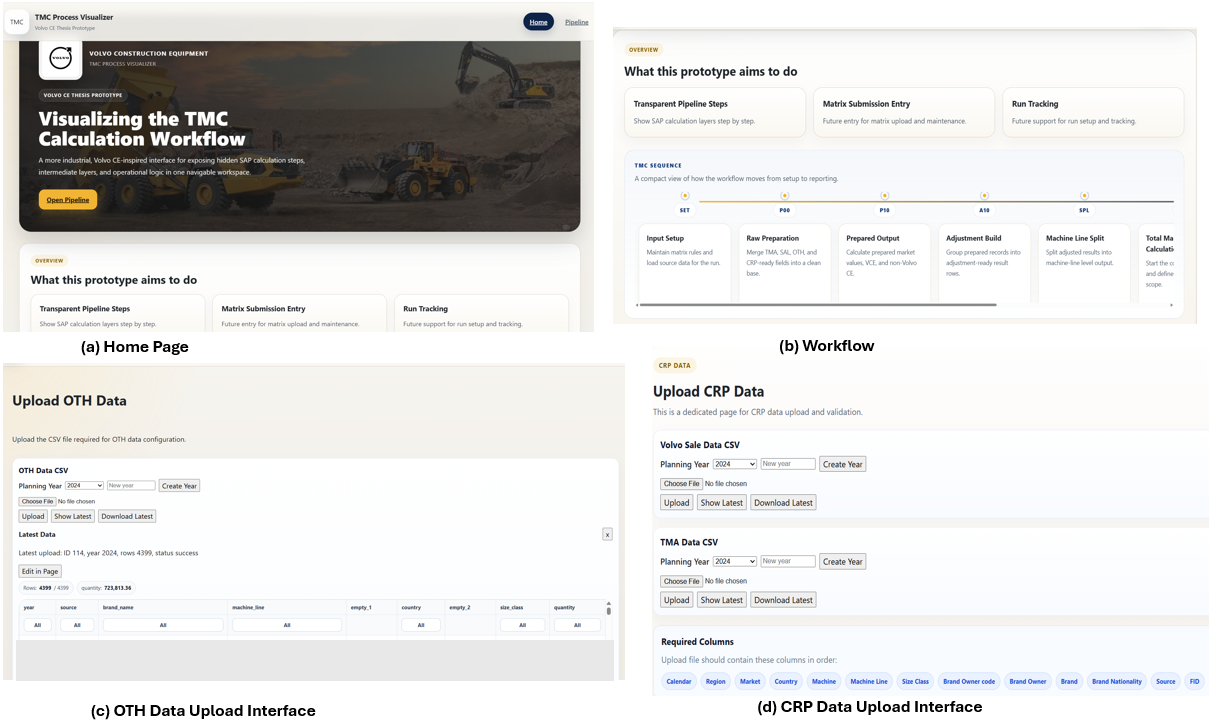
\includegraphics[width=1.1\linewidth]{5.3.1.png}
    \caption{Selected frontend views developed during the implementation of the prototype}
    \label{fig:appendix-frontend-views}
\end{figure}

The backend was implemented with Python and FastAPI. FastAPI endpoints serve as execution entry points for upload, report generation, snapshot persistence, and result retrieval. The persistence layer uses a relational database backend with environment-based switching between SQLite and PostgreSQL. During application startup, both workflow and authentication schemas are initialized before the API routes become available to the frontend.

CSV upload was implemented as the first execution stage. A user uploads a file through the frontend and selects a dataset type. The backend then routes the request to a dataset-specific handler, which parses the CSV file using \texttt{pandas}, normalizes heterogeneous input formats into a common row structure, and stores the cleaned rows in dataset-specific database tables. Upload metadata, including dataset type, planning year, upload status, and timestamp, is stored separately to support later retrieval of the latest successful input for each dataset.

Once persistence was established, source-level report generation was introduced. In this stage, backend endpoints execute SQL queries against the stored upload tables. These queries join uploaded data with mapping and control tables, such as country-group mappings, brand mappings, machine-line mappings, source matrices, and reporter lists. The purpose of these transformations is to align source data into a common workflow structure and derive control attributes such as deletion flags, reporter indicators, and primary or secondary source markers.

\begin{figure}[H]
    \centering
    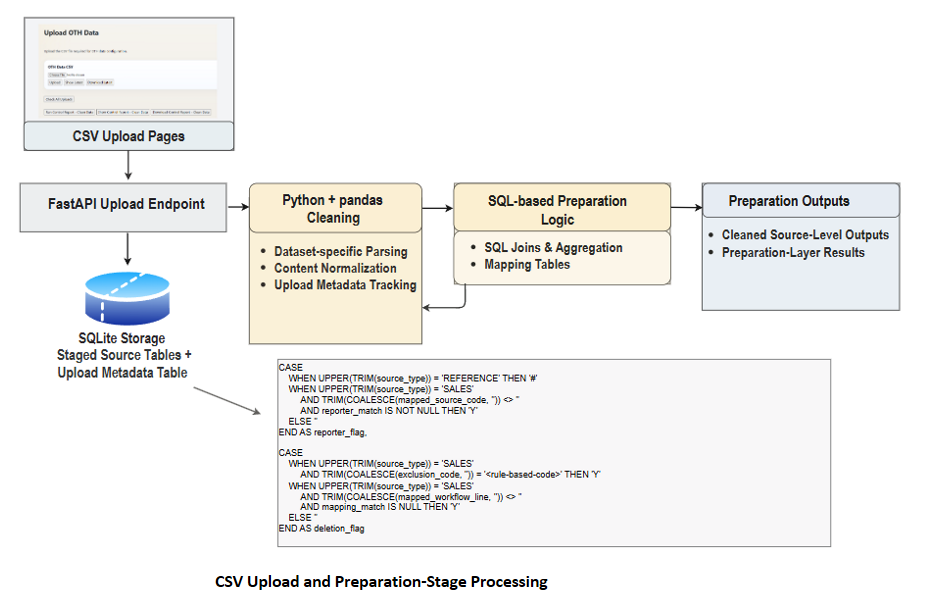
\includegraphics[width=1.1\linewidth]{5.4.png}
    \caption{Implementation of CSV upload and preparation-stage processing}
    \label{fig:appendix-upload-preparation}
\end{figure}

\begin{figure}[H]
    \centering
    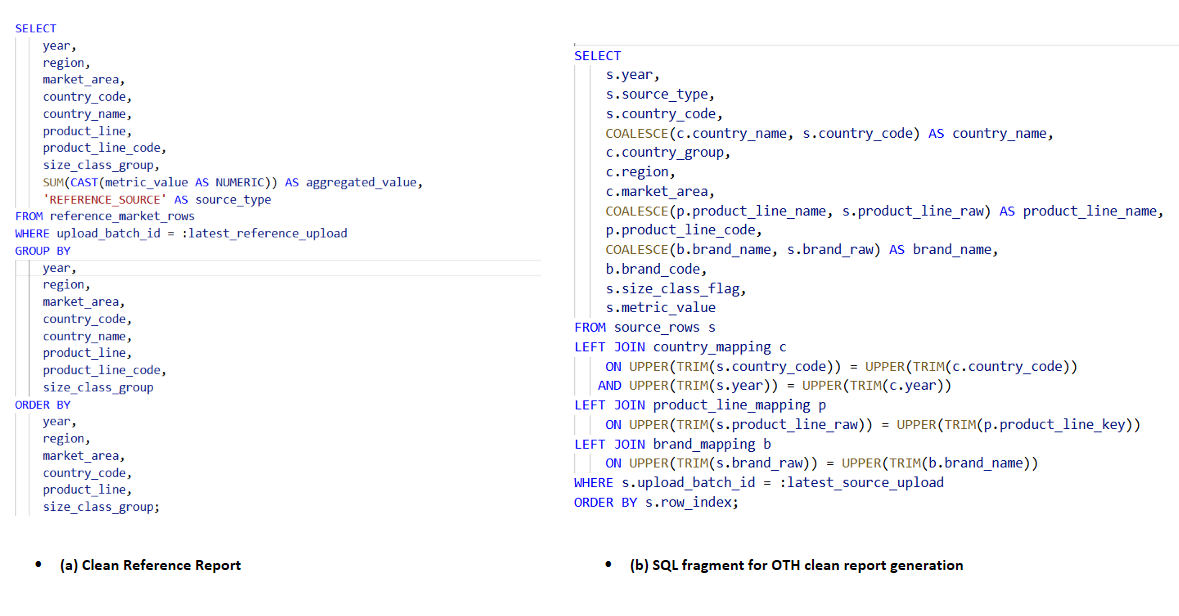
\includegraphics[width=1.1\linewidth]{5.4.1.png}
    \caption{Anonymised and simplified SQL fragments for CRP/TMA and OTH clean report generation}
    \label{fig:appendix-sql-preparation}
\end{figure}

The preparation stage follows the general execution pattern used throughout the prototype. A frontend workflow page triggers a FastAPI endpoint, which resolves the latest successful uploads, executes SQL transformations, and returns normalized rows as JSON for inspection. The same frontend-backend execution structure is reused in later workflow stages.

Adjustment-layer execution follows the same pattern, but the backend processing becomes more calculation-oriented. After the adjustment endpoint is triggered, the backend retrieves the prepared rows and executes grouped SQL queries that aggregate total-market and internal-sales values by shared workflow keys. These queries derive adjustment-layer values through conditional aggregation. The backend returns both source-detail rows and result rows, allowing the frontend to display not only the calculated output but also the data basis from which it was derived.

\begin{figure}[H]
    \centering
    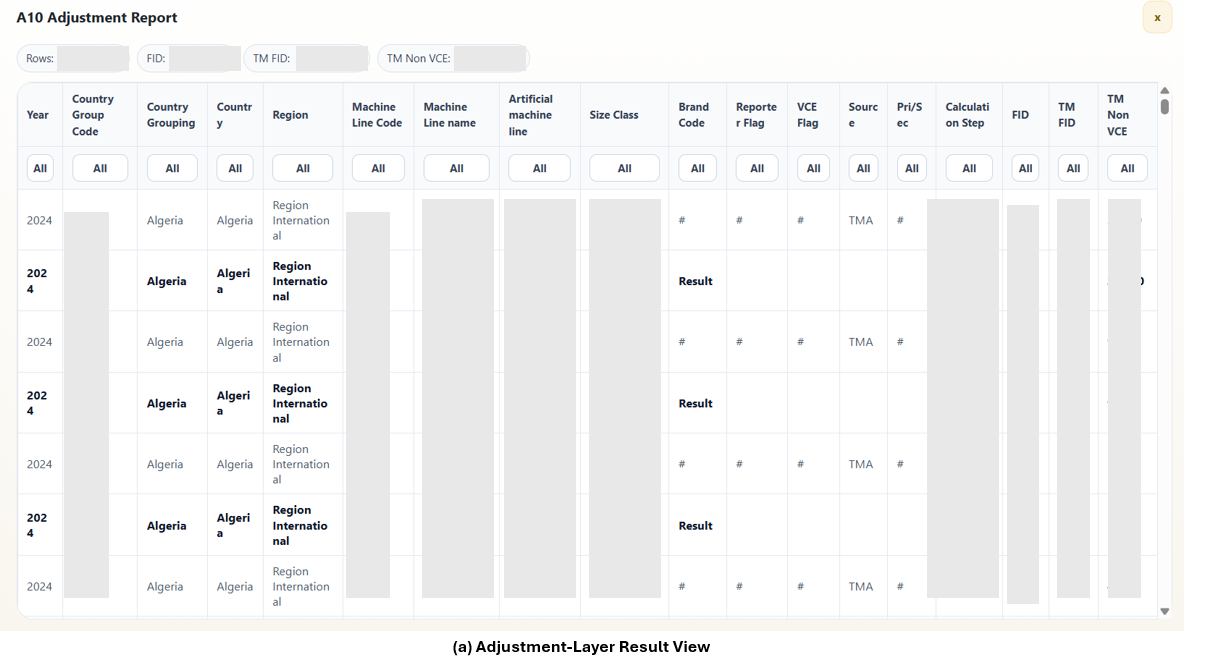
\includegraphics[width=1.1\linewidth]{5.6.1.1.png}
    \caption{Adjustment-layer result view}
    \label{fig:appendix-adjustment-view}
\end{figure}

\begin{figure}[H]
    \centering
    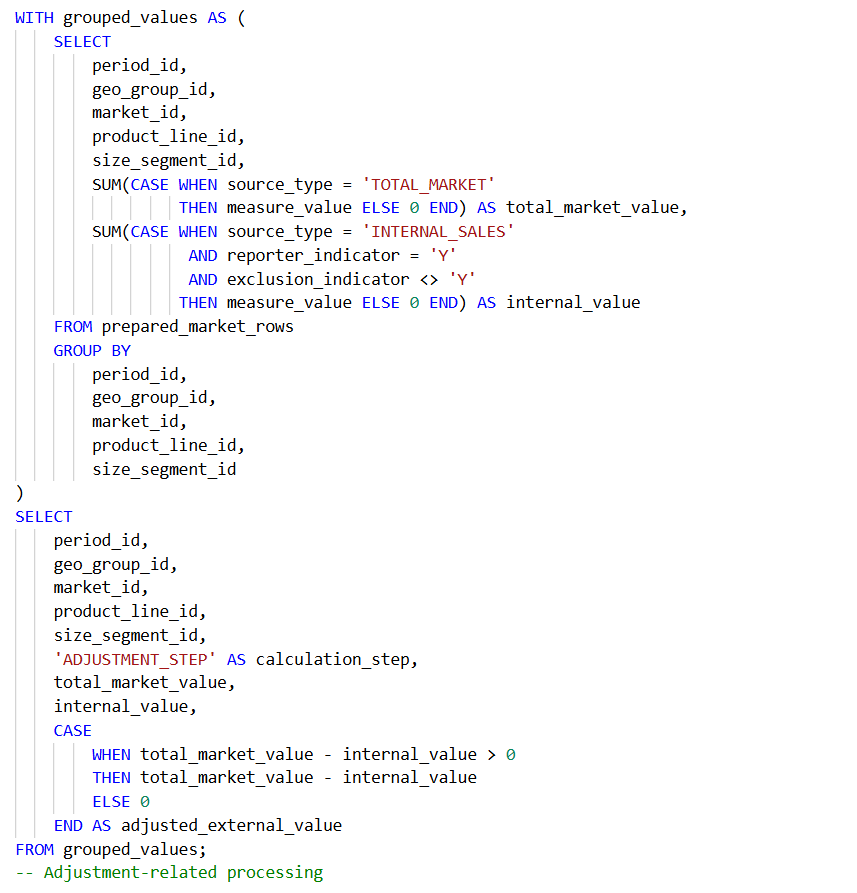
\includegraphics[width=1.1\linewidth]{5.6.1.1.1.png}
    \caption{Anonymised SQL fragment for adjustment-layer value calculation}
    \label{fig:appendix-adjustment-sql}
\end{figure}

The machine-line split stage uses a mixed execution model. SQL is used to prepare the required source and reference data, while Python is used for the redistribution calculation itself. When the user triggers a split-related report, the backend first resolves the latest required datasets and executes SQL logic to obtain eligible OTH rows and reference rows containing total-market non-VCE values. SQL therefore prepares the source rows, applies reporter and deletion logic, derives reference structures, and aggregates the values needed for proportional redistribution.

After the SQL preparation step, Python backend logic performs the split calculation. For each eligible OTH row, the backend determines the most appropriate reference level, such as country, region, or country grouping, and redistributes the input value according to the available non-VCE reference distribution. Formally, the redistribution can be expressed as:

\[
FID_{\text{split}, i}
=
FID_{\text{input}}
\times
\frac{TM_{\text{non-VCE}, i}}
{\sum_{j \in Targets} TM_{\text{non-VCE}, j}}
\]

where \(FID_{\text{input}}\) is the original OTH value to be redistributed, \(TM_{\text{non-VCE}, i}\) is the reference non-VCE value for target destination \(i\), and \(\sum_{j \in Targets} TM_{\text{non-VCE}, j}\) is the total reference non-VCE value across all valid target destinations in the same split group.

Once the calculation is completed, the backend constructs output rows containing source rows, split-result rows, supporting reference rows, split ratios, and before-after difference values. These outputs can either be saved as snapshots in the database or returned directly as JSON. The frontend then renders the results in workflow-specific inspection tables.

\begin{figure}[H]
    \centering
    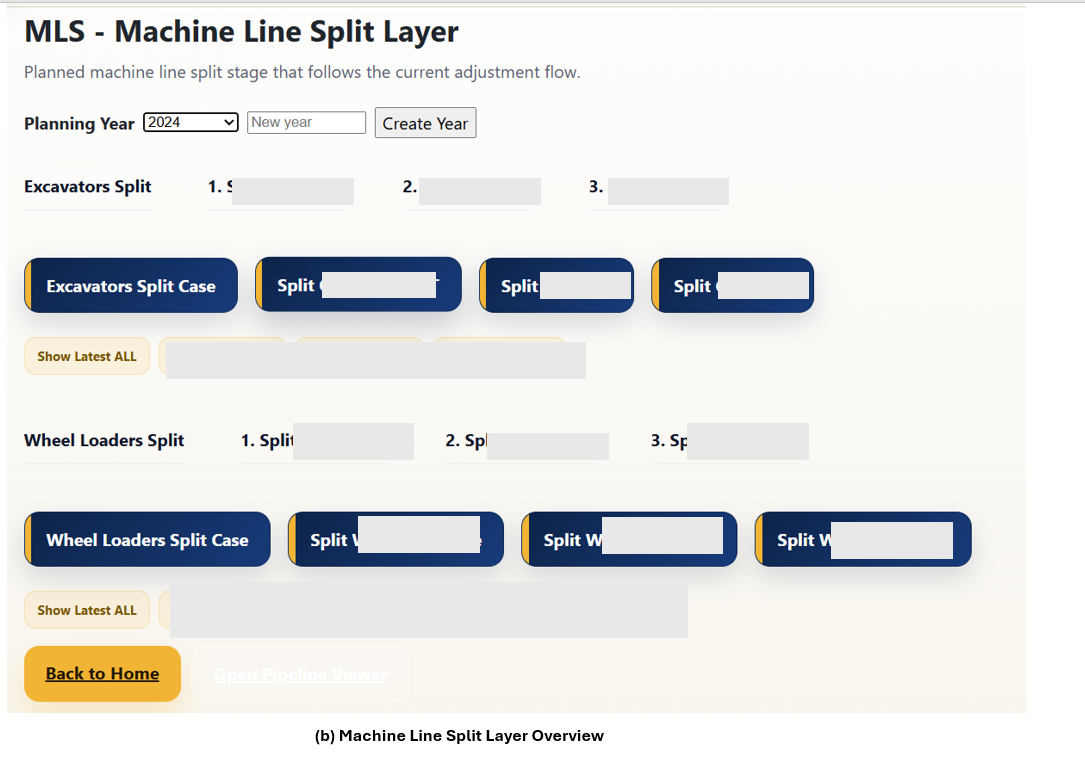
\includegraphics[width=1.1\linewidth]{5.6.1.2.png}
    \caption{Machine line split layer overview}
    \label{fig:appendix-split-overview}
\end{figure}

\begin{figure}[H]
    \centering
    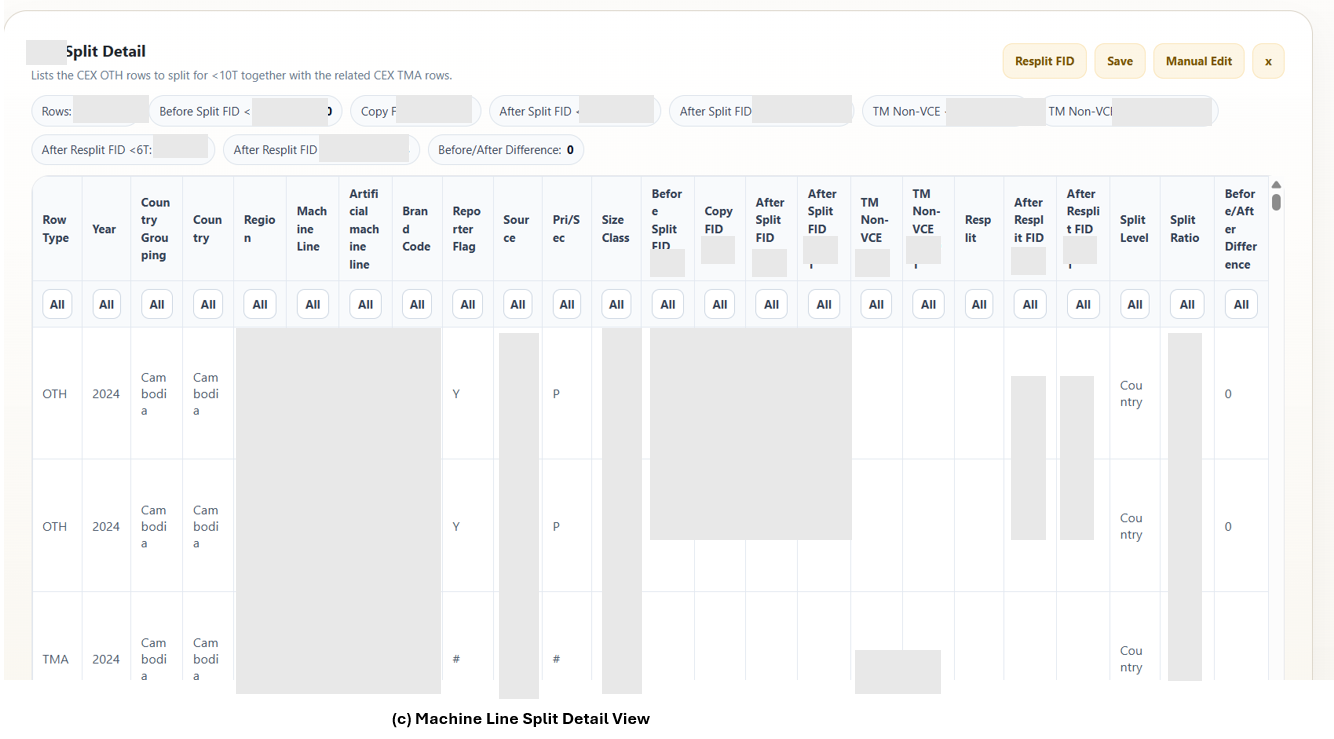
\includegraphics[width=1.1\linewidth]{5.6.1.3.png}
    \caption{Machine line split detail view}
    \label{fig:appendix-split-detail}
\end{figure}

\begin{figure}[H]
    \centering
    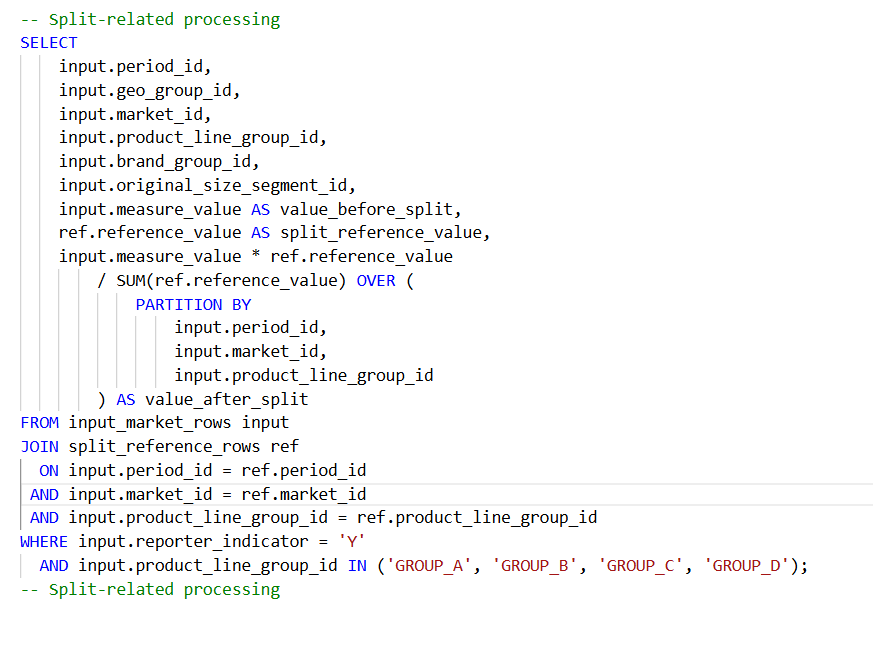
\includegraphics[width=0.85\linewidth]{5.10.png}
    \caption{Anonymised SQL and backend-processing fragments for adjustment- and split-related logic}
    \label{fig:appendix-sql-split}
\end{figure}

Frontend reporting views were developed in parallel with backend execution endpoints. They render structured JSON responses in workflow-specific inspection pages and support filtering, aggregation, and export. Overall, the implementation establishes a clear division of responsibility: the frontend triggers actions and visualizes outputs, SQL prepares and aggregates workflow data, Python handles more complex calculations such as split redistribution, and the backend returns or persists the resulting rows for later reuse.

\section{Detailed Requirement Evaluation}

The artefact was evaluated against the functional and performance requirements defined in Section~\ref{sec:requirements}. The evaluation used generated workflow outputs, SAP reference comparisons where applicable, manual Excel checks, runtime observations, repeated stability testing, and stakeholder feedback.

Stakeholder feedback was collected through weekly demo meetings and review discussions with Volvo CE stakeholders involved in the TMC workflow. During these meetings, prototype results and intermediate outputs were demonstrated, and the implemented rules were reviewed and confirmed with stakeholders. The feedback was reviewed in a qualitative and descriptive way to assess whether the separated workflow views, filters, summaries, and intermediate outputs improved practical transparency, inspectability, and usability. Manual Excel checks, output comparison, and runtime observations were used separately to assess rule correctness, validation support, and prototype performance.

\begin{longtable}{|>{\raggedright\arraybackslash}p{3.0cm}|>{\raggedright\arraybackslash}p{4.5cm}|>{\raggedright\arraybackslash}p{6.3cm}|}
\caption{Evaluation against functional and performance requirements}
\label{tab:evaluation_parameters} \\
\hline
\textbf{Requirement} & \textbf{Evaluation Question / Metric} & \textbf{Evidence and Result} \\
\hline
\endfirsthead

\hline
\textbf{Requirement} & \textbf{Evaluation Question / Metric} & \textbf{Evidence and Result} \\
\hline
\endhead

FR1 Functional fulfilment & Can required source and matrix files be uploaded, shown, downloaded, and reused? & Yes. The required datasets in scope were uploaded and reused in workflow execution, including Source Matrix, Reporter List, Size Class, Brand Mapping, Group Country, Machine Line Mapping, OTH, CRP- and TMA-related data, and Volvo CE sales data. Upload pages supported \textit{Show Latest} and \textit{Download Latest}, enabling users to review and retrieve the latest uploaded files. \\
\hline

FR2 Functional fulfilment & Can backend logic generate staged workflow outputs for the selected TMC stages? & Yes. The backend generated staged outputs for OTH deletion and reporter-base processing, preparation, market view, adjustment, and split/resplit. These outputs were used for later inspection, comparison, and validation against expected workflow logic. \\
\hline

FR3 Functional fulfilment & Does the artefact support a modular web-based frontend-backend workflow? & Yes. The prototype operated with separated frontend pages, backend report and processing routes, and relational storage for uploaded and derived records. Upload, processing, storage, workflow inspection, and visualisation were implemented as separate functions, supporting a modular workflow structure. \\
\hline

FR4 Functional fulfilment & Are uploaded files, mappings, workflow records, and generated outputs stored in a structured way for repeated review? & Yes. Uploaded files, mapping data, intermediate records, and generated outputs were stored and reused across stages. Repeated save and reload cycles confirmed that users could return to generated results and continue review without rerunning the whole workflow. \\
\hline

FR5 Transparency and traceability support & Are intermediate stages and relevant source/rule context inspectable? & Partly to fully. Stage outputs were visible separately, including OTH deletion base, preparation, adjustment, market view, and split/resplit. Outputs retained key context fields, including source, country, machine line, artificial machine line, brand, reporter/deletion flags, split level, and split ratio. This enabled stage-level tracing, although full end-to-end row-level lineage remains future work. \\
\hline

FR6 Usability and review support & Can users inspect outputs through frontend review functions? & Yes. Users reviewed outputs through filterable tables, summary cards, chart-based views, and CSV export. Stakeholder feedback indicated that the separated views and intermediate outputs made the selected TMC stages easier to inspect and discuss compared with the prior SAP-based representation. \\
\hline

FR7 Validation support & Do outputs support comparison with business rules, reference outputs, and manually checked results? & 
Mostly yes.
\begin{itemize}[leftmargin=*, nosep]
    \item Manual Excel filtering was used to verify whether prototype-generated reporter flags and deletion flags followed the predefined rule requirements. The manually checked Excel results matched the prototype outputs.
    \item CRP reporter rows also matched the SAP reference result, with 338 rows identified.
    \item For OTH, the prototype classified 3,452 reporter rows, while SAP contained 3,467 rows with a net FID difference of 68. This was traced to a reporter-list version difference rather than a prototype error.
    \item About 20\% of market-view rows and 10\% of split/resplit rows were spot-checked. The sampled records were consistent with expected calculations, split-case selection, redistribution logic, and before/after total preservation. One split-ratio discrepancy was recorded as a rule-clarification finding.
\end{itemize}
\\
\hline

FR8 Prototype environment and adaptability & Can the artefact run as a browser-based prototype and remain adaptable for future infrastructure? & Yes within the prototype scope. The system was evaluated as a browser-accessible prototype with frontend, backend service, and relational database using 2024 workflow data. The modular design supports future adaptation to cloud or Volvo CE internal infrastructure, although enterprise integration, production deployment, and internal authentication constraints remain future work. \\
\hline

PR1 Performance & Can the 2024 workflow be completed within the defined 40-minute review window? & 
Yes. The selected 2024 workflow was tested \textbf{five} times and completed within the defined \textbf{40-minute} review window.
\begin{itemize}[leftmargin=*, nosep]
    \item Matrix upload: approximately \textbf{4--5 minutes}
    \item OTH and CRP data upload: approximately \textbf{5 minutes in total}
    \item Preparation: approximately \textbf{10 minutes}
    \item Adjustment: approximately \textbf{3 minutes}
    \item Machine line split: approximately \textbf{10--12 minutes}
\end{itemize}
The total measured time was approximately \textbf{32--35 minutes}, including processing, result inspection, manual correction, and saving of outputs.
\\
\hline

PR2 Performance and stability & Is behaviour stable during repeated upload, run, filter, save, reload, and export cycles? & 
Yes. The prototype was tested through \textbf{five} repeated operation cycles using the selected 2024 dataset.
\begin{itemize}[leftmargin=*, nosep]
    \item Each cycle covered matrix upload, OTH/CRP upload, preparation, adjustment, machine line split, filtering, manual correction, saving, reload, and CSV export.
    \item The average full workflow cycle was approximately \textbf{33 minutes}.
    \item No crash, data loss, or inconsistent save/reload behaviour was observed.
\end{itemize}
\\
\hline

\end{longtable}

% % !TEX root = ../Thesis.tex
\chapter*{Appendix A --- Consent Form}

% % !TEX root = ../Thesis.tex
\chapter*{Appendix B --- Stakeholder Discussion Guide}


\end{document}



